%\documentclass[preprint2,tighten]{aastex62}
\documentclass[tighten, preprint]{aastex62}
\pdfoutput=1 %for arXiv submission
\usepackage{amsmath,amstext}
\usepackage[T1]{fontenc}
\usepackage{txfonts} %use times font for math
\usepackage[figure,figure*]{hypcap} %Figure refs go figures
\usepackage{bm}
\usepackage{chngcntr}
\usepackage{comment}

\renewcommand*{\sectionautorefname}{Section} %for \autoref
\renewcommand*{\subsectionautorefname}{Section} %for \autoref

\newcommand*{\kms}{\,km~s$^{-1}$}
\newcommand{\hunmyr}{$100\,\mathrm{Myr}$}
\newcommand{\todo}[1]{{\bf \textcolor{red}{ #1}}}

\shorttitle{}
\shortauthors{the IQ (Isolated \& Quiescent) - Collaboratory}

\begin{document}

\title{IQ-Collaboratory 1.1: the Star-Forming Sequence of Simulated Central Galaxies}
%\title{Distributions of star-forming galaxies: predictions}
\author{ChangHoon Hahn} % check
\altaffiliation{hahn.changhoon@gmail.com}
\affil{Lawrence Berkeley National Laboratory, 1 Cyclotron Rd, Berkeley CA 94720, USA}
\affil{Berkeley Center for Cosmological Physics, University of California, Berkeley, CA 94720, USA}
\author{Tjitske K. Starkenburg}  % check
\affil{Flatiron Institute, 162 Fifth Avenue, New York NY 10010, USA}
%alphabetical
\author{Ena Choi}
\affil{Department of Astronomy, Columbia University, 550 West 120th Street, New York, NY 10027, USA}
\author{Romeel Dav{\'e}}
\affil{Institute for Astronomy, Royal Observatory, Edinburgh EH9 3HJ, UK}
\author{Claire~M. Dickey}
\affil{Department of Astronomy, Yale University, New Haven, CT 06520, USA} 
\author{Marla C. Geha}
\affil{Department of Astronomy, Yale University, New Haven, CT 06520, USA} 
\author{Shy Genel} % check
\affil{Flatiron Institute, 162 Fifth Avenue, New York NY 10010, USA}
\affil{Columbia Astrophysics Laboratory, Columbia University, 550 West 120th Street, New York, NY 10027, USA}
\author{Christopher C. Hayward} % check
\affil{Flatiron Institute, 162 Fifth Avenue, New York NY 10010, USA}
\author{Ariyeh H. Maller}
\affil{Department of Physics, New York City College of Technology, CUNY, 300 Jay St., Brooklyn, NY 11201, USA}
\affil{Department of Astrophysics, American Museum of Natural History, New York, NY 10024, USA}
\author{Nityasri Mandyam}
\affil{Center for Cosmology and Particle Physics, Department of Physics, New York University, New York, NY 10003, USA}
\author{Viraj Pandya} % check
\affil{UCO/Lick Observatory, Department of Astronomy and Astrophysics, University of California, Santa Cruz, CA 95064, USA}
\author{Gerg\"{o} Popping} % check
\affil{Max-Planck-Institut f\"ur Astronomie, K\"onigstuhl 17, D-69117 Heidelberg, Germany}
\author{Mika Rafieferantsoa} % check
\affil{University of the Western Cape, Bellville, Cape Town 7535, South Africa} 
\affil{South African Astronomical Observatory, Observatory, Cape Town 7925, South Africa} 
\affil{Max-Planck-Instit\"ut f\"ur  Astrophysik, D-85748 Garching, Germany}
\author{Rachel S. Somerville}
\affil{Flatiron Institute, 162 Fifth Avenue, New York NY 10010, USA}
\affil{Department of Physics and Astronomy, Rutgers, The State University of New Jersey, 136 Frelinghuysen Rd, Piscataway, NJ 08854, USA}
\author{Jeremy L. Tinker}
\affil{Center for Cosmology and Particle Physics, Department of Physics, New York University, New York, NY 10003, USA}

\begin{abstract}
A tightly correlated star formation rate--stellar mass relation of star 
forming galaxies, or star-forming sequence (SFS), is a key feature in galaxy 
property-space that is predicted by modern galaxy formation models.
We present a flexible data-driven approach for identifying this SFS over
a wide range of star formation rates and stellar masses using Gaussian mixture modeling (GMM). 
Using this method, we present a consistent comparison of the $z{=}0$ SFSs of 
central galaxies in the Illustris, EAGLE, and {\sc Mufasa} hydrodynamic simulations and 
the Santa Cruz semi-analytic model (SC-SAM), alongside data from the Sloan 
Digital Sky Survey. We find, surprisingly, that the amplitude of the SFS 
varies by up to ${\sim}0.7\,\mathrm{dex}$ (factor of ${\sim}5$) among the 
simulations with power-law 
slopes range from 0.7 to 1.2. In addition to the SFS, our GMM method also 
identifies sub-components in the star formation rate--stellar mass plane
corresponding to star-burst, transitioning, and quiescent sub-populations.  
%The hydrodynamic simulations show similar trends of these sub-populations  versus mass, but qualitatively differ from that predicted in the SC-SAM. 
The hydrodynamic simulations are similarly dominated by SFS and quiescent 
sub-populations unlike the SC-SAM, which predicts substantial fractions of 
transitioning and star-burst galaxies at stellar masses above and below 
$10^{10} M_\sun$, respectively. All of the simulations also produce 
an abundance of low-mass quiescent central galaxies in apparent 
tension with observations. These results illustrate that, even among 
models that well reproduce many observables of the galaxy population, 
the $z{=}0$ SFS and other sub-populations still show marked differences 
that can provide strong constraints on galaxy formation models.
\end{abstract}
\keywords{cosmology: observations --- galaxies: star formation --- galaxies:evolution --- galaxies:statistics}
%Comparisons between the galaxy populations of simulations and 
%observations play a pivotal role in validating our theories of galaxy 
%formation and evolution. Key features in galaxy property-space like the star forming sequence
%(SFS) and a consistent way to identify them are critical for such comparisons. 
%We present a data-driven approach to fitting the SFS using Gaussian 
%Mixture Model that can be flexibly applied to a wide range of star 
%formation to stellar mass relations down to $M_*{\sim}10^{8}M_\sun$. %and across four orders of magnitude in stellar mass.
%Using this method, we identify the SFS of central galaxies in 
%the Illustris, EAGLE, and {\sc Mufasa} hydrodynamic simulations, the Santa Cruz 
%Semi-Analytic Model, and observations from the Sloan Digital 
%Sky Survey Data Release 7 and the NASA Sloan Atlas. Among the simulations, 
%we find order of magnitude discrepancies in the amplitudes of the SFSs. 
%In addition to the SFS, our fitting method also identifies subpopulations 
%that correspond to quiescent, transitioning, and star-burst galaxies. 
%We find overall consistent subpopulations among the hydrodynamic simulations 
%but differences with the semi-analytic model. We also find that the quiescent 
%fractions of the hydrodynamic simulations do not reproduce observations. 
%Moreover, in \emph{all} of the simulations we find a significant fraction 
%of quiescent galaxies at $M_*{<}\,10^9M_\sun$, in conflict with the literature. %below the established \cite{geha2012} threshold. 
%The SFS fitting method we present provides a data-driven framework to 
%consistently compare galaxy samples from both simulations and observations. 

%A tight and near-linear star formation rate—stellar mass relation, or star forming sequence (SFS) is a generic prediction of modern galaxy formation models.  We present a consistent comparison of the $z=0$ SFS of central galaxies among the Illustris, EAGLE, and Mufasa hydrodynamic simulations and the Santa Cruz semi-analytic model (SCSAM), alongside data from the Sloan Digital Sky Survey.  We find, surprisingly, that the amplitude of the SFS varies by up to an order of magnitude among models, with power-law slopes range from sub-linear to super-linear.  To investigate the differences, we present a data-driven approach to identifying sub-components in the SFS using Gaussian mixture modeling (GMM), in order to identify star-forming, transitioning, and quiescent sub-populations.  The hydrodynamic simulations show similar trends of these sub-populations versus mass, but qualitatively differ from that predicted in SCSAM.  None of the hydrodynamic simulations reproduce the SDSS trend of GMM-identified quiescent galaxies with mass, while the SCSAM trend agrees qualitatively but has too few massive quiescent galaxies.  All hydro simulations also produce an abundance of low-mass quiescent galaxies that is not seen in observations.   These results illustrate that, among models that well reproduce many other observables of the $z=0$ galaxy population, the $z=0$ SFS and its sub-populations still show marked differences that can provide strong constraints on galaxy formation models.

\section{Introduction}
Large galaxy surveys of the past decade such as the Sloan Digital Sky 
Survey~\citep[SDSS;][]{york2000}, have firmly established the major 
trends of galaxies in the local universe. Galaxies %in the properties 
broadly fall into two populations: quiescent galaxies with little star
formation that are red in color with elliptical morphologies and star 
forming galaxies with significant star formation that are blue in color 
with disk-like morphologies 
(\citealt{kauffmann2003, blanton2003, baldry2006, taylor2009, moustakas2013}; 
see~\citealt{blanton2009} and references therein). 
Star-forming galaxies, furthermore, are found to have a tight relationship 
between their star formation rates (SFR) and stellar masses placing them
on the so-called ``star-forming sequence''~\citep[hereafter SFS; \emph{e.g.}][see also Figure~\ref{fig:sfrmstar_sdss}]{noeske2007, daddi2007, salim2007}.

%Star forming galaxies are found to have tightly correlated 
%star formation rates (SFR) and stellar 
%masses~\citep[\emph{e.g.}][\todo{more}]{noeske2007, daddi2007, salim2007}.

% Galaxy evolution from the perspective of the SFS. 
In fact, this sequence of star-forming galaxies is found in observations 
well beyond the local universe out to $z > 2$~\citep{wang2013, leja2015, schreiber2015}.
But more than its persistence, the SFS plays a crucial role in characterizing 
the evolving galaxy population. Although its importance is 
contested~\citep{kelson2014,abramson2016}, the most dramatic transformations 
of galaxies over the past $10\,\mathrm{Gyr}$ can be described by the SFS. 
For instance, the decline in the number density of massive 
star-forming galaxies and the accompanying growth in number density of 
quiescent galaxies reflects the cessation of star formation in 
star-forming galaxies migrating off of the 
SFS~\citep{blanton2006, borch2006, bundy2006, moustakas2013}. 
Similarly, the cosmic decline in star formation~\citep{hopkins2006,
behroozi2013a, madau2014} reflects the overall decline of star 
formation of the SFS~\citep{schreiber2015}. 
%{\color{red}
%Although its importance is contested~\citep{kelson2014,abramson2016}, the SFS
%, with the important role it plays in characterizing the evolving galaxy population, 
%naturally provides a way to interpret and understand the different 
%galaxy subpopulations and the processes that create them. %Despite some works 
%questioning its importance~\citep{kelson2014,abramson2016}, the %SFS, given 
%its prominence, naturally presents itself as a key feature in the data-space 
%of galaxy properties to compare across both observations and simulations. 
%}

Galaxy formation models \emph{qualitatively} reproduce the SFS and 
similar global relations of galaxy properties at $z\sim0$ 
and provide insights into the key physical processes governing those relations 
(\emph{e.g.}~\citealt{vogelsberger2014,genel2014, schaye2015, somerville2015a, dave2017}; 
for a recent review see~\citealt{somerville2015}). These hydrodynamic and 
semi-analytic simulations each seek to capture the complex physics of 
gas heating and cooling, star formation, stellar feedback, chemical 
evolution, black hole formation and evolution, and feedback from active 
galactic nuclei (AGN) using their distinct sub-grid model prescriptions.
Many works have already compared the simulations considered in this paper to 
observations of, for example, galaxy masses, colors, and star formation 
rates~\citep[\emph{e.g.}][]{vogelsberger2014, genel2014, torrey2014, sparre2015, schaye2015, bluck2016, dave2017, somerville2015}. 
These works, however, primarily focus on comparing one specific simulated 
galaxy sample to one or a few observational datasets. Extending such 
comparisons to include multiple simulations, observations, and a 
consistent framework for comparing the data-sets would allow us to make 
detailed comparison of the different sub-grid models and thereby provide 
key constraints on the physics that govern galaxy formation and evolution.  

The SFS, given its prominence, naturally presents itself as a key feature 
in the data-space of galaxy properties to compare across both observations 
and simulations. Moreover, with the important role it plays in characterizing 
the evolving galaxy population, the SFS provides a way to interpret and 
understand the different galaxy subpopulations and the processes that create them.
Two main challenges lie in conducting a meaningful comparison of the SFS. First 
is the lack of a flexible and data-driven method for identifying the SFS across 
different datasets. In fact, inconsistencies in how the SFS is identified 
have incorrectly led to agreement among simulations and 
observations (\emph{e.g.}~\citealt{somerville2015}; 
see Appendix~\ref{app:literature}). % previously found agreement  among the SFSs of simulations and observations~\citep[\emph{e.g.}][]{somerville2015}  is primarily driven by differences in how the SFS is identified  (Appendix~\ref{app:literature}).} 
The other challenge is the difference in methodology for deriving and 
tracers of galaxy properties (such as SFR, $M_*$), which even for the same 
data-set dramatically impacts the SFS~\citep[\emph{e.g.}][]{speagle2014}. 
In this paper we address the first challenge by presenting a flexible, 
data-driven method for identifying the SFS. We then use this method to compare 
the $z = 0$ central galaxy populations of the Illustris, EAGLE, and {\sc Mufasa} 
hydrodynamic simulations and the Santa Cruz Semi-Analytic Model (SC-SAM), alongside 
observations from SDSS. 

In Section~\ref{sec:galsims}, we describe the data-sets from simulations
and observations and how we specifically select our galaxy sample. 
Then in Section~\ref{sec:sfmsfit}, we describe how we identify the SFS 
with a data-driven approach using Gaussian mixture modeling. We present 
the resulting SFSs from the simulations and observations in 
Section~\ref{sec:results} and compare the galaxy populations
of the simulations and observations. Finally, we conclude and summarize
the results of our comparison in Section~\ref{sec:summary}.
This paper is the first in a series, initialized by the IQ (Isolated 
\& Quiescent)-Collaboratory, which aims to improve our understanding 
of quenching processes by comparing isolated star-forming 
and quiescent galaxies in simulations and observations. This first 
project in the IQ-Collaboratory focuses on the star-forming and quiescent 
galaxy populations at $z\sim 0$. 
{\bf \color{red} 
Additional projects will focus on galaxy 
populations at $0.5 < z < 3$ during the peak of cosmic star formation 
(Choi et al. in prep.),
}
and the gas content of star-forming and quenched galaxies (Emerick et al. 
in prep.).  %This first paper will focus on the rate of star formation in observed and simulated galaxies. 
In the subsequent paper of this project (IQ 1.2), we will address the challenges 
in measured galaxy properties by forward modeling mock spectra of simulated 
galaxies and measuring their properties in the same manner as observations 
(Starkenburg et al. in prep).


%%%%%%%%%%%%%%%%%%%%%%%%%%%%%%%%%%%%%%%%%%
% Figure 
%%%%%%%%%%%%%%%%%%%%%%%%%%%%%%%%%%%%%%%%%%
\begin{figure}
\begin{center}
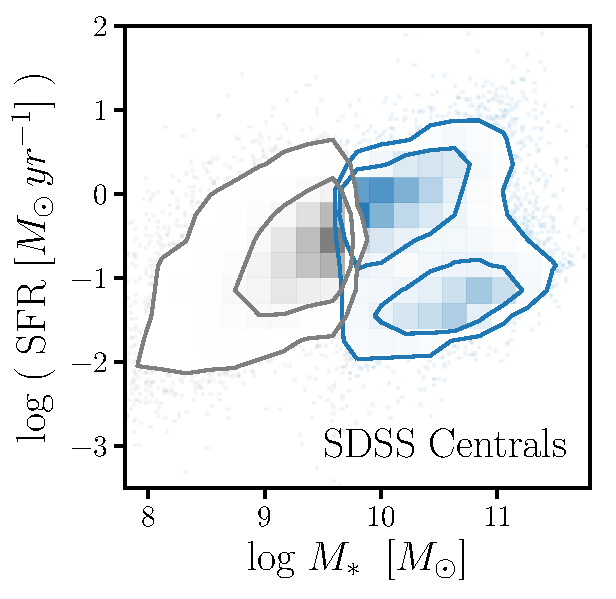
\includegraphics[width=0.45\textwidth]{Obvs_SFR_Mstar.pdf} 
\caption{\emph{Star-forming central galaxies in the SDSS 
have a well-defined relationship between their SFRs and stellar masses, 
placing them on the ``star-forming sequence''.} Our SDSS central galaxy 
sample is derived from a volume-limited sample from~\cite{tinker2011} 
at $M_* > 10^{9.7} M_\sun$ (blue) and a low luminosity sample 
from~\cite{geha2012} at $M_* < 10^{9.7} M_\sun$ (gray) described in 
Section~\ref{sec:obvs}.
}
%\todo{describe the SDSS galaxies}} 
\label{fig:sfrmstar_sdss}
\end{center}
\end{figure}
%%%%%%%%%%%%%%%%%%%%%%%%%%%%%%%%%%%%%%%%%%

%%%%%%%%%%%%%%%%%%%%%%%%%%%%%%%%%%%%%%%%%%
% Figure  
%%%%%%%%%%%%%%%%%%%%%%%%%%%%%%%%%%%%%%%%%%
%\begin{figure}
%\begin{center}
%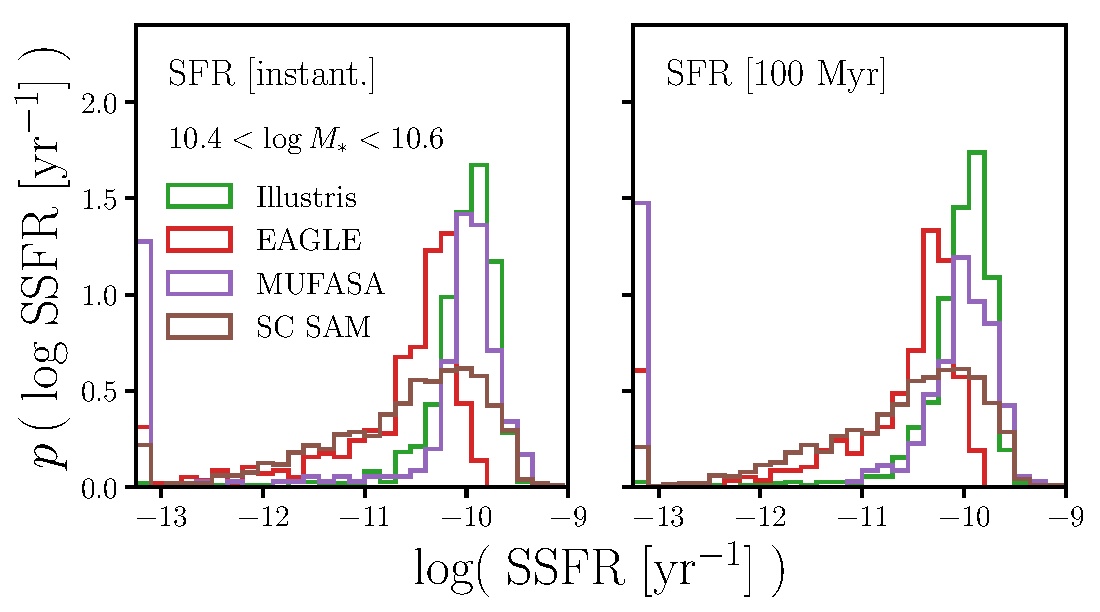
\includegraphics[width=0.475\textwidth]{figs/Catalogs_pSSFR.pdf} 
%\caption{The SSFR distributions, $p(\log\,\mathrm{SSFR})$, of the 
%central galaxies with $10.4 < \log\,M_* < 10.6$ in the Illustris (green), 
%EAGLE (red), and {\sc Mufasa} (purple) hydrodynamic simulations and the 
%SC-SAM (brown). We use instantaneous SFRs on the left and SFRs averaged 
%over $100\,\mathrm{Myr}$ on the right. Simulated galaxies with 
%$\mathrm{SFR}{=}0$ are assigned $\log\,\mathrm{SSFR}{=}-13.2$ so that they 
%can be included in the figure. Although the SFS is universal (Figure~\ref{fig:sfrmstar}), \emph{the significant 
%differences among the $p(\log\,\mathrm{SSFR})$s make the SFS 
%difficult to consistently quantify.}} \label{fig:pssfr}
%\end{center}
%\end{figure}
%%%%%%%%%%%%%%%%%%%%%%%%%%%%%%%%%%%%%%%%%%%

\section{The Galaxy Samples} \label{sec:galsims}% \label{sec:ourgals}
In this work, our main focus is to compare simulated central galaxies 
from four large-scale cosmological simulations: three hydrodynamic 
(Illustris, EAGLE, and {\sc Mufasa}) and one semi-analytic (SC-SAM). 
A consistent comparison requires consistently defined galaxy properties
across the simulations. For all of the simulated galaxies we derive 
their stellar masses using the same definition and their SFRs on two 
timescales: instantaneous and averaged over $100\,\mathrm{Myr}$. SFR 
on these timescales approximately correspond to $H{\alpha}$ 
and $UV$ based SFR measurements, which represent the formation of young 
stars with ages ${\lesssim}10\,\mathrm{Myr}$ and star formation in the 
last ${\sim}100\,\mathrm{Myr}$, respectively~\citep[e.g.][]{kennicutt2012}. 
We use instantaneous SFR, instead of SFR averaged over 
$10\,\mathrm{Myr}$, to minimize resolution effects in hydrodynamic 
simulations on such short timescales (Appendix~\ref{app:zerosfr}).

%CHH: fix up paragraph below 
In the hydrodynamic simulations, we derive the instantaneous SFRs from 
the rate of star formation in the dense and cold gas 
{\bf \color{red} 
for all the gas gravitationally bound to the host halo, and the 
$100\,\mathrm{Myr}$ averaged SFRs from the ages, or formation times, 
of all star particles  bound to the host halo (excluding stellar 
particles bound to subhalos).
} 
For the semi-analytic model, we derive the 
instantaneous SFR using the Kennicutt-Schmidt relation for molecular 
hydrogen~\citep[based on][]{bigiel2008} and the derived H$_2$ surface 
density in radial bins. We derive the SC-SAM $100\,\mathrm{Myr}$ averaged SFRs 
from the total stellar mass formed in the galaxies, which is outputted 
from the model every $10\,\mathrm{Myr}$. 

For the stellar masses of all simulated galaxies, we use the total 
stellar mass within the host halos, discounting the stellar mass in 
any subhalo within the halo. 
{\bf \color{red} 
Although stellar masses within some effective radius is better suited 
for comparison to observations (especially $M_* \gtrsim 10^{11}\ M_{\sun}$ 
galaxies), they are significantly impacted by the galaxy size predicted 
by the different sub-grid models of the simulations. Since we primarily 
focus on comparing only simulations, we use the total stellar mass within 
the halo, which is easy to consistently define. Furthermore, we test using 
the EAGLE simulation that our analysis (\emph{i.e.} the SFSs we identify) 
is {\em not} significantly impacted whether we use the total stellar masses 
within the halo or stellar masses within $70, 50,~\mathrm{or}~30\,\mathrm{kpc}$. 
We reserve a more careful comparison to observations in the next paper of
the series: Starkenburg et al. (in prep). 
}
%Furthermore, although halos are identified differently in the simulations, nearly all the stellar mass is in the center of halos. 

From the SFRs and stellar masses, we derive the specific-SFRs of the galaxies 
as $\log\,\mathrm{SSFR} = \log\,\mathrm{SFR} - \log\,M_*$. Due to the numerical 
and resolution effects a significant number of galaxies in the hydrodynamic 
simulations have $100\,\mathrm{Myr}$ averaged ``SFR$=0$'', when their SFRs 
are below the resolution limit of the simulations. We consider these galaxies 
to have ``unmeasurably low SFRs''. For the instantaneous SFRs and both SFRs for 
the SC-SAM, we analogously consider $\log\,\mathrm{SFR} < -4\ M_{\sun} \mathrm{yr}^{-1}$ 
as "unmeasureably low SFR". We discuss in Appendix~\ref{app:zerosfr} how 
we treat the effect of spatial, mass, and temporal resolution of the simulations, 
{\bf \color{red}
which can impact SFR and $M_*$, in further detail.
}
%The full halo mass range of $2 \times 10^8$ to $3\times 10^{14}\ M_{\sun}$  is set by resolution (32 particles) at the low-mass end and by volume at  the high-mass end (e.g.~including 10 halos with $M>10^{14}M_{\sun}$). 

In the rest of this section we provide a brief description of the 
Illustris, EAGLE, {\sc Mufasa}, and SC-SAM simulations and each 
of their key sub-grid and feedback prescriptions. 
\textcolor{red}{A summary of their properties can be found in Table~\ref{tab:sims}.} 
In addition, we briefly describe the
SDSS galaxy sample, which we include for reference, in Section~\ref{sec:obvs}.
Lastly, we describe how we consistently identify central galaxies among 
the simulations and observations in Section~\ref{sec:central}. 

%We compare the population of the SFR--$M_{\star}$ plane between the different large-scale cosmological simulations and the observational datasets. To ensure that we compare similar star formation rate timescales, we use averaged star formation rates over chosen recent timescales for all the simulated galaxies. For our analysis, however, we use SFRs averaged 
%over $100\,\mathrm{Myr}$ and instantaneous SFR, to be roughly consistent with respectively observed SFRs based on $H{\alpha}$ observations, corresponding to young stars with ages $\lesssim 10\,\mathrm{Myr}$, and observed SFRs based on $UV$ brightness, corresponding to stars formed in the last $\sim 100\,\mathrm{Myr}$ \citep[e.g.][]{kennicutt2012}. 

%and how  we derive the instantaneous and $100\,\mathrm{Myr}$ averaged SFRs for  each simulation.

%For the galaxies in the simulations, we compare star formation rates averaged over the last $10\,\mathrm{Myr}$, $100\,\mathrm{Myr}$, and $1\,\mathrm{Gyr}$, as well as the instantaneous SFR. 
%We note that spatial and temporal resolution effects in the simulations  can cause averaged SFRs from stellar ages to under-predict the actual  averaged SFRs in simulations. 
%(most notably the $10\,\mathrm{Myr}$--averaged SFR) can strongly under-predict the actual averaged SFR in the simulations. We therefore add conservative upper limits and uncertainties to these values and study the effect of these on our results.

%Our figures will mostly focus on comparisons of the observationally most relevant timescales (instantaneous, $10\,\mathrm{Myr}$ and $100\,\mathrm{Myr}$) but we will comment on deviations for longer or shorter timescales.

\subsection{Illustris}
The Illustris 
simulation\footnote{\url{http://www.illustris-project.org}}~(\citealt{vogelsberger2014,genel2014}; 
public data release~\citealt{nelson2015}) 
evolves a cosmological volume of $(106\ \rm{Mpc})^3$ with a uniform 
baryonic mass resolution of $1.26\times10^6M_{\sun}$ using the {\sc Arepo} 
moving-mesh code~\citep{springel2010}. 
It employs sub-grid models for star-formation~\citep{springel2003},
Bondi-like supermassive black hole (SMBH) accretion, \textcolor{red}{a phenomenological 
model for galactic winds~\citep[inspired by][]{oppenheimer2006}}, and two main modes for energy injection 
from SMBHs~\citep[see][]{vogelsberger2013}. When gas accretion onto the 
SMBH occurs at Eddington ratios $>0.05$, thermal energy is injected 
continuously in  the local environment of the SMBH. At lower accretion 
rates, the  energy injection occurs in bursts at large distances from the 
SMBH, generating hot bubbles in the intracluster medium~\citep{sijacki2007}.
%The latter mode of feedback is responsible for a steep drop in the  cosmic star-formation rate density at late times~\citep{vogelsberger2013}.
\textcolor{red}{The $z=0$ stellar mass function and the cosmic SFR 
density as a function of redshift were used to tune parameters for Illustris. 
In addition, a parameter was introduced that controls the metallicity of the 
galactic winds, which was tuned to the normalization of the $z=0$ 
stellar mass-gas metallicity relation of galaxies.}
Previous works discussing aspects of the SFS and/or quenching in Illustris 
include \citet{genel2014, vogelsberger2014, sparre2015, bluck2016, terrazas2017}.

\subsection{EAGLE}
The Virgo Consortium's Evolution and Assembly of GaLaxies and their 
Environment (EAGLE)
project\footnote{\url{http://www.eaglesim.org}}~\citep{schaye2015, crain2015} 
is a publicly available~\citep{mcalpine2016} suite 
of cosmological, hydrodynamic simulations of a standard 
$\Lambda$ cold dark matter universe. Of the simulations, we use 
L0100Ref, which has a volume of $(100\,\mathrm{comoving\,Mpc})^3$ and 
baryonic mass resolution of $1.81\times 10^6M_{\sun}$. 
It uses {\sc Anarchy} (Dalla Vecchia et al. in prep.; 
see also Appendix A of \citealt{schaye2015} and \citealt{schaller2015}), 
which is a modified version of the ${\sc Gadget}$ 3 $N$-body/SPH 
code~\citep{springel2005} 
that includes modifications to the SPH formulation, time stepping, and 
sub-grid physics. The sub-grid model for feedback from massive stars 
and AGN is based on thermal energy injection in the ISM~\citep{dallavecchia2012}.  
%Similar to semi-analytical models, 
\textcolor{red}{The sub-grid parameters for stellar feedback and BH 
accretion are calibrated to reproduce the $z=0$ stellar mass function 
and reasonable galaxy sizes. The AGN feedback efficiency is 
constrained by the central black hole-galaxy mass relation. 
The simulation resolves galaxies above $M_* > 10^{8} M_\sun$.} % and reproduce the galaxy  stellar mass function to $\lesssim 0.2~\mathrm{dex}$ over this range. 
The SFR--$M_*$ relation and quiescent fractions in EAGLE have been 
previously discussed in~\citet{furlong2015, trayford2015}
{\bf \color{red}, and the passive fraction based on mock observations in~\citet{trayford2017}}. 

\subsection{{\sc Mufasa}} \label{sec:mufasa}
{\sc Mufasa} is a hydrodynamic simulation with a box size of 
$(50\,h^{-1}\ {\rm Mpc})^3$ and particle masses of $9.6 \times 10^7\ M_{\sun}$ 
and $1.82 \times 10^7\ M_{\sun}$ for dark matter and baryons, respectively. 
It  uses {\sc Gizmo}, a code built on {\sc Gadget} that uses the Meshless 
Finite Mass hydrodynamics method~\citep{hopkins2015a} rather than SPH.  %{\sc Mufasa} is constructed  using {\sc Gizmo}, a code built  upon {\sc Gadget} where we employ the Meshless Finite Mass (MFM) hydrodynamics  method~\citep{hopkins2015a} rather than SPH.
{\sc Mufasa} includes star formation via a Kennicutt-Schmidt law based on the  molecular hydrogen 
density as computed using the sub-grid recipe in~\cite{krumholz2011}. 
It also includes two-phase kinetic outflows with scalings as predicted 
in the Feedback in Realistic Environments (FIRE) simulations~\citep{muratov2015}.
Finally, it quenches massive galaxies by keeping all non-self shielded 
gas within halos above a mass of $M_q>(1+0.48 z)\,10^{12}M_\sun$ %~\citep{mitra2015} %TKS: why was this citation removed, do you remember?
near the halos' virial temperature~\citep{gabor2015, mitra2015}. 
\textcolor{red}{{\sc Mufasa} is mainly calibrated using the 
stellar mass function. The primary variable calibrated for the 
star formation feedback was the outflow velocity relative to the circular 
velocity. There was no substantial calibration of the quenching model, 
with the key free parameter taken directly from \citep{mitra2015}}. 
The stellar mass function, gas and metal content of galaxies, and 
color-mass  diagram of {\sc Mufasa} have been previously discussed 
in~\citet{dave2016,dave2017,dave2017a}.
%These prescriptions yield predictions  that are in good agreement with a range of observations across cosmic time, including the galaxy stellar mass function evolution~\citep{dave2016}, the  gas and metal content of galaxies~\citep{dave2017b} and the color-mass diagram~\citep{dave2017}. It has some difficulties in over-quenching satellite galaxies in massive halos~\citep{rafieferantsoa2018} and likely producing  too high X-ray luminosities~(Robson et al., in prep.). 
%Modulo these caveats, {\sc Mufasa} represents a state of the art model for studying galaxy assembly, particularly for central galaxies.

\subsection{Santa Cruz Semi-Analytic Model} \label{sec:scsam}
The `Santa Cruz' SAM (SC-SAM) is a semi-analytic model run on 
merger trees from a ($147.5$ comoving Mpc)$^3$ subvolume of the 
Bolshoi--Planck dark matter only $N$-body simulations~\citep{rodriguez-puebla2016}. 
The Bolshoi--Planck simulations have particle masses of $2.21 \times 10^8 M_\sun$. 
The model includes schematic prescriptions for gas heating and 
cooling, multi-phase gas partitioning, star formation, chemical 
evolution, feedback from stars, supernovae and SMBHs, the sizes 
of galactic disks and 
bulges, and merger-induced star-bursts and structural transformations. 
The SC-SAM was first presented in~\cite{somerville1999} and 
\cite{somerville2001}, with significant updates described 
in~\cite{somerville2008}, \cite{somerville2008a}, \cite{somerville2012}, 
\cite{porter2014}, \cite{popping2014}, and \cite{somerville2015a}. In this 
work, we use the version of the SC-SAM described in~\cite{popping2014} 
and~\cite{somerville2015a}, which includes the \cite{gnedin2011} recipe 
for partitioning multi-phase gas into HI, H$_2$ and HII %(specifically we adopt the~\citealt{gnedin2011} partitioning recipe). 
based on the dark matter resolution limit,
we focus our analysis on halos with $M_h{>}10^{11} M_\sun$.
Since this roughly corresponds to $M_*{\sim}10^{8.5} M_\sun$ at 
$z\sim 0$, we impose a conservative cut of $M_* > 10^{8.8}M_\sun$. 
\textcolor{red}{The SC-SAM are calibrated based on the stellar mass--halo mass 
relation and the stellar mass function as well as the normalizations of the 
black hole mass--bulge mass relation, the stellar mass--stellar metallicity 
relation, and the cold gas mass--stellar mass relation.
}
The properties of the SC-SAM galaxy population, 
such as the quiescent fraction have been previously discussed 
in~\cite{brennan2015,somerville2015a,somerville2015,brennan2017,pandya2017}.

%We run the SC-SAM on merger  trees extracted directly from the Bolshoi--Planck dark matter-only $N$-body simulations~\citep{rodriguez-puebla2016}, using a subvolume spanning  ($100$ comoving Mpc/$h$)$^3$ for this paper. 
%Previous studies have shown that the SC-SAM reproduces well many properties  of the galaxy population both nearby and out to moderately  high-redshift~\citep[\emph{e.g.}][]{somerville2015}. In particular,  \cite{brennan2015,brennan2017,pandya2017} showed that the SC-SAM reproduces  the observed quenched fraction at $z\sim 0$ but significantly underestimates  it at $z\sim 2$. 

\subsection{Observed SDSS Galaxies} \label{sec:obvs}
%The main focus of this work is to compare galaxies from our  simulations. However, since the goal of simulations is to  reproduce observations, we include, for reference, galaxies  from the SDSS volume-limited sample and the NSA low-luminosity  galaxy sample. We provide a brief description of the two  observed galaxy samples below. 
As a reference to our comparison of the simulated galaxies,  %The main focus of this work is to compare galaxies from simulations. However, for reference, 
we include SDSS galaxies from two samples: a 
$M_*{>}10^{9.7} M_\sun$ Data Release 7~\citep[DR7;][]{abazajian2009} sample 
and a $M_* < 10^{9.7} M_\sun$ Data Release 8~\citep[DR8;][]{aihara2011} sample
(blue and gray in Figure~\ref{fig:sfrmstar_sdss}). 
At high masses, we use the volume-limited galaxy sample 
from~\cite{tinker2011} constructed from the NYU Value-Added Galaxy 
Catalog~\citep[VAGC;][]{blanton2005}. It has $M_r - 5\log(h) < -18$
and is complete for $M_* > 10^{9.7} M_\sun$. For further details, 
we refer readers to~\cite{tinker2011,wetzel2013,hahn2017b}. 
%We refer to this subsample as the ``SDSS-VAGC'' sample.

At lower stellar masses, we use the isolated dwarf galaxy sample 
of \citet{geha2012} from the NASA Sloan Atlas (NSA), a reprocessing 
of SDSS DR8. The NSA is optimized for low-luminosity objects and 
relies on the improved background subtraction technique of 
\cite{blanton2011}. The catalog extends to $z{\approx}0.055$ and 
includes re-calibrated spectroscopy~\citep{yan2011,yan2012} 
with much smaller errors\footnote{This recalibration, however, is mostly 
relevant only at small equivalent width values and hence does not 
largely affect galaxies on the SFS.}.% We refer to this  subsample as the ``SDSS-NSA'' sample.
%Dwarf galaxies are considered  isolated, and selected, when the distance from a more massive host  is $> 1.5 {\rm Mpc}$ \citep{geha2012}.

For both SDSS subsamples, the stellar masses are estimated using the 
\citet{blanton2007} $\mathtt{kcorrect}$ code, which assumes a 
\cite{chabrier2003} IMF. The SFRs are from the current release 
of~\citet{brinchmann2004}\footnote{http://www.mpa-garching.mpg.de/SDSS/DR7/}, 
where they are derived using the~\cite{bruzuala.1993} model with the 
\cite{charlot2000} dust prescription and CLOUDY \citep[version C90.04;][]{ferland1996}
emission line modeling. For galaxies classified as having an AGN or a 
composite spectrum, the SFR is measured from the $D_n4000$ index~\citep{balogh1998}. 
Additionally, for star-forming galaxies that have low S/N spectra, the SFR 
is derived from the $H{\alpha}$ luminosity~\citep{brinchmann2004}. 
We emphasize that SSFRs $\lesssim 10^{-12} \mathrm{yr}^{-1}$ should only be 
considered upper limits to the true value~\citep{salim2007}.
Given the disparate methods used for the SFR measurements, the SFRs in 
the SDSS sample do not entirely correspond to either the instantaneous 
or $100\,\mathrm{Myr}$ averaged SFRs of the simulations. Consequently, 
in this work we compare the simulations on both timescales and refrain 
from detailed comparisons to SDSS. 
%As you asked in your comment, yes the SDSS MPA-JHU star formation rates are a very mixed bag. Especially, the quenched could that can be seen at higher masses are extreme upper limits (these galaxies have no or too low S/N detected emission lines and the SFR is estimated by an interpolation of the SSFR-Dn4000 distribution for star forming galaxies). Therefore a direct comparison with SFR directly form the simulations is not really doable. The location of the main sequence maybe, but the quenched components or the width certainly not. We will do the comparison to observations in paper2, where we do mock Ha and UV and Dn4000 observations for the simulated galaxies and directly compare to the Ha, UV, and Dn4000 measurements for the SDSS sample.  We do explain this in the text (and have been iterating over how much of the SDSS data we want to discuss) but if you have suggestions about how to do this better that would be most welcome!

%Thanks for clarifying this. I would personally suggest that when you present the SDSS SFRs you just honestly say that it is a mixed bag. This also motivates looking at both instantaneous and 100 Myr, since this averages the observational uncertainty in SFR tracer type. Regarding the widths you might want to just spend 1 sentence on saying that the width is ill divined in SDSS and hence you use a 0.3 dex value from the literature (but a z=0 reference would be good). 


%%%%%%%%%%%%%%%%%%%%%%%%%%%%%%%%%%%%%%%%%%
% Table 2: fits
%%%%%%%%%%%%%%%%%%%%%%%%%%%%%%%%%%%%%%%%%%
\begin{table}
\caption{\bf \color{red} Upper table: the volume, dark matter and baryonic mass resolutions 
($m_{DM}$ and $m_b$ respectively), and softening lengths ($\epsilon$) at $z=0$ of the 
Illustris, EAGLE, MUFASA, and SC-SAM simulations described in Section~\ref{sec:galsims}. 
Bottom table: purity and completeness of central galaxies identified by our group finder, 
and cosmic star formation rate densities using either instantaneous and 100 Myr-averaged 
star formation rates.} 
\begin{center}
\begin{tabular}{p{3cm}ccccc} \toprule
%\multicolumn{3}{c}{Star-Forming Sequence power-law fit} & width \\ [3pt]
%\multicolumn{3}{c}{$\log\,\mathrm{SFR}_\mathrm{MS} = m\,(\log\,M_* - 10.5) + b$  } & \\ [3pt]
Simulation & Volume & $m_{DM}$ & $m_b$ &  $\epsilon\ (z=0)$\\ 
            & [Mpc$^3$] & [$10^6\ M_{\sun}$] & [$10^6\ M_{\sun}$] & [kpc] \\
\hline
Illustris 	& $106.5^3$	& $6.26$ & $1.26$   & $0.71\ $(baryons); $1.42\ $(DM)\\
EAGLE  		& $100^3$	& $9.7$ & $1.81$    &  $0.7$ \\
{\sc Mufasa} & $73.5^3$	& $96$ & $18.2$    &  $0.735$ \\
SC-SAM$^*$ & $147.5^3$	& $221$ & -      &   $1.475$ \\ 
\hline
\hline
Simulation & group finder & group finder & $\rho_{\rm SFR}\ $(instantaneous) & $\rho_{\rm SFR}\ $(100 Myr) & \\
            &purity & completeness & [$M_{\sun} \textrm{yr}^{-1} \textrm{Mpc}^{-3}$] & [$M_{\sun} \textrm{yr}^{-1} \textrm{Mpc}^{-3}$] & \\
            \hline
Illustris 	&  $99\%$ & $86\%$ & $10^{-1.66}$ & $10^{-1.68}$ \\
EAGLE  		&  $93\%$ & $89\%$ & $10^{-2.22}$ & $10^{-2.20}$ \\
{\sc Mufasa} &  $84\%$ & $91\%$ & $10^{-1.87}$ & $10^{-1.91}$ \\
SC-SAM$^*$ &  $97\%$ & $85\%$ & $10^{-1.94}$ & $10^{-1.94}$ \\ 
\hline
\end{tabular} \label{tab:sims}
\end{center}
{\bf \color{red}
$^*$ the SC-SAM is run on 8 subboxes from the Bolshoi-Planck dark matter only $N$-body simulations. The dark matter particle mass and softening length quoted are for the Bolshoi-Planck simulations, and the volume quoted is for the 8 combined subboxes.}
\end{table}
%%%%%%%%%%%%%%%%%%%%%%%%%%%%%%%%%%%%%%%%%%

%%%%%%%%%%%%%%%%%%%%%%%%%%%%%%%%%%%%%%%%%%%%%%%%%%%%
% Section 
%%%%%%%%%%%%%%%%%%%%%%%%%%%%%%%%%%%%%%%%%%%%%%%%%%%%
%Galaxies carry the imprint of their environment (~\citealt{hubble1936, oemler1974, dressler1980, guzzo1997},  for a recent review see~\citealp{blanton2009}). 
\subsection{Identifying Central Galaxies} \label{sec:central}
Measurements of the quiescent fraction~\citep[\emph{e.g.}][]{baldry2006,peng2010,hahn2015}
and star formation quenching timescale~\citep{wetzel2013,hahn2017b} 
suggest, whether a galaxy is a satellite or central galaxy influences 
its star formation rate. There may also be significant differences 
between the SFSs of central versus satellite galaxies~\citep{wang2018}. 
In this paper \emph{we focus solely on the central galaxies, which 
constitute the majority of massive galaxies ($M_* > 10^{9.5}M_\sun$) at $z \sim 0$}. 
%Galaxies and their detailed properties carry the  imprint of their environment (~\citealt{hubble1936, oemler1974, dressler1980, guzzo1997},  for a recent review see~\citealp{blanton2009}). The environment dependence of, for instance, the quiescent  fraction~\citep[\emph{e.g.}][]{baldry2006,peng2010,hahn2015} and the timescale of star formation quenching~\citep{wetzel2013,hahn2017},  suggest that different physical mechanisms act in different environments  to impact galaxy star formation. 

Central classification, despite its importance, is often 
heterogeneously defined in the literature. Among simulations, the 
classification depends on the definition of halo properties, 
and thus on the underlying halo finders. EAGLE and Illustris use 
$\mathtt{SUBFIND}$~\citep{springel2001}, where halos are defined as 
locally overdense, gravitationally bound (sub)structures within a 
connected region selected through a 
friend-of-friends~\citep[FOF;][]{davis1985} group finder. {\sc Mufasa} 
and SC-SAM, meanwhile, use 
$\mathtt{ROCKSTAR}$~\citep{behroozi2013}, which defines halos using a
hierarchical phase-space based FOF technique and seeks to maximize 
the consistency of the halo through time. In addition, these central 
classifications also use information of the underlying dark 
matter --- information {\em not} available in observations. Therefore, 
we identify central galaxies in all simulations consistently using %an extended version of 
the~\cite{tinker2011} group finder, designed to identify satellite/centrals 
in observations. 
%Despite the consistent definition of centrals in the simulations we use, the classification depends on the definition of halo properties in the simulation and thus differences can arise due  to differences in the underlying halo finders used. In the case of our set of simulations both EAGLE and Illustris use
%SUBFIND~\citep{springel2001}, where halos are defined as locally overdense, gravitationally bound (sub)structures within a connected region selected through a friend-of-friends~\citep[FOF]{davis1985} group finder. On the other hand {\sc Mufasa} and the Santa Cruz SAM are based on halos found using ROCKSTAR~\citep{behroozi2013}, which defines halos using a hierarchical phase-space based FOF technique and endeavors to maximize the consistency of the halo through time. Comparison projects have shown that the halo (central)/subhalo (satellite) classification generally agrees well (although the (sub)halo mass estimation can vary significantly), except when the subhalo is close to the center of the host for example during major mergers, and in late stages of minor mergers~\citep{knebe2011, behroozi2015}. 

The~\cite{tinker2011} group finder is a halo-based algorithm that uses 
the abundance matching ansatz to iteratively assign halo masses to groups. 
It assigns a tentative halo mass to each galaxy by matching the abundance 
of the objects. Then starting with the most massive galaxy, nearby lower
mass galaxies are assigned a probability of being a satellite. Once all 
the galaxies are assigned to a group, the halo masses of the central galaxies 
are updated by abundance matching with the total stellar mass in the groups. 
This entire process is repeated until convergence. In the resulting catalog, 
every group contains one central galaxy, which by definition is the 
most massive, and a group can contain zero, one, or many satellites.
For a detailed description we refer readers to~\cite{tinker2011,wetzel2012}.

Overall, we find good agreement between the central classifications of 
the group finder with respect to that of the simulations %Using purity and completeness as defined  in Eqs.~13 and~15 of~\cite{campbell2015},  %We measure central galaxy classification purities of 
with purities of 
$99\%, 93\%, 84\%$, and $97\%$ and completenesses of $86\%$, $89\%$, 
$91\%$, and $85\%$ for the Illustris, EAGLE, {\sc Mufasa} and SC-SAM 
simulations respectively 
{\bf \color{red} (Table~\ref{tab:sims}).} 
Differences in the purity and completeness for the 
simulations is likely due to the different halo finders used in the 
simulations. %For the hydrodynamic simulations, 
We find no significant stellar mass dependence in the purities. %The SC-SAM, due to  its mass resolution, has purity of $44\%$ at $M_*$ below $10^{8.5}M_\sun$  and $97\%$ above. However, as we discuss in Section~\ref{sec:scsam}, we  impose a conservative stellar mass limit of $M_* > 10^{8.8} M_\sun$. 
As expected from the high purity and completeness, when we perform our 
analysis using the centrals identified by the dark matter halos, we 
find no significant differences. %the group finder  classification does \emph{not} impact the results of this paper. 
In the next section, we proceed to fitting the star-forming sequence 
of simulated \emph{central} galaxies. % identified as centrals.

%%%%%%%%%%%%%%%%%%%%%%%%%%%%%%%%%%%%%%%%%%
% Figure 
%%%%%%%%%%%%%%%%%%%%%%%%%%%%%%%%%%%%%%%%%%
\begin{figure*}
\begin{center}
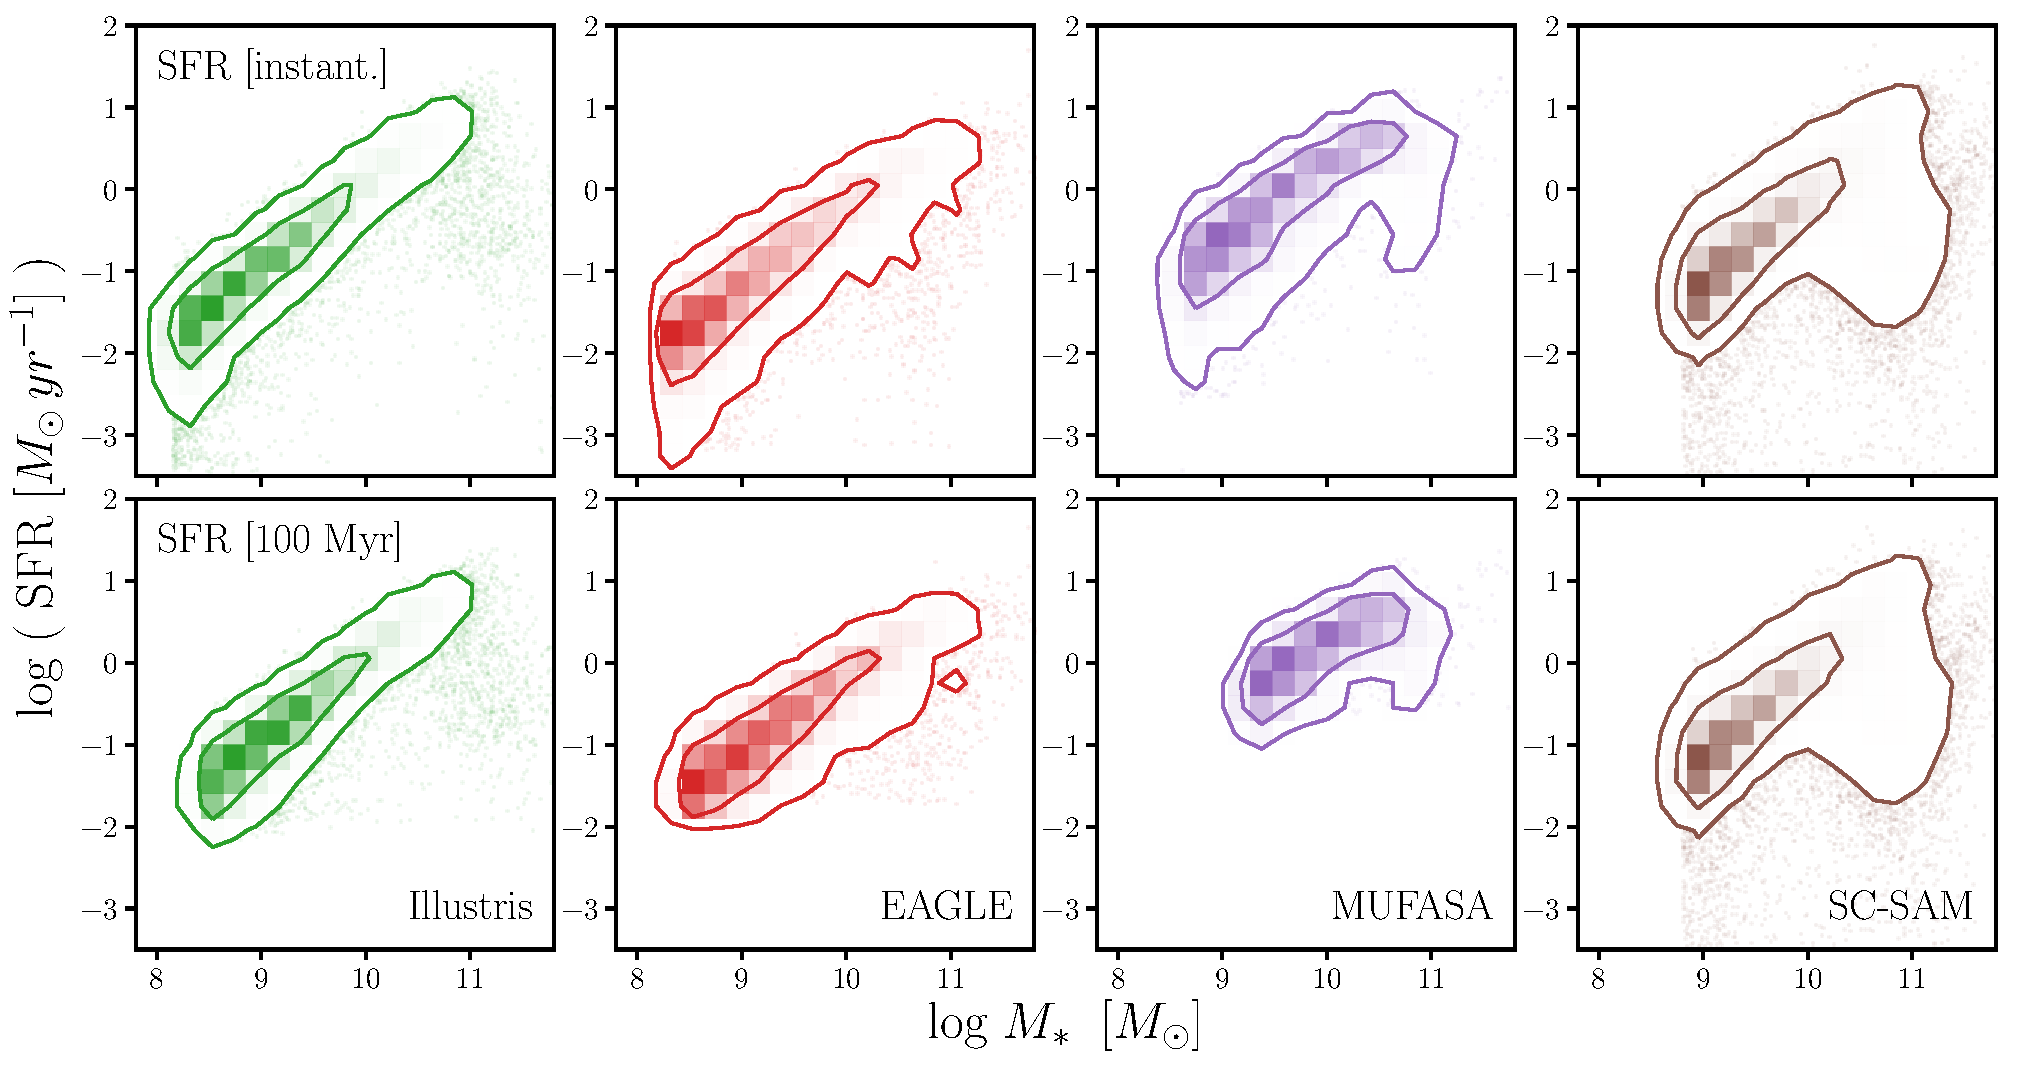
\includegraphics[width=0.95\textwidth]{Sims_SFR_Mstar.pdf} 
\caption{The SFR--$M_*$ relations of central galaxies from 
the Illustris (green), EAGLE (red), and {\sc Mufasa} (purple) hydrodynamic 
simulations and the SC-SAM (brown) at $z=0$. The top panels use instantaneous 
SFRs while the bottom panels use SFRs averaged over $100\,\mathrm{Myr}$. The 
contours in each panel mark the $68\%$ and $95\%$ confidence intervals of the 
SFR--$M_*$ distribution. We describe the simulations and how we derive consistent 
SFRs and stellar masses in Section~\ref{sec:galsims}. \emph{The SFR--$M_*$ relations 
reveal star-forming sequences in all of the simulations.}} 
\label{fig:sfrmstar}
\end{center}
\end{figure*}
%%%%%%%%%%%%%%%%%%%%%%%%%%%%%%%%%%%%%%%%%%
%%%%%%%%%%%%%%%%%%%%%%%%%%%%%%%%%%%%%%%%%%
% Figure 
%%%%%%%%%%%%%%%%%%%%%%%%%%%%%%%%%%%%%%%%%%
\begin{figure*}
\begin{center}
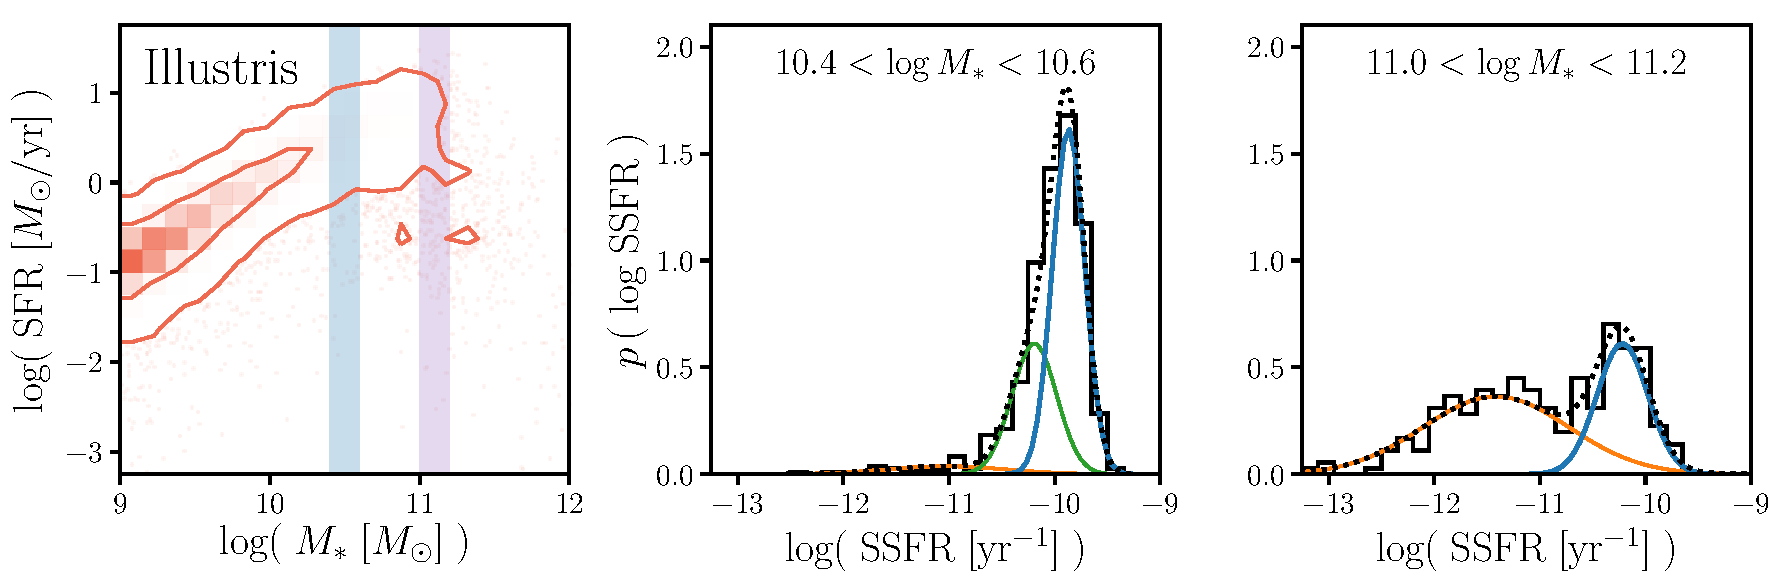
\includegraphics[width = 0.9\textwidth]{SFMSfit_demo.pdf} 
\caption{
We illustrate our 
{GMM based method for identifying the SFS of} Illustris central galaxies in two 
stellar mass bins highlighted on the SFR--$M_*$ relation of the left panel: 
$10.4 < \log\,M_* < 10.6$ and $11.0 < \log\,M_* < 11.2$. We compare the SSFR 
distributions, $p(\log\,\mathrm{SSFR})$, in the two stellar mass bins to their 
best-fit GMMs (right panels). The $p(\log\,\mathrm{SSFR})$ in the center panel is best described by a 
GMM with three components (orange, green, and blue) while the
$p(\log\,\mathrm{SSFR})$ in the right panel is best described by 
a GMM with two components (orange and blue). The SFS components of the 
best-fit GMMs are plotted in blue. \emph{Our GMM method provides
a flexible and data-driven method of identifying the SFS in a wide variety 
of SSFR distributions without hard assumptions or cuts to the sample.}
}\label{fig:fitdemo}
\end{center}
\end{figure*}
%%%%%%%%%%%%%%%%%%%%%%%%%%%%%%%%%%%%%%%%%%

\section{Identifying the Star-Forming Sequence}\label{sec:sfmsfit}
We present the SFR--$M_*$ relation of central galaxies from the 
observations and simulations of Section~\ref{sec:galsims} in 
Figures~\ref{fig:sfrmstar_sdss} and~\ref{fig:sfrmstar}. For both 
instantaneous and $100\,\mathrm{Myr}$ SFRs (top/bottom),
in both simulations and observations, and over four orders of magnitude 
in SFR and stellar mass, \emph{the SFR and $M_*$ of star-forming galaxies 
lie on a well-defined SFS.} Despite its universality, in detail, the different 
datasets give rise to different SFR--$M_*$ distributions, which makes the 
SFS difficult to consistently and meaningfully quantify. 
So far in the literature, a wide variety of fitting methods has been applied to 
data --- even in a single comparison (see Appendix~\ref{app:literature}). 
For example, in \cite{lee2015} and some of the fits in~\cite{somerville2015}
the SFS is fit using median $\log\,\mathrm{SFR}$s of galaxies after some 
color-color or SSFR cut to the sample. Other SFSs in~\cite{somerville2015} 
are fit using the median $\log\,\mathrm{SFR}$s of the entire sample. 
\cite{bluck2016} fit the SFS using median $\log\mathrm{SFR}$s of low mass 
galaxies ($M_* < 10^{10}M_\sun$) and extrapolate to higher masses. %This method, however, assumes that all $M_* < 10^{10}M_\sun$  galaxies lie on the SFS and that there is no variation in the slope  of the SFS at higher stellar masses. Alternatively, \cite{lee2015} fit the SFS using median  $\log\,\mathrm{SFR}$s of galaxies in the sample after some color-color  cut to identify SF galaxies. 
Other recent works in the literature have opted for more sophisticated 
methods such as fitting a three-component Gaussian~\citep{bisigello2018} 
or a zero-inflated negative binomial distribution~\citep{feldmann2017}. 

All of these methods require arbitrary assumptions or hard cuts to the 
sample. More importantly, for such methods, different assumptions 
or cuts produce different SFSs and inconsistent assumptions and cuts 
can result in misleading SFS comparisons (Appendix~\ref{app:literature}).
Identifying the SFS also requires flexibility in accounting 
for the different features in the galaxy property space over a wide SFR or 
$M_*$ range and in different simulations and observations.
%These methods also struggle to flexibly account for  the different features in the galaxy property space over a wide  SFR or $M_*$ range and in different simulations and observations. %for the wide variety of SSFR distributions we see  in simulations and observations. 
%Even for fixed a stellar mass bin ($10.4 < \log M_* < 10.6$),  Figure~\ref{fig:pssfr} reveals the significant differences in  the SSFR distributions of the four simulations.}
In an effort to better fit the SFS from a wide variety of SFR--$M_*$ 
distributions and to relax the assumptions and cuts imposed on the data, 
\emph{we present a flexible and data-driven method for identifying the SFS 
that makes use of Gaussian Mixture Models}.

\subsection{Using Gaussian Mixture Models} \label{sec:gmm}
Gaussian mixture models (hereafter GMM), and mixture models in general, provide 
a probabilistic way of describing the distribution of a population by 
identifying subpopulations from the data~\citep[][]{Press:1992:NRC:148286, 9780471006268}.
Besides their extensive use in machine learning and statistics, 
GMMs have also been used in a wide range of astronomical analyses~\citep[\emph{e.g.}][]{bovy2011,lee2012,taylor2015}. 
Since identifying the subpopulation of star-forming galaxies from the overall
galaxy population is equivalent to identifying the SFS, GMMs provides a 
well-motivated, data-driven, and effective method to tackle the problem. 

A GMM, more precisely, is a weighted sum of $k$ Gaussian component densities 
\begin{equation} \label{eq:gmm}
\hat{p}(x;\bm{\theta}) = \sum\limits_{i=1}^{k} \pi_i \, \mathcal{N}(x; \bm{\theta}_i),
\end{equation}
which can be used to estimate the density. The weights, $\pi_i$, mean, and 
variance $\bm{\theta}_i=\{\mu_i, \sigma_i\}$ of the components are free 
parameters. For a given data set $\{x_1, ..., x_n\}$, these 
parameters are most commonly estimated through the expectation-maximization 
algorithm~\citep[EM;][]{dempster1977,neal1998}. 

Starting with randomly assigned $\bm{\theta}_{i}^0$ to the $k$ GMM components, 
the EM algorithm iterates between two steps. First, for every data point, 
$x_i$, the algorithm computes for a probability of $x_i$ being generated by 
each GMM component. These probabilities act as assignment weights to each of
the components. Next, based on these weights, $\bm{\theta}_i^t$ of the components 
are updated to $\bm{\theta}_i^{t+1}$ to maximize the likelihood of the assigned 
data. $\pi_i$ are also updated by summing up the assignment weights and 
normalizing the sum by the total number of data points. These steps are 
repeated until $p(\{x_1, ..., x_n\} ; \bm{\theta}_t)$ converges. Instead of 
starting with randomly assigning $\bm{\theta}_{i}^0$, we initiate our EM algorithm 
using a $k$-means clustering algorithm~\citep{lloyd1982}, more specifically 
we use the $k$-$\mathtt{means}$++ algorithm~\citep{arthur2007}. 

For actually identifying the SFS, we first divide the galaxy 
sample into stellar mass bins of some width $\Delta \log M_*$. In this paper 
we use bins of $\Delta \log M_* = 0.2\ \mathrm{dex}$; however, this 
choice does not significantly impact the final SFS. For each stellar 
mass bin, if there are more than $N_\mathrm{thresh}{=}100$ galaxies in the bin, 
we fit the SSFR distribution using GMMs with $k{=}1$ to 3 components with 
parameters determined from the EM algorithm described above. 
%Our restriction to models with a maximum of 3 components is  motivated by the three main galaxy subpopulations: quiescent, star-forming,  and transitioning galaxies. More importantly, 
For the SDSS galaxy sample and all the simulations, even when we 
allow for more than 3 components, the best-fit GMMs have $k\leq3$. Hence, the 
choice of $k\leq3$ does not significantly impact the results of this work.
%Our restriction  to models with a maximum of 3 components is motivated by the three main  galaxy classifications: quiescent, star-forming, and transitioning  populations. Furthermore, for our observed galaxy samples, even when we allow for more than 3 components,  the best-fit GMMs have $k\leq3$. We confirm that restricting ourselves  to 3 components does not significantly impact the results of this work (Appendix~\ref{app:gmm}). 
Out of the three ($k\leq3$) GMMs, we select the one with the lowest Bayesian 
Information Criteria~\citep[BIC;][]{schwarz1978} as our ``best-fit'' model. 
BIC is often used in conjunction with
GMMs~\citep[\emph{e.g.}][]{leroux1992,roeder1997,fraley1998,steele2010performance} 
and also more generally for model selection in 
astronomy~\citep[\emph{e.g.}][]{liddle2007,broderick2011,vakili2016}.
{\bf \color{red}
In addition to the likelihood, BIC introduces a penalty term for the number
of parameters in the model:
\begin{equation} \label{eq:bic}
\mathrm{BIC} = -2\,\mathrm{ln}\,\mathcal{L} + N_\mathrm{par}\,\mathrm{ln}\,N_\mathrm{data}.     
\end{equation}
$N_\mathrm{par}$ is the total number of GMM parameters ($\mu_i, 
\sigma_i,$  and $\pi_i$) and $N_{\rm data}$ in our case is the 
number of galaxies in each stellar mass bin. With more components 
(and parameters), GMMs in principle can better fit the data; however, 
the BIC is lower only if the higher component GMM improves the likelihood
term more than the increase in the second term of Eq.~\ref{eq:bic}. 
In this way, using BIC for our model selection not only finds a good 
fit to the data, but it also addresses the concern of over-fitting. 
} 

Given the best-fit GMM, we next identify the SFS components in 
each $\log M_*$ bin. We start from the lowest $\log M_*$ bin, 
where we take the component with the largest weight as the SFS 
component. Then in the next higher $\log M_*$ bin we identify 
the component with the largest weight. If this component has a 
mean within $0.5\,\mathrm{dex}$ of the previous lower $\log M_*$ 
bin SFS component mean, we identify this component as the SFS. 
Otherwise, we discard it and determine whether the component with 
the next highest weight is within $0.5\,\mathrm{dex}$ of the 
previous SFS component mean. We repeat this until we either 
identify a SFS component or, if no component is within 
$0.5\,\mathrm{dex}$ of the previous SFS component mean, conclude 
that no SFS component is in the $\log M_*$ bin. We repeat this 
procedure recursively for all the $\log M_*$ bins. This scheme 
takes advantage  of the bimodality in the SSFR distributions and 
{\bf \color{red} has as its only assumption that the SFS forms a 
relatively continuous sequence. We choose $0.5\,\mathrm{dex}$ in order to relax 
any assumptions on the slope of SFS and also to avoid misclassifying 
the quiescent population as SFS at the high mass end. However, within 
the range $0.2 - 0.9\,\mathrm{dex}$, the SFSs that we identify is 
not significantly impacted.
}
In Appendix~\ref{app:gmm_pssfr}, we present a detailed comparison 
of the GMM fits to the SSFR distributions of the simulations 
and discuss the advantages of our method in further detail.


%Next, we 
%identify the component of the best-fit GMM with mean 
%$\log\,\mathrm{SSFR}{>}{-}11$ as the SFS component. 
%We mainly use this threshold to identify the high stellar mass bins 
%where no galaxies lie on the SFS. It does not impact the position of the 
%best-fit GMM components. If there are more 
%than one GMM component with mean $\log\,\mathrm{SSFR}{>}{-}11$, 
%we take the component with the larger weight as the SFS component. 

%When we compare  the $k\leq3$ GMM fits to the SSFR distribution of our simulations in three  stellar mass bins, we find good agreement between the lowest BIC best-fit  models and the SSFR distributions (Appendix~\ref{app:gmm_pssfr};  Figures~\ref{fig:pssfr_gmm_inst} and~\ref{fig:pssfr_gmm_100myr}).

In Figure~\ref{fig:fitdemo}, we illustrate our GMM based method for identifying the SFS of the Illustris central galaxies 
in two stellar mass ranges highlighted in the left panel: $10.4 < \log\,M_* < 10.6$ (center) 
and $11.0 < \log\,M_* < 11.2$ (right). For the two stellar mass bins, 
we compare the SSFR distributions of the bins to the components of the 
best-fit GMMs derived from our method. The SFS components of the best-fit 
GMMs are plotted in blue. The SSFR distribution of the center panel is best 
described by a GMM with three components while the SSFR distribution 
in the right  panel is best described by a GMM with only two components.
%The right panels illustrate the wide variation in SSFR distributions of the galaxy samples. 
These comparisons highlights the flexibility and effectiveness of our 
method in identifying the SFS for different SSFR  distributions. 
Our code for identifying the SFS makes use of the following software: 
{\em astroML}~\citep{astroML}, {\em astropy}~\citep{astropy:2013,theastropycollaboration2018}, 
{\em matplotlib}~\citep{Hunter:2007}, {\em numpy}~\citep{numpy:2011}, 
{\em scipy}~\citep{scipy:2001}, and {\em scikit-learn}~\citep{scikit-learn:2011}. 
All of the code is publicly available at \url{https://github.com/changhoonhahn/LetsTalkAboutQuench}.

%%%%%%%%%%%%%%%%%%%%%%%%%%%%%%%%%%%%%%%%%%
% Figure
%%%%%%%%%%%%%%%%%%%%%%%%%%%%%%%%%%%%%%%%%%
\begin{figure*}
\begin{center}
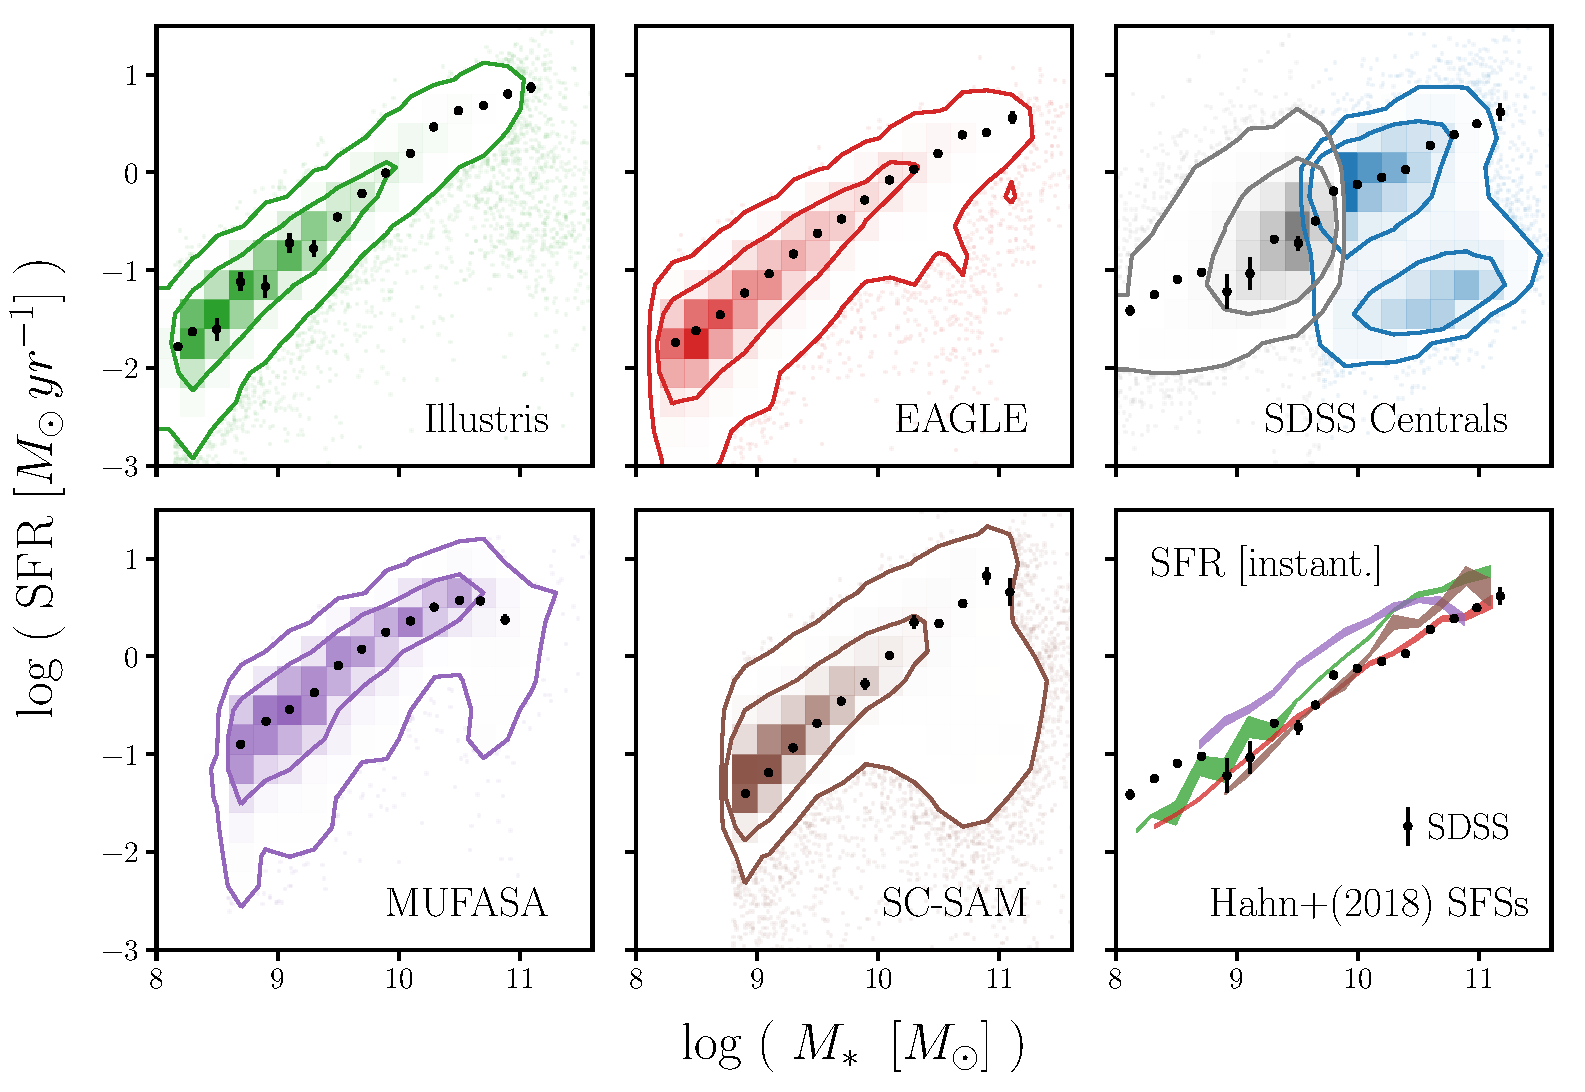
\includegraphics[width = 0.8\textwidth]{Catalogs_SFMSfit_SFRinst.pdf} 
\caption{The SFSs of the central galaxies in the Illustris, EAGLE, {\sc Mufasa}, 
    and SC-SAM simulations as identified by our GMM based method (Section~\ref{sec:sfmsfit}).
    The SFSs above are identified from the instantaneous SFR--$M_*$ relation. 
    The uncertainties of the SFSs are derived using bootstrap resampling 
    and marked by the error bars. For reference, we include the SFS of the SDSS 
    sample in the top right panel and the bottom right panel (black). 
    When we compare the \emph{SFSs of the simulations we find that they have significantly different slopes and their amplitudes vary by up to ${\sim}0.7\,\mathrm{dex}$, 
    factor of ${\sim}5$} 
    (bottom right).} \label{fig:sfmsfit_inst}
\end{center}
\end{figure*}
%%%%%%%%%%%%%%%%%%%%%%%%%%%%%%%%%%%%%%%%%%

%%%%%%%%%%%%%%%%%%%%%%%%%%%%%%%%%%%%%%%%%%
% Figure  
%%%%%%%%%%%%%%%%%%%%%%%%%%%%%%%%%%%%%%%%%%
\begin{figure*}
\begin{center}
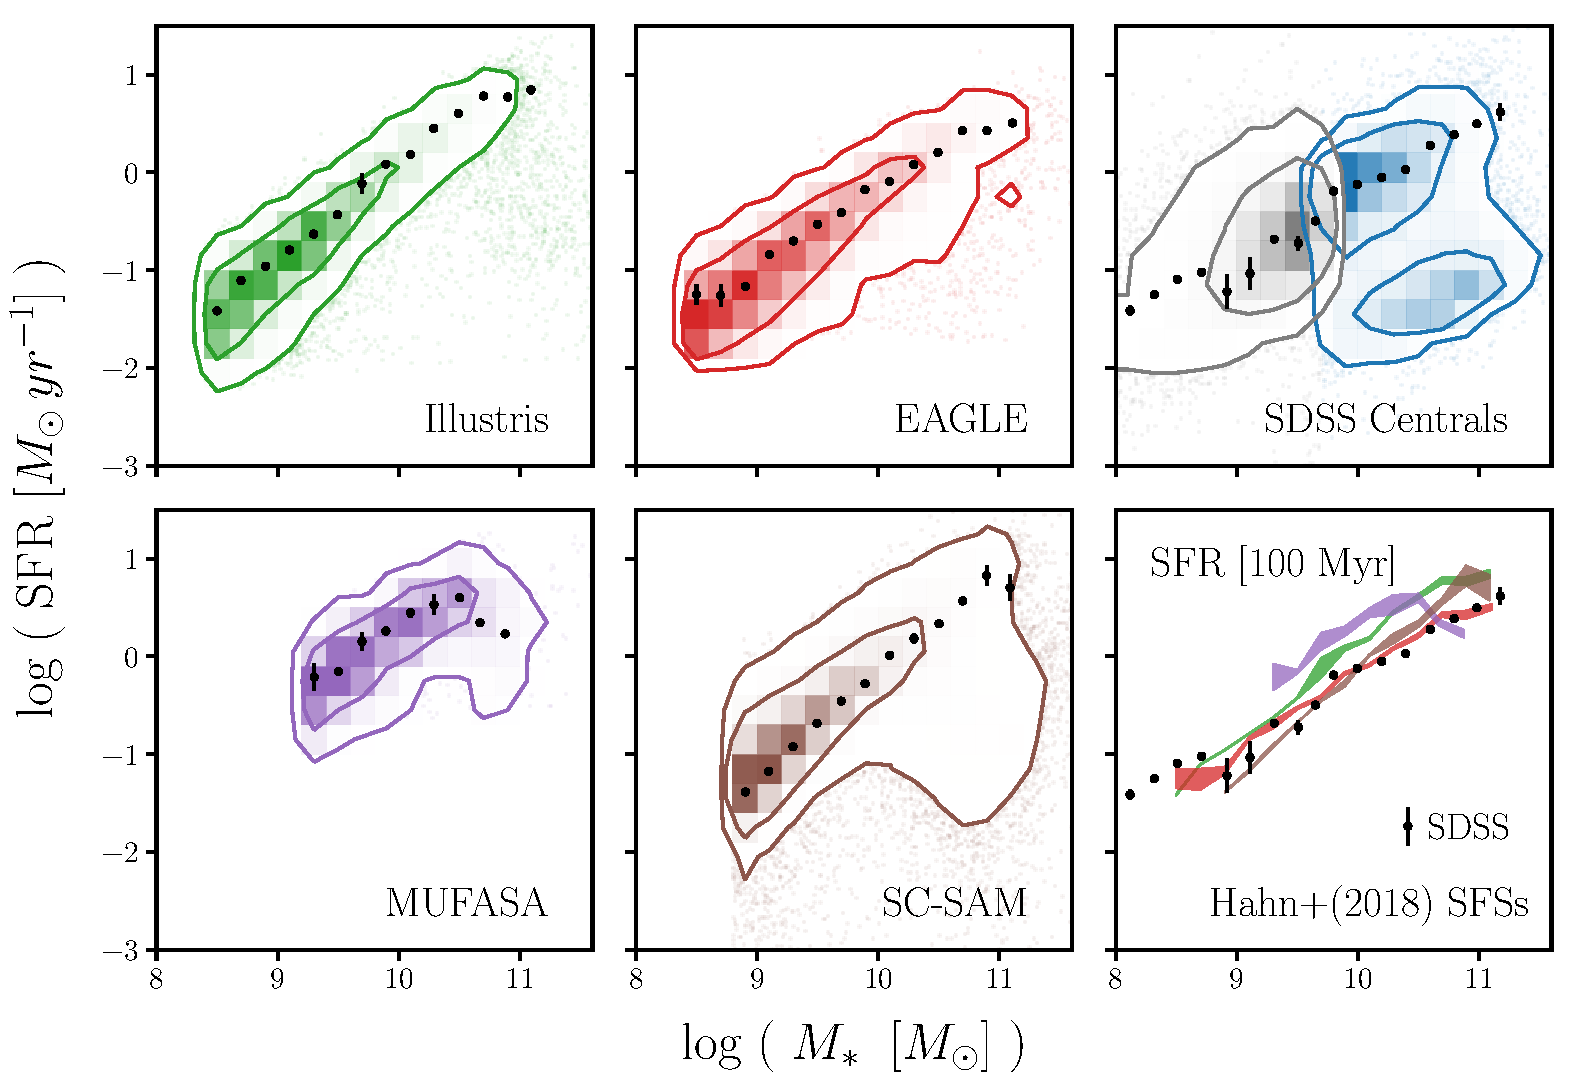
\includegraphics[width = 0.8\textwidth]{Catalogs_SFMSfit_SFR100myr.pdf} 
    \caption{Same as Figure~\ref{fig:sfmsfit_inst} but for $100\,\mathrm{Myr}$ SFR. 
    As in Figure~\ref{fig:sfmsfit_inst}, \emph{the SFSs of the simulations 
    have significantly different slopes and vary in amplitude by
    up to ${\sim}0.7\,\mathrm{dex}$, factor of ${\sim}5$}.}\label{fig:sfmsfit_100myr}
\end{center}
\end{figure*}
%%%%%%%%%%%%%%%%%%%%%%%%%%%%%%%%%%%%%%%%%%

%%%%%%%%%%%%%%%%%%%%%%%%%%%%%%%%%%%%%%%%%%
% Figure  
%%%%%%%%%%%%%%%%%%%%%%%%%%%%%%%%%%%%%%%%%%
\begin{figure}
\begin{center}
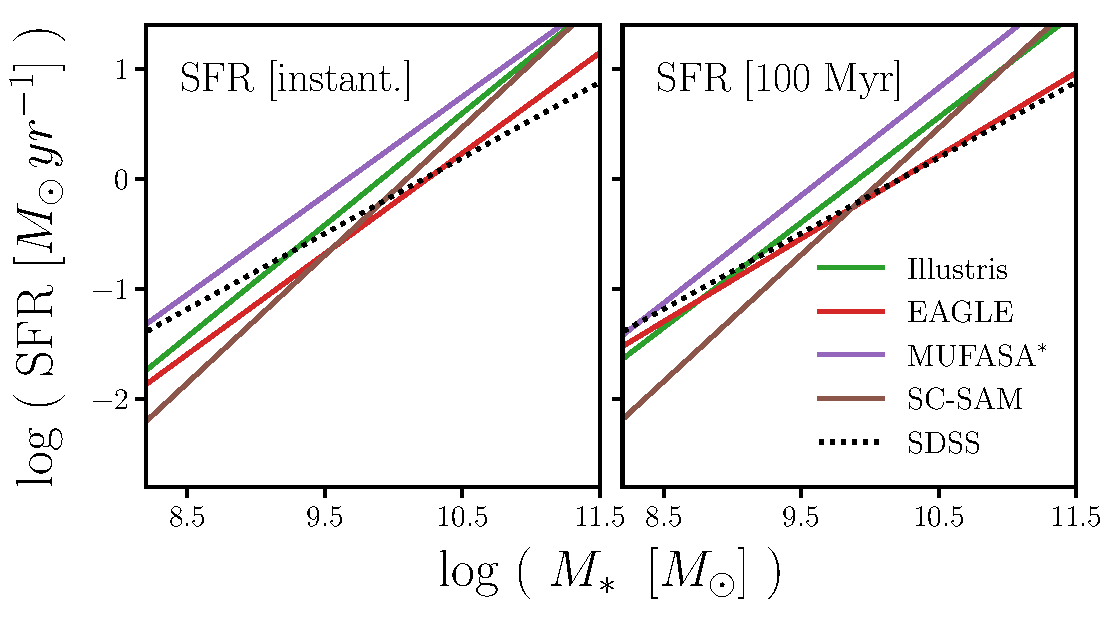
\includegraphics[width = 0.48\textwidth]{Catalogs_SFMS_powerlawfit.pdf} 
\caption{The power-law fits to the SFSs of the Illustris (green), 
    EAGLE (red), {\sc Mufasa} (purple), and SC-SAM (brown) simulations
   	highlight the significant differences in the slopes of the SFSs.
    We use instantaneous SFR and $100\,\mathrm{Myr}$ SFR in the left
    and right panels respectively. For reference, we include the 
    fit to the SDSS SFS (black dotted). We list the best-fit parameters 
    in Table~\ref{tab:sfms_powerlaw}. For a consistent comparison, we 
    fit the {\sc Mufasa} SFS below $\log\,M_* < 10.5$, due to its high stellar mass turnover.} 
    \label{fig:sfmsfit_powerlaw}
\end{center}
\end{figure}
%%%%%%%%%%%%%%%%%%%%%%%%%%%%%%%%%%%%%%%%%%

\section{Results} \label{sec:results}
\subsection{SFS of simulated galaxies} \label{sec:sfs}
Now using our GMM based method from above, % for fitting the SFS, which can be flexibly  applied a wide range of SSFR distributions, 
we can identify the SFSs of the simulated central galaxies from 
Section~\ref{sec:galsims}. We present the best-fit SFSs of the 
simulated galaxies from the Illustris, EAGLE, {\sc Mufasa}, and SC-SAM 
simulations for the instantaneous and $100\,\mathrm{Myr}$ SFR 
timescales in Figures~\ref{fig:sfmsfit_inst} and~\ref{fig:sfmsfit_100myr}, 
respectively. In each simulation, for both SFR timescales, the best-fit SFS is 
in good agreement with the underlying SFR-$M_*$ distribution as described 
by the contour and 2D histogram. However, when we compare the best-fit SFSs 
of the simulations to each another, \emph{we find that they have significantly 
different slopes and their amplitudes vary by up to 
$\,{\sim}0.7\,\mathrm{dex}$ (factor of ${\sim}5$) 
for both the instantaneous and \hunmyr~SFR timescales} 
(bottom right panels of Figures~\ref{fig:sfmsfit_inst} and~\ref{fig:sfmsfit_100myr}).
%throughout the stellar mass range of the simulations 

%The best-fit SFSs of the Illustris, EAGLE, and SC-SAM simulations
%exhibit a similar monotonic relation between SFR and $M_*$ out to 
%$M_* \gtrsim 10^{11}M_\sun$, for both SFR timescales. 
%Between the two SFR timescales, we find little difference 
%between the best-fit SFSs for each simulation. However, when we compare the 
%best-fit SFSs of the simulations altogether in more detail, we find 
%These best-fit SFSs allow us to make detailed comparison among the simulations. 
The uncertainties for the best-fit SFSs in Figures~\ref{fig:sfmsfit_inst} 
and~\ref{fig:sfmsfit_100myr} are derived from bootstrap resampling~\citep{efron1979} 
in each stellar mass bin. These uncertainties do not account for cosmic 
variance. %are  underestimates because they do not account for cosmic  variance --- \emph{i.e.} we only have one finite volume realization  of each simulation. 
Also, they correspond to the uncertainties of the means of the SFS GMM component, 
which is only one of the parameters in the GMM, and do \emph{not} account for 
the correlations other parameters of the GMM in Eq.~\ref{eq:gmm}. 
%A more  robust estimate of the uncertainties would involve estimating the marginalized  posterior distribution of the SFS GMM component mean using a method like MCMC. Since this still does not account for cosmic variance, we use bootstrap uncertainties. 
Our SFS uncertainties are estimated 
similarly to the cluster red sequence fits in~\cite{hao2009}, which use an 
``error-corrected'' GMM that involves bootstrap resampling. \cite{hao2009}, 
however, use their method to estimate the mean of their GMM component, 
rather than to estimate its uncertainty.

%Given the best-fit SFSs, we can parameterize the SFS to some 
Using the SFSs we identified, we can now parameterize it to 
some functional form as often done in the literature --- \emph{e.g.} 
power-law~\citep{speagle2014} or broken power-law~\citep{lee2015}. With 
little evidence of a turnover in the SFS in {\em most} of simulations, 
we fit a power-law of the form 
\begin{equation} \label{eq:powerlaw}
\log\,\mathrm{SFR}_\mathrm{MS} = m\,(\log\,M_* - 10.5) + b
\end{equation}
to the SFSs in Figure~\ref{fig:sfmsfit_powerlaw}. Unlike the SFS of 
other simulations, the SFSs for {\sc Mufasa} have a significant 
turnover at $M_*{\sim}10^{10.5}M_\sun$. This turnover is \emph{not} 
caused by  misidentification of the SFS or some systematic effect in the 
GMM fitting. Instead, the turnover is due to the halo mass 
dependent quenching prescription in {\sc Mufasa} (Section~\ref{sec:mufasa}), 
which causes a sharper cut-off in the SFS, unlike the other more 
self-consistent AGN feedback models. We focus on the power-law portion 
of the {\sc Mufasa} SFS and fit Eq.~\ref{eq:powerlaw} below the turnover 
($M_*{<}10^{10.5} M_\sun$). 

The best-fit (least squares) power-law parameters (Table~\ref{tab:sfms_powerlaw} 
and Figure~\ref{fig:sfmsfit_powerlaw}) highlight the significant %The power-law parameterizations accentuate the stellar mass dependence of  the SFSs and can reveal the mass dependence in the SFS discrepancies. 
differences in the slope of the SFSs. Among our simulations, $m$ ranges 
from sub-linear in {\sc Mufasa} ($0.75$) to super-linear in SC-SAM ($1.17$).  
Various sub-grid models (\emph{e.g.} ISM, star  formation, stellar and 
AGN feedback; see also \citealt{torrey2014}) can influence the slope 
and normalization of SFSs in the 
simulations. To resolve the underlying cause behind the difference in SFSs, 
would require a detailed comparison of the different sub-grid parameters 
and prescriptions. While such a comparison is beyond the scope of this 
paper, the discrepancies we find in the SFSs provide constraints on 
galaxy formation models. Furthermore,
although a detailed comparison with observations is complicated by the 
differences in how SFR is defined in simulations versus observations, 
we include in Figure~\ref{fig:sfmsfit_powerlaw} the power-law fit to the 
SFS of the SDSS central galaxies (black dotted). Compared to the SFSs of the 
simulations, SFS in SDSS has a significantly a lower slope: $m=0.69$. As a 
result, the SFSs of the simulations are scattered around the SDSS SFS 
below $M_*{\sim}10^{10} M_\sun$, but have higher amplitudes than the SDSS SFS 
above $M_*{\sim}10^{10} M_\sun$. This is also apparent in the bottom right 
panel comparisons of Figures~\ref{fig:sfmsfit_inst} and~\ref{fig:sfmsfit_100myr}. 

%The power-law SFS fits highlight the discrepancy in the slopes of the SFSs. However, they reveal no significant  stellar mass dependence in the SFS amplitude discrepancies.  
%Although the power-law SFS fits highlight the stellar mass dependence of the SFSs, they reveal   no consistent stellar mass dependence in the discrepancies of the SFSs. 
%For both SFR timescales, the discrepancies among the SFSs range from $0.5 - 1.\,\mathrm{dex}$  throughout the stellar mass range (Figure~\ref{fig:sfmsfit_powerlaw}). 

%The discrepancies between the instantaneous SFR SFSs of Illustris, EAGLE, and SC-SAM range from $1.\,\mathrm{dex}$ at low $M_*$ to $0.5\,\mathrm{dex}$ at high $M_*$ . Meanwhile, 
%for $100\,\mathrm{Myr}$ SFR, we find slightly greater discrepancies among Illustris, EAGLE, and SC-SAM throughout the stellar mass range.
The differences we find among the SFSs of the simulations, also appear in their 
cosmic star formation densities. Cosmic star formation density roughly corresponds to the total 
star formation in the SFS weighted by the stellar mass function (SMF). For Illustris,
EAGLE, {\sc Mufasa}, and SC-SAM, respectively, we find total cosmic star formation 
densities (including satellites) of 
$10^{-1.66}, 10^{-2.22}, 10^{-1.87}$, and $10^{-1.94}\,M_\sun \mathrm{yr}^{-1} \mathrm{Mpc}^{-3}$ 
using instantaneous SFRs and similarly 
$10^{-1.68}$, $10^{-2.20}$, $10^{-1.91}$, and $10^{-1.94}\,M_\sun \mathrm{yr}^{-1} \mathrm{Mpc}^{-3}$
using $100\,\mathrm{Myr}$ SFRs 
{\bf \color{red} (Table~\ref{tab:sims})}. 
The rank order of the densities is different than that of the
SFSs due to differences in the SMFs. Although these values are 
roughly within the uncertainties of observations~\citep{madau2014}, 
the difference in the star formation density between Illustris and 
EAGLE, for example, is greater than $0.5\,\mathrm{dex}$--- more 
than factor of 3.
{\bf \color{red}
With the differences among the simulations in both their cosmic star 
formation densities and SMFs, it is difficult to attribute the difference 
of the SFSs to either stellar mass or SFR alone. Differences in both properties, 
and therefore the full star formation history as modeled by different sub-grid 
prescriptions in the four simulations, likely contribute to the discrepancies 
in the cosmic SFR densities, the SMFs, and the SFSs. 
%More importantly, the difference we find in SFSs highlight the fact that the simulations predict significantly different SFR-$M_*$ relations for the star-forming galaxy subpopulation, which provides a strong constraint on galaxy formation models. 
}
%The difference in the rank ordering of the SFS amplitudes  versus the star formation density come from the discrepancies in the SMFs of  the simulations. For example, {\sc Mufasa} has the highest SFS for most of the  $M_*$ range in Figures~\ref{fig:sfmsfit_inst} and~\ref{fig:sfmsfit_100myr}).  Its SMF, however, has an overall lower amplitude than Illustris and SC-SAM. Hence  it has a SF density similar to SC-SAM and lower than Illustris.

%In fact, these star formation densities
%are more or less consistent with observations~\citep{madau2014}. 
%{\color{red}
%The cosmic star formation densities roughly correspond to the total 
%star formation in the SFS weighted by the stellar mass function (SMF).
%The SMFs of the simulations are less discrepant than the SFSs; as
%a result, the cosmic SF densities have smaller discrepancies. }

%CHH: clarify the SDSS sigma is measurement uncertainties
In addition to its position, $\mu_\mathrm{SFS}$, the SFS GMM component 
is also described by $\sigma_\mathrm{SFS}$ --- the width of the SFS. 
Using $\sigma_\mathrm{SFS}$ derived from the GMM fitting, 
we can compare the width of the SFS among the simulations 
(Figure~\ref{fig:sfms_width}). The uncertainties for the widths are 
calculated through bootstrap resampling in the same way as the SFS 
uncertainties. Overall, we find little stellar mass  dependence in 
$\sigma_\mathrm{SFS}$ for the simulations. For Illustris, EAGLE, 
{\sc Mufasa}, and SC-SAM we respectively find 
$\sigma_\mathrm{SFS}{\sim}0.20, 0.26, 0.25$, and $0.24\,\mathrm{dex}$ 
for instantaneous SFR and
$\sigma_\mathrm{SFS}{\sim}0.18, 0.20, 0.25$, and $0.23\,\mathrm{dex}$
for $100\,\mathrm{Myr}$ SFR (Table~\ref{tab:sfms_powerlaw}). 
Although we do not explicitly include the width of the SDSS SFS GMM 
component due to inconsistencies in the SFRs~(Section~\ref{sec:obvs}), 
these $\sigma_\mathrm{SFS}$ are narrower than the ${\sim}0.3\,\mathrm{dex}$ 
width measured in  observations~\citep[\emph{e.g.}][]{daddi2007, noeske2007, salim2007, magdis2012, whitaker2012, speagle2014}. 
{\bf \color{red} 
Observational errors, however, will bring the simulated values to 
closer agreement. For instance, the SFRs of our SDSS galaxies from 
the NYU-VAGC have measurement errors of 
$\sigma_{\log\,\mathrm{SFR}} \approx 0.031\,\mathrm{dex}$, approximated 
from repeated SFR measurements of the same galaxies. Furthermore, the 
hydrodynamic simulations lack burstiness caused by 
clustered star formation, and thus feedback due to resolution effects. 
\citet{sparre2017a} found that burstiness can increase $\sigma_{\log\,\mathrm{SFS}}$ 
by $0.10-0.17\,\mathrm{dex}$. Additionally, \citet{genel2018} recently 
showed that chaotic effects can contribute to the overall scatter in the SFS. 
However, since we derive $\sigma_\mathrm{SFS}$ from a large galaxy population 
this butterfly effect does not impact the measurement reliability of statistical 
properties of the ensemble of galaxies because the sensitivity of individual 
galaxy SFRs averages out. However, the different degree of the 
butterfly effect on different simulations may contribute the difference 
in $\sigma_\mathrm{SFS}$  among the simulations.
} % However, they note that this butterfly effect does not impact  statistical properties of the ensemble of galaxies because the sensitivity  of individual galaxy SFRs averages out. Since we derive $\sigma_\mathrm{SFS}$  from a large galaxy population, our measurements are likely unaffected.  However, the different degree of the butterfly effect on different  simulations may contribute the difference in $\sigma_\mathrm{SFS}$  among the simulations.
This unresolved variability will also bring the scatter closer to 
the observed width. %This difference, however, does not account for the uncertainties in the observed SFR measurements, which would reduce the discrepancy.
We therefore conclude that \emph{the width of the SFS from the simulations 
are in reasonable agreement with the observed SFS width.}



%%%%%%%%%%%%%%%%%%%%%%%%%%%%%%%%%%%%%%%%%%
% Table 2: fits
%%%%%%%%%%%%%%%%%%%%%%%%%%%%%%%%%%%%%%%%%%
\begin{table}
\caption{Power-law fit to the SFS of the simulated central galaxies from the
Illustris, EAGLE, {\sc Mufasa}, and SC-SAM simulations.} 
\begin{center}
\begin{tabular}{p{3cm}ccc} \toprule
\multicolumn{3}{c}{Star-Forming Sequence power-law fit} & width \\ [3pt]
\multicolumn{3}{c}{$\log\,\mathrm{SFR}_\mathrm{MS} = m\,(\log\,M_* - 10.5) + b$  } & \\ [3pt]
Simulation & $m$ & $b$ & $\sigma_\mathrm{SFS}$ [dex] \\ 
\hline
\multicolumn{4}{c}{Instantaneous SFR} \\
Illustris 			& 1.01 $\pm$ 0.004 & 0.59 $\pm$ 0.006 & 0.20 \\ 
EAGLE 				& 0.91 $\pm$ 0.006 & 0.23 $\pm$ 0.008 & 0.26 \\ 
{\sc Mufasa} 		& 0.75 $\pm$ 0.014 & 0.58 $\pm$ 0.011 & 0.25 \\ 
{\sc Mufasa}$^*$ 	& 0.89 $\pm$ 0.020 & 0.74 $\pm$ 0.020 &  \\ 
SC-SAM 				& 1.17 $\pm$ 0.008 & 0.48 $\pm$ 0.009 & 0.24 \\ 
\hline \hline
\multicolumn{4}{c}{$100\,\mathrm{Myr}$ SFR} \\
Illustris 			& 0.95 $\pm$ 0.006 & 0.55 $\pm$ 0.008 & 0.18 \\
EAGLE  				& 0.75 $\pm$ 0.010 & 0.21 $\pm$ 0.009 & 0.20 \\
{\sc Mufasa}		& 0.38 $\pm$ 0.023 & 0.36 $\pm$ 0.016 & 0.25 \\
{\sc Mufasa}$^*$ 	& 0.97 $\pm$ 0.050 & 0.83 $\pm$ 0.039 & \\ 
SC-SAM 				& 1.16 $\pm$ 0.008 & 0.47 $\pm$ 0.009 & 0.23\\ 
\hline
\hline \hspace{10pt}
SDSS 				& 0.69 $\pm$ 0.008 & 0.18 $\pm$ 0.007 \\ 
\hline
\end{tabular} \label{tab:sfms_powerlaw}
\end{center}
$^*$ power-law fit to the {\sc Mufasa} SFS below its turnover ($\log\,M_* {<}\,10.5$)
\end{table}
%%%%%%%%%%%%%%%%%%%%%%%%%%%%%%%%%%%%%%%%%%

One factor that impacts the SFS we identify is the strict lower limit of the 
$\log\mathrm{SFR}$s caused by the resolution effects in the simulations. 
This is particularly evident in the $100\,\mathrm{Myr}$ SFR--$M_*$ 
relations of the hydrodynamic simulations of Figure~\ref{fig:sfrmstar} --- especially 
{\sc Mufasa}. As we describe in Section~\ref{sec:galsims}, the $100\,\mathrm{Myr}$ 
SFRs are  calculated using the ages of all star particles in a galaxy. For a galaxy to 
have star formation (\emph{i.e.} SFR $> 0$), it must \emph{at least} 
form one star particle over the last $100\,\mathrm{Myr}$. A single star particle 
forming over $100\,\mathrm{Myr}$ amounts to a SFR of 
${\sim}0.02\ M_{\sun} \mathrm{yr}^{-1}$ for Illustris and EAGLE and
${\sim}0.2\ M_{\sun} \mathrm{yr}^{-1}$ for {\sc Mufasa}. This resolution limit, ultimately 
impacts the SFS at $M_*{<}10^{8.4}$, $10^{8.4}$, and 
$10^{9.2}M_\sun$ for Illustris, EAGLE, and {\sc Mufasa} respectively (see Appendix~\ref{app:zerosfr}). 

Using our method for identifying the SFS, we are able to 
conduct a consistent data-driven comparison of the SFSs of simulated 
central galaxies from the Illustris, EAGLE, {\sc Mufasa}, and SC-SAM. From 
this comparison, we find that the amplitudes of the SFSs differ from one 
another by up to ${\sim}0.7\,\mathrm{dex}$, factor of ${\sim}5$, 
with significantly different slopes. Furthermore, despite these differences, the SFSs of 
the simulations have similar widths, consistent with observations. 
%%%%%%%%%%%%%%%%%%%%%%%%%%%%%%%%%%%%%%%%%%
% Figure  
%%%%%%%%%%%%%%%%%%%%%%%%%%%%%%%%%%%%%%%%%%
\begin{figure}
\begin{center}
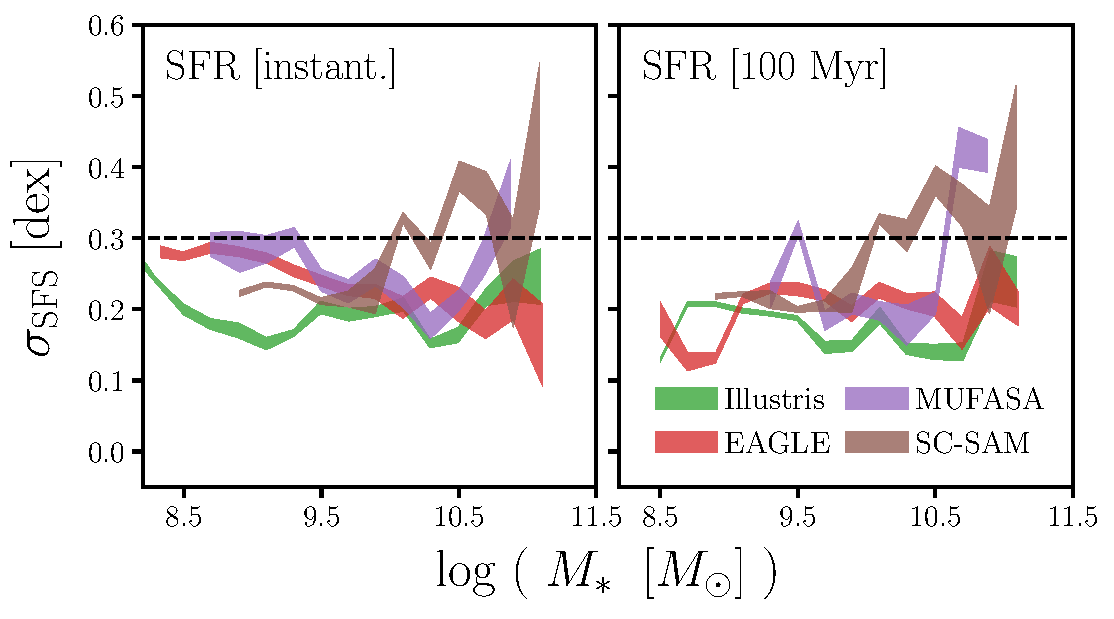
\includegraphics[width=0.48\textwidth]{Catalogs_SFMS_width.pdf}
\caption{The width of the SFS, $\sigma_\mathrm{SFS}$, for the simulated 
    central galaxies from Illustris, EAGLE, {\sc Mufasa}, and SC-SAM 
    (green, red, purple, and brown respectively). The uncertainties are 
    estimated using bootstrap resampling in the same way as the SFS uncertainties. 
    The SFS widths in the simulations have little stellar mass 
    dependence and, adding observational measurement errors in SFR, 
    they are roughly consistent with ${\sim}0.3\,\mathrm{dex}$ 
    from observations (black dashed).} \label{fig:sfms_width}
\end{center}
\end{figure}
%%%%%%%%%%%%%%%%%%%%%%%%%%%%%%%%%%%%%%%%%%

%%%%%%%%%%%%%%%%%%%%%%%%%%%%%%%%%%%%%%%%%%
% Figure  
%%%%%%%%%%%%%%%%%%%%%%%%%%%%%%%%%%%%%%%%%%
\begin{figure*}
\begin{center}
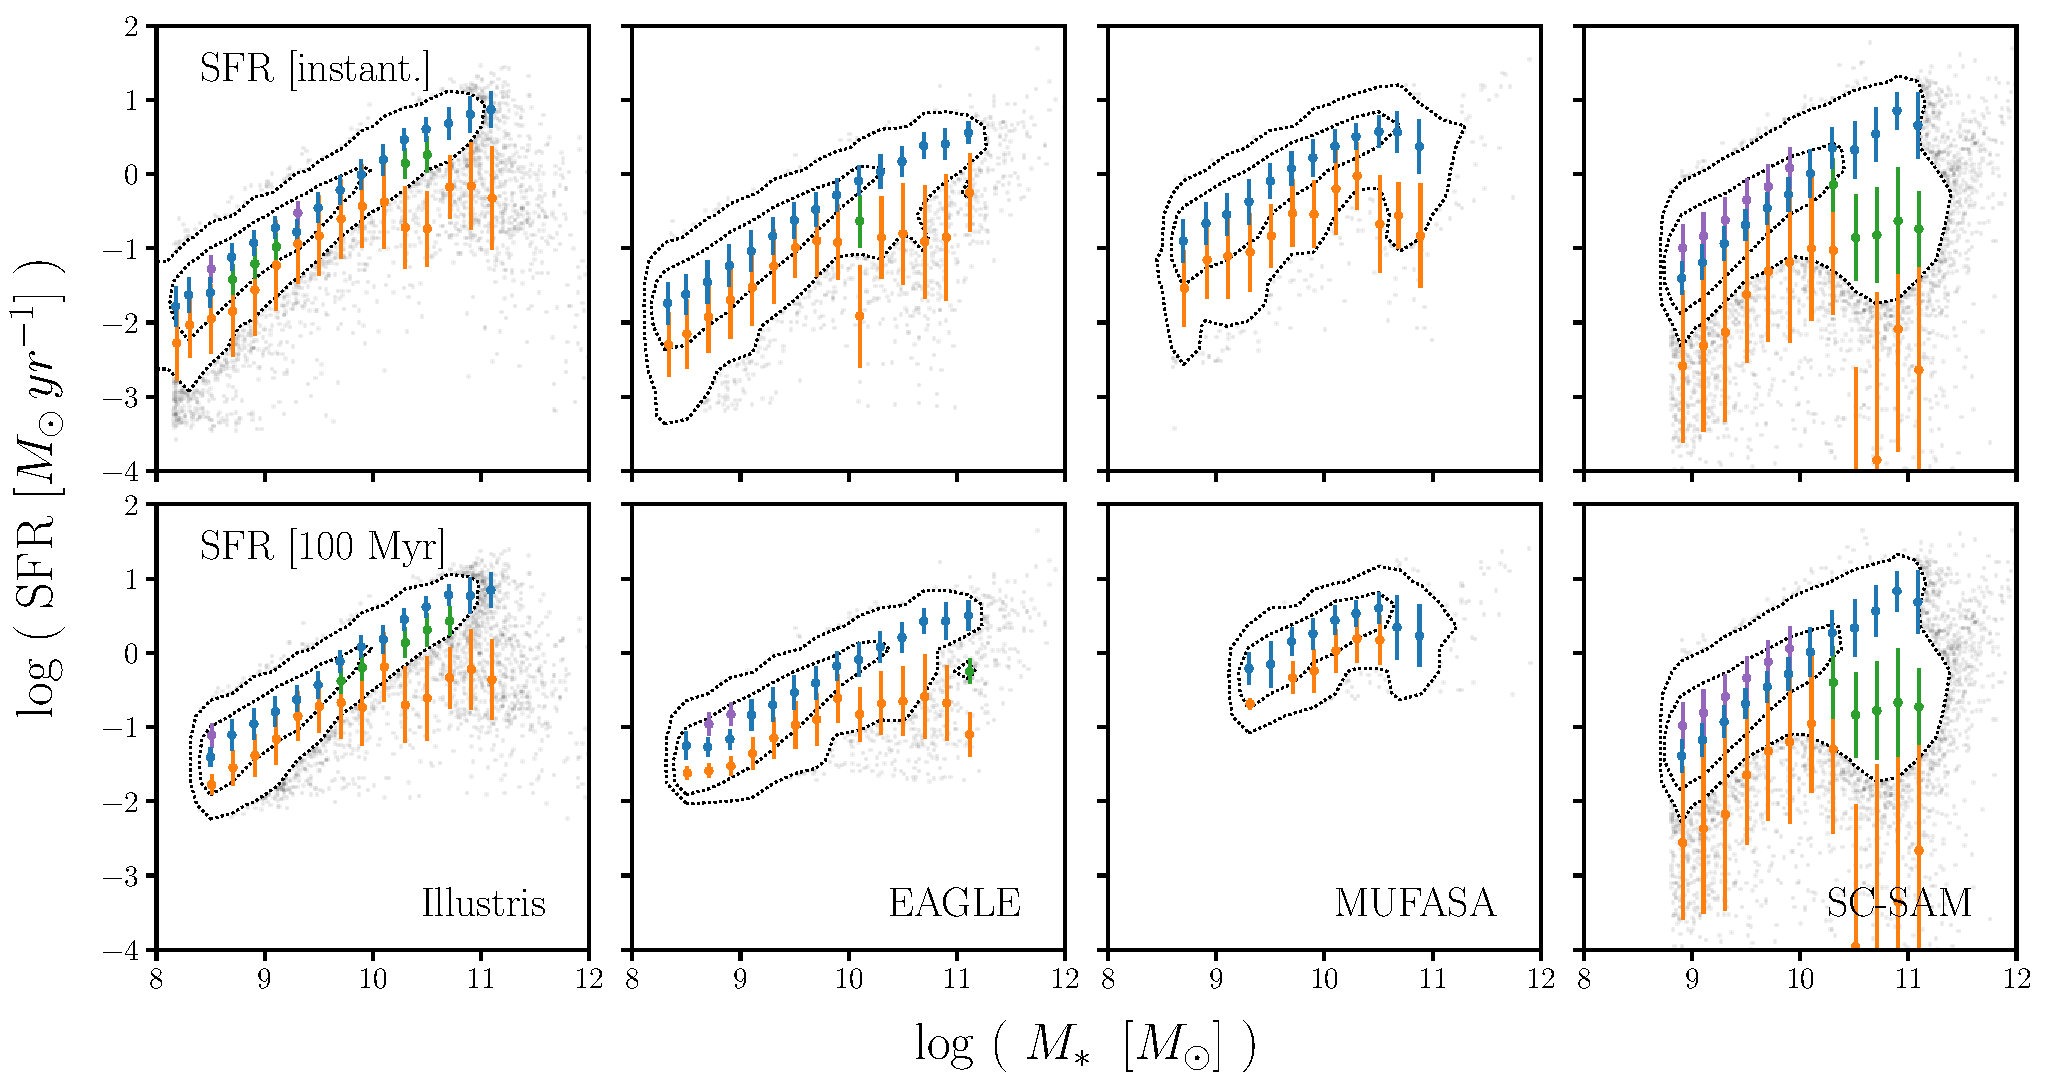
\includegraphics[width=0.95\textwidth]{Catalogs_GMMcomps.pdf} 
\caption{Components of the best-fit GMM for the SFR-$M_*$ relations of central 
    galaxies in the Illustris, EAGLE, {\sc Mufasa}, and 
    SC-SAM simulations (left to right). The top and bottom panels use instantaneous 
    SFRs and $100\,\mathrm{Myr}$ SFRs respectively. In each $\log M_*$ bin, we mark 
    the SFS component in blue, the low SF component in orange, the intermediate SF 
    component in green, and the component above the SFS in purple. These components 
    \emph{loosely} correspond to the star-forming, quiescent, transitioning, and 
    star-burst subpopulations. The hydrodynamic simulations have similar 
    subpopulations dominated by the SFS and low SF components. Meanwhile in the 
    SC-SAM, the GMM components reveal broad low SF components that extends out to 
    $\mathrm{SFR} < 10^{-4}M_\sun \mathrm{yr}^{-1}$, prominent intermediate components at 
    $M_* \gtrsim 10^{10}M_\sun$, and components above the SFS at $M_* \lesssim 10^{10}M_\sun$.} \label{fig:sfmsfit_comps}
\end{center}
\end{figure*}
%%%%%%%%%%%%%%%%%%%%%%%%%%%%%%%%%%%%%%%%%%

%%%%%%%%%%%%%%%%%%%%%%%%%%%%%%%%%%%%%%%%%%
% Figure 
%%%%%%%%%%%%%%%%%%%%%%%%%%%%%%%%%%%%%%%%%%
\begin{figure*}
\begin{center}
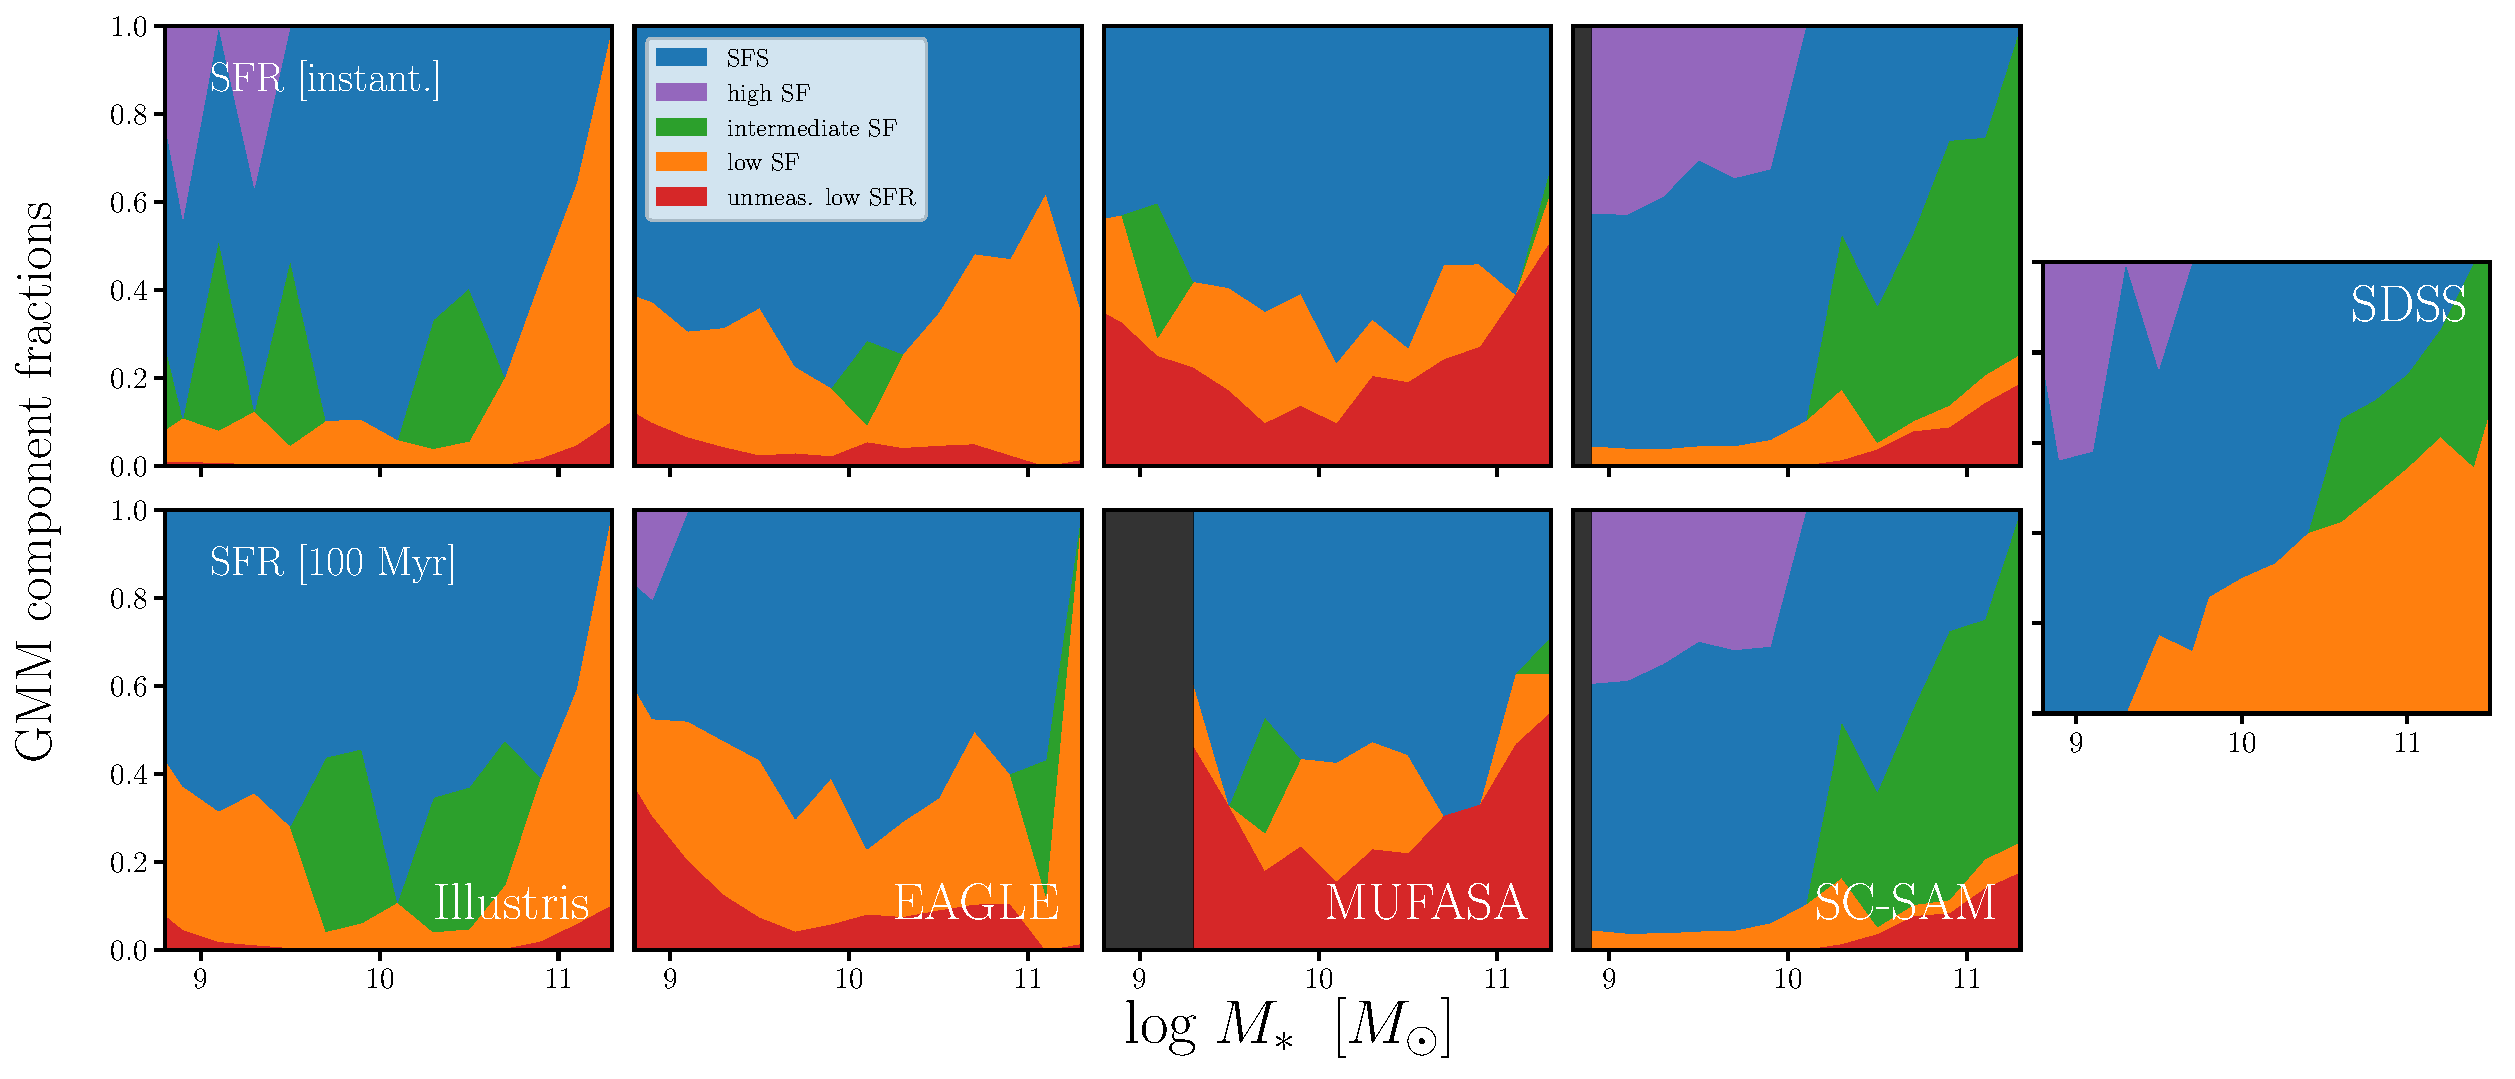
\includegraphics[width=\textwidth]{GMMcomp_composition.pdf} 
\caption{Fractional contributions, $\pi_i$, of the best-fit GMM components of 
    the central galaxies in Illustris, EAGLE, {\sc Mufasa}, and SC-SAM (left 
    to right). We highlight the SFS component in blue, the low SF component 
    in orange, galaxies with unmeasurably low SFR in red, the intermediate SF 
    components in green, and the high SF components in purple. We shade the 
    regions below the stellar mass limit set by resolution effects in black 
    (Appendix~\ref{app:zerosfr}). For reference, we include $\pi_i$ of the 
    observed SDSS centrals in the rightmost panel. Unlike SDSS or the SC-SAM, 
    we do not find significant high SF components at low $M_*$ in the hydrodynamic
    simulations. Furthermore, treating the components below the SFS as quiescent,
    we find little $M_*$ dependence in the quiescent fraction at $M_* < 10^{11}M_\sun$
    unlike observations. In fact, in all of the simulations, we find a significant 
    fraction of quiescent central galaxies at $M_* \lesssim 10^9 M_\sun$ contrary to observations.} \label{fig:kandinsky}
\end{center}
\end{figure*}
%%%%%%%%%%%%%%%%%%%%%%%%%%%%%%%%%%%%%%%%%%

%%%%%%%%%%%%%%%%%%%%%%%%%%%%%%%%%%%%%%%%%%
% Figure 
%%%%%%%%%%%%%%%%%%%%%%%%%%%%%%%%%%%%%%%%%%
%\begin{figure*}
%\begin{center}
%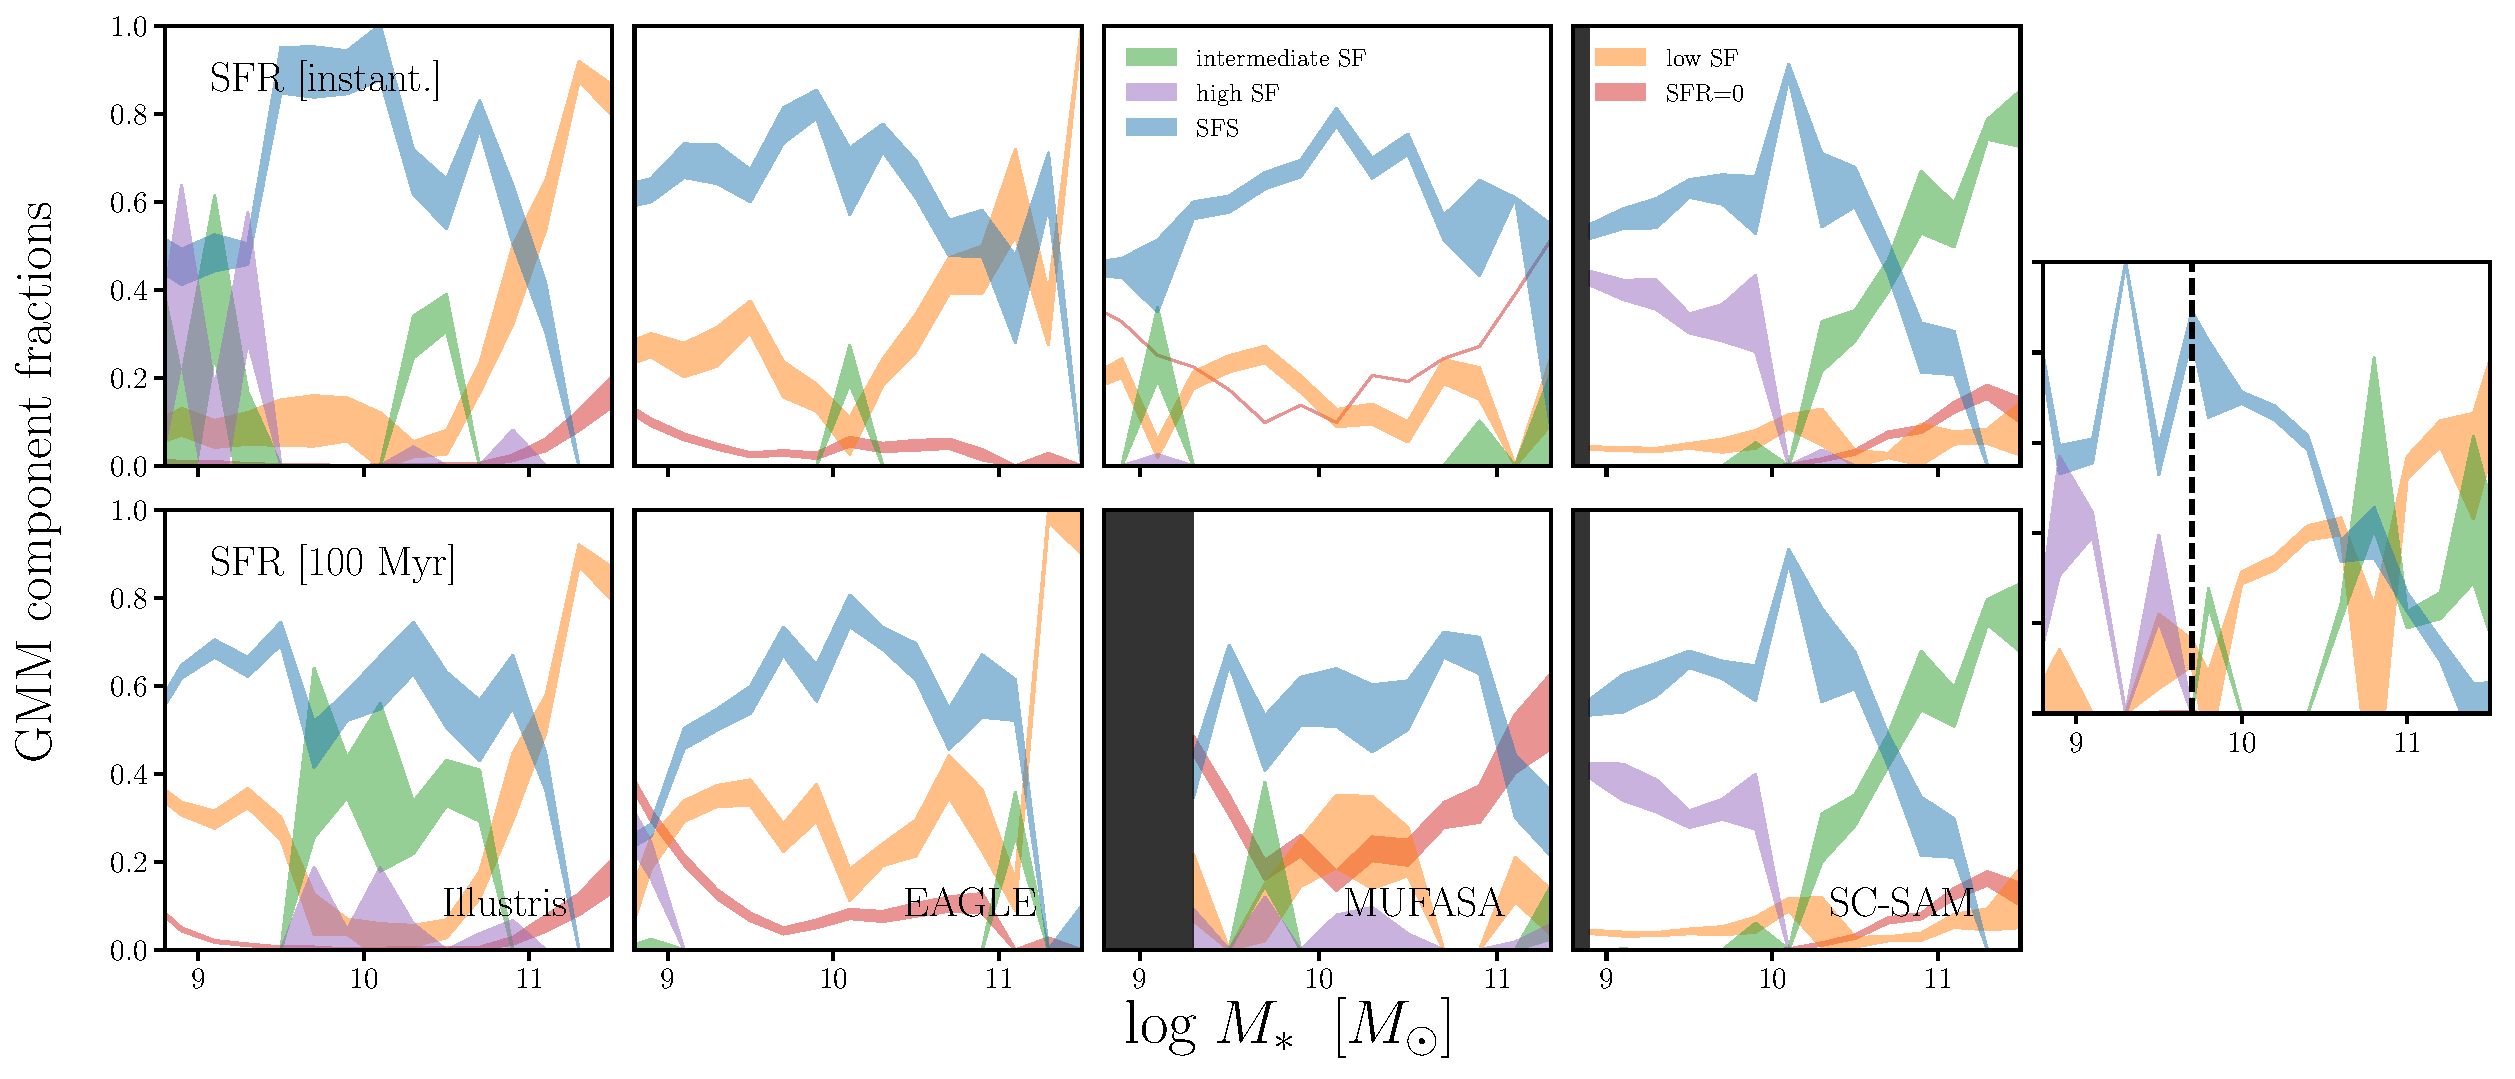
\includegraphics[width=\textwidth]{figs/GMMcomp_comp_uncertainty.pdf} 
%\caption{Uncertainties in the fractional contributions, $\pi_i$, of the 
%best-fit GMM components from our SFS fitting from Figure~\ref{fig:kandinsky}.
%The uncertainties are estimated through bootstrap resampling. 
%We plot the SFS component in blue, the quiescent component in orange, 
%galaxies with SFR$=0$ in red, the transitioning components in green, and 
%the star-burst components in purple. For reference, we include $\pi_i$ of 
%the observed centrals from SDSS and NSA in the rightmost panel.
%} \label{fig:fcomp_uncertainty}
%\end{center}
%\end{figure*}
%%%%%%%%%%%%%%%%%%%%%%%%%%%%%%%%%%%%%%%%%%
\subsection{Beyond the SFS of Simulated Galaxies} \label{sec:beyondsfms}
So far we have focused solely on the SFSs of the simulated galaxies --- \emph{i.e.} 
$\bm{\theta}_\mathrm{SFS} = \{\mu_\mathrm{SFS}, \sigma_\mathrm{SFS} \}$ 
in Eq.~\ref{eq:gmm}. Our GMM method, however, also determines 
$\bm{\theta}_i$ of components other than the SFS. These GMM components 
provide extra features to compare the simulated galaxy samples and also 
offer interesting insights into the different subpopulations in the simulated 
galaxy samples. When we examine $\bm{\theta}_i$ of all components from 
our fitting for the simulated galaxies, we find they loosely correspond 
to galaxy subpopulations typically referred to as quiescent, transitioning, 
and star-burst (Figure~\ref{fig:sfmsfit_comps}). 
{\bf \color{red}
From the data alone, we cannot determine whether the components we 
identify are actually the ``true'' sub-populations.
Therefore, to avoid over-interpreting 
}
this correspondence, we refer to the GMM component with the lowest SFR as 
``low SF'' component, the component with SFR in between the SFS and the 
low SF component as the ``intermediate SF'' component, and finally the 
component with higher SFR than the SFS component as the ``high SF'' component. 
At a given stellar mass bin, our GMM fits are restricted to $k\leq3$; hence, 
the four different components come from different stellar mass bins. 
In Figure~\ref{fig:sfmsfit_comps}, we mark the SFS, low SF, intermediate SF, 
and high SF in blue, orange, green, and purple respectively.

Examining the GMM components of the hydrodynamic simulations in 
Figure~\ref{fig:sfmsfit_comps}, we find that a few $\log M_*$ bins have 
intermediate SF components in Illustris at $10^9 M_\sun < M_* < 10^{11}M_\sun$.
Also a few of the lowest $\log M_*$ bins in Illustris and EAGLE have high SF
components for the $100\,\mathrm{Myr}$ SFRs. Besides these few 
bins, however, the central galaxies from the hydrodynamic simulations are
dominated by the SFS and low SF components. Furthermore, 
throughout the stellar mass ranges of the simulations, the low SF 
components in each of these simulations have relatively constant widths and 
lie ${\sim}1\,\mathrm{dex}$ below the SFS components.

Unlike the hydrodynamic simulations, however, the low SF components in the 
SC-SAM span out to $\log\mathrm{SFR}{=}{-}4\ M_\sun \mathrm{yr}^{-1}$. 
Furthermore, the intermediate 
and high SF components are much more prominent in the SC-SAM centrals. 
At low stellar masses ($M_* \lesssim 10^{10}M_\sun$) every $\log M_*$ 
bin has a high SF component. The $\log\,\mathrm{SSFR}$ distributions in these 
bins have extended tails on the higher SFR side of the SFS. Our GMM 
method, thus, fits high SF components in these $\log M_*$ bins (bottom left 
and center panels of Figures~\ref{fig:pssfr_gmm_inst} and~\ref{fig:pssfr_gmm_100myr}). 
These high SF components and the extended range of low SF components are likely 
caused by the re-accretion prescription of the SAM (Section 2.7 of~\citealt{somerville2008a}).
A fraction of gas ejected from halos (\emph{e.g.} from supernovae) is kept in 
a reservoir, which re-collapses into the halos at a later time and becomes available 
again for cooling. The rate of this re-accretion depends on the mass of ejected gas, 
the dynamical time of the halo, and a free parameter degenerate with supernovae 
feedback parameters. This prescription results in bursty 
star formation in the SC-SAM galaxies and causes the extended low SF components and 
the high SF components. %galaxies to have broad range of  SFRs.

%The rate of this re-accretion/infall depends on $\chi_\mathrm{re-infall}$, a free parameter, the mass of ejected gas, and the dynamical time of the halo.
% This gas is assumed to accrete on to the halo on a time-scale that is proportional to the halo dynamical time
% The fraction of gas that is ejected from the disc but retained in the halo, versus ejected from the disc and halo, is a function of the halo circular velocity (see S08 for details), such that low-mass haloes lose a larger fraction of their gas. The gas that is ejected from the halo is kept in a larger reservoir, along with the gas that has been prevented from falling in due to the photoionizing background. This gas is assumed to accrete on to the halo on a time-scale that is proportional to the halo dynamical time (see S08 for details)

At high stellar masses ($M_* \gtrsim 10^{10}M_\sun$) every $\log M_*$ bin in the 
SC-SAM has an intermediate component. While the $\log\,\mathrm{SSFR}$ 
distributions in the bottom right panels of Figures~\ref{fig:pssfr_gmm_inst} 
and~\ref{fig:pssfr_gmm_100myr} and the BIC values illustrate the benefit of the 
GMM with an intermediate SF component, these are accentuated by the broader 
distribution of the low SF population. Despite these differences between the 
hydrodynamic simulations and the SC-SAM, all of the simulations have a low SF 
component throughout their stellar mass 
range, even at $M_* < 10^9M_\sun$. We discuss these low $M_*$ low SF galaxies 
in further detail later in this section.

Another set of parameters we infer from our GMM fitting is the weight of the 
GMM components: $\pi_i$ in Eq.~\ref{eq:gmm}. These weights correspond to 
the fractional contribution of the different subpopulations. For example, the 
weight of the low SF component loosely corresponds to the quiescent 
fraction~\citep[\emph{e.g.}][]{borch2006, bundy2006, iovino2010, geha2012, hahn2015}. 
In Figure~\ref{fig:kandinsky}, we present the fractional contribution of the 
components from our best-fit GMM, as a function of stellar mass: SFS (blue), 
low SF (orange),  intermediate SF (green), and high SF (purple). We also include
the fractional contribution of galaxies with unmesurably low SFRs (red; 
see Section~\ref{sec:galsims}). The $\pi_i$ have 
uncertainties, estimated from bootstrap resampling, on the order of ${\sim}0.1$.

%We present the uncertainties of $\pi_i$s,  estimated through bootstrap resampling, in Figure~\ref{fig:fcomp_uncertainty}. 
For every simulation, a significant fraction of galaxies have unmeasurably 
low SFRs. In hydrodynamic simulations, a galaxy with unmeasureably low SFR 
can have an SFR below the resolution limit, or have a ``true'' $\mathrm{SFR}{=}0$ 
on the measured timescales (Appendix~\ref{app:zerosfr}). For the SC-SAM, we 
consider the SFR unmeasurably low when $\log \mathrm{SFR}< {-}4\ M_\sun \mathrm{yr}^{-1}$. 
Therefore, in both hydrodynamic simulations and the SAM, galaxies with 
unmeasurably low SFR can be considered quiescent. 
Moreover, we confirm that SFR resolution does not significantly 
impact the fraction contributions of Figures~\ref{fig:kandinsky} 
(see Appendix~\ref{app:zerosfr} and Figure~\ref{fig:mlim_fcomp}).%and~\ref{fig:fcomp_uncertainty} 

The fractional contributions of the GMM components in Figures~\ref{fig:kandinsky} % and~\ref{fig:fcomp_uncertainty} 
reveal significant disagreements between the simulated galaxies and 
trends established from observations--- especially the hydrodynamic 
simulations. 
For instance, in the hydrodynamic simulations we do not find significant 
high SF components at low $M_*$, unlike in SDSS or SC-SAM. The few $M_*$ 
bins with fractional contributions from high SF components have large 
bootstrap uncertainties (${\sim}0.2$). %\todo{high SF disagreement between SDSS and hydro}. SC-SAM does well.
Furthermore, if we treat the components below the SFS as quiescent 
(green, orange and red in Figure~\ref{fig:kandinsky}),
\emph{we find little stellar mass dependence in the quiescent fraction of the 
hydrodynamic simulations, unlike the quiescent fraction measurements 
of isolated SDSS galaxies}~\citep{baldry2006,peng2010,hahn2015}. 
Meanwhile, at $M_*{>}10^9M_\sun$ the SC-SAM is roughly consistent with 
SDSS (rightmost panel) and in agreement with previous 
SC-SAM quiescent fraction comparisons to observations~\citep{brennan2015,brennan2017,pandya2017}.

Furthermore, for some of the hydrodynamic simulations in 
Figure~\ref{fig:kandinsky} (Illustris, EAGLE, and {\sc Mufasa} with 
$100\,\mathrm{Myr}$ SFRs and EAGLE, and {\sc Mufasa} instantaneous SFRs)
we find surprisingly high quiescent fractions (${\sim}0.4$) at low masses in stark 
contrast with observations~\citep{baldry2006,peng2010,hahn2015}. In fact, 
\emph{all the simulations, even the SC-SAM, have non-negligible (${\gtrsim}10\%$) 
quiescent fraction at $M_*{<}10^9 M_\sun$ contrary to the $M_*$ lower bound of 
${\sim}10^9M_\sun$ for isolated/central quiescent galaxies 
we observe in SDSS and established in the literature~\citep[\emph{e.g.}][]{geha2012}.}

One possible explanation for the significant fraction of low SFR galaxies
at low $M_*$ in the hydrodynamic simulations is misclassification of 
``splashback'' (or ``blacksplash'' or ``ejected'') galaxies as centrals. 
Splashback galaxies are satellite galaxies that have orbited outside 
the virial radii of its host halo after having passed through 
it~\citep[\emph{e.g.}][]{mamon2004,gill2005,wang2009a,wetzel2014}.
The SC-SAM is {\em not} subject to this misclassification because subhalos 
are not tracked after first infall, so by construction the 
model does not have splashbacks. To test whether splashbacks 
impact our results for the hydrodynamic simulations, we adjust our central
galaxy selection criteria in Section~\ref{sec:central} to exclude 
any centrals within three virial radii of a more massive halo.
When we use this stricter central classification and measure the
SFS and other GMM components, we find \emph{no} significant change to 
the SFS fits or the fractional contributions of the GMM components. 
We also find no significant changes to our results when we restrict 
the selection to galaxies with no ``luminous'' neighbors within 
$1.5\,\mathrm{Mpc}/h$ --- analogous to the~\cite{geha2012} criteria.
We therefore conclude that the significant fraction of low SFR and 
low $M_*$ galaxies is not caused by misclassification of centrals.

%@CHH: rephrase the high res eagle stuff because at the moment it's a bit misleading.
Another possible explanation for the abundance of low SFR galaxies
at low $M_*$, is that the hydrodynamic simulations have insufficient
resolution for galaxies with $M_*{<}10^9M_\sun$. Low $M_*$ galaxies 
in reality, may have star-forming clumps with masses lower than the 
baryonic particle mass. Such star formation will not be captured by 
the simulations~\citep{sparre2017a}. We test whether our results are 
impacted by the resolution limit using a higher resolution box ($8\times$ 
higher baryon mass resolution) for EAGLE. 
{\bf \color{red} Although the fractional contributions of the low SFR GMM
component is significantly lower at $M_* \sim 10^{10}M_\sun$, this can also be affected by the low number of galaxies in this mass range in the small high-resolution box. We still find an abundance of low SFR galaxies
at $M_*<10^9M_\sun$ for the higher resolution EAGLE simulation, but as the fraction increases toward lower masses we cannot rule out resolution as the cause of the low-mass low-SFR component. 
}
%emphasize that this simply may be due to insufficient resolution of galaxies with M* < 10^9 Msun. For example, in the real Universe, such galaxies have star-forming clumps with masses less than the baryonic particle mass, and such star formation will consequently be missed in the hydro sims. This is even true of much higher-resolution zooms, and we discuss this in some detail in the Sparre et al. (2017) FIRE paper.

Taking a step back, we emphasize that this discrepancy between the 
simulations and observations must be taken with a grain of salt and
our comparison is not an apples-to-apples comparison. For instance,
in \cite{geha2012} low SF/quiescent galaxies are classified based on 
a $H\alpha$ emission and $D_n 4000$ criteria --- different than in 
the simulations. Even the central (isolation in~\citealt{geha2012}) 
criteria, in detail, is different than the analogous criteria 
above. More broadly, the comparisons we present in this paper are 
among simulations and therefore are based on ``theoretical'' predictions 
of galaxy properties. Many factors make it difficult 
to robustly extend this comparison to observations. 

For example, SFR and $M_*$, the galaxy properties considered in this paper, 
in simulations can be directly measured either using star or gas particles in 
the simulations. In observations, even the SFR alone is estimated from SFR indicators 
such as $H\alpha$ flux, $D_n 4000$, or UV brightness and dust absorption measurements. 
While they serve as estimates of the SFRs, as \cite{speagle2014} find, even 
for the same SDSS galaxies, different SFR indicators can produce large 
discrepancies in the slope and amplitude of the SFS. 
{\bf \color{red} For $M_*$, since we include all stellar particles to compute 
the stellar masses in the simulations, this may overestimate $M_*$, in 
particular for high mass galaxies. However, as we mention in Section~\ref{sec:galsims}, 
for the EAGLE sample, the SFS we identify does not change when we use stellar 
mass and SFR in the entire subhalo or within apertures of $70, 50,$ or $30\,\mathrm{kpc}$.
}
Furthermore, a 
consistent comparison to observations requires a thorough understanding of 
the selection effects that come with the observed galaxy sample. These 
effects are difficult to propagate into SFR and $M_*$ space of simulations. 

%classifications in \cite{geha2012} are defined differently than in the simulations. 
%\cite{geha2012} classifies as a galaxy as quenched if it
%does not have an $H\alpha$ emission and based on a $D_n 4000$ criteria. 
%Furthermore, the isolation criteria of \cite{geha2012} is more 
%stringent than the group finder at these mass scales. 

Therefore, while we note some of the differences in 
Figures~\ref{fig:sfmsfit_inst},~\ref{fig:sfmsfit_100myr},~\ref{fig:sfmsfit_powerlaw}, 
and~\ref{fig:kandinsky}, between the simulations and observations,  
%can see from Figures~\ref{fig:sfmsfit_inst},  \ref{fig:sfmsfit_100myr}, and \ref{fig:kandinsky} that there are significant discrepancies between the simulations and observations in the slope and  amplitude of the SFS and also the fractional contribution of the best-fit  GMM components, 
we reserve a more detailed comparison to the next paper in our 
series: Starkenburg et al. in prep. In this next paper, instead of
comparing the ``theoretical'' galaxy properties, we forward model galaxy 
spectra and photometry of simulated galaxies using their star formation 
histories, make observationally motivated measurements of SFR and $M_*$ on
the synthetic spectra and photometry, and conduct a quantitative, 
apples-to-apples, comparison of the simulations to observations.

In this section, we demonstrate that our method for identifying the SFS
provides additional features besides the SFSs, to compare different galaxy 
samples. These extra components offer insights into the 
distinct galaxy subpopulations of the simulations. Based on the non-SFS 
components/populations, we find that the hydrodynamic simulations are 
similarly dominated by the SFS and low SF components, while the SC-SAM 
predicts substantial fractions of high and intermediate SF components. 
Moreover, we find that all of the simulations have a significant
fraction of low SFR central galaxies at $M_*\,{\lesssim}\,10^9M_\sun$, 
contrary to observations. Furthermore, the hydrodynamic simulations, at 
even $M_*\,{\lesssim}\,10^{11}M_\sun$, do not reproduce the quiescent 
fractions from the literature or their stellar mass dependence. 

\section{Summary and Conclusions} \label{sec:summary}
The Star-Forming Sequence provides a key feature in galaxy property 
space to consistently compare %is a well-defined feature in the galaxy  property space that provides a key feature to consistently compare
galaxy populations in simulations and observations.
%of both simulations and observations. It provides  a key feature to consistently compare the galaxy populations of  simulations and observations. 
%provides a key feature in galaxy property  space to consistently compare the galaxy populations in simulations and observations. 
Such comparisons are crucial for validating our theories of
galaxy formation and evolution. However, they face two main challenges: 
the lack of a consistent data-driven method for identifying the SFS and 
the discrepancies in methodology for deriving galaxy properties such as 
SFR and $M_*$. In this paper, we address the former by presenting 
a flexible data-driven method for identifying the SFS. 

Our method takes advantage of Gaussian mixture models to fit the SFR
distributions in stellar mass bins and Bayesian Information Criteria 
for model selection. This data-driven approach allows us to robustly 
fit the SFR-$M_*$ relation of galaxy populations and identify the SFS, 
while relaxing many of the assumptions and hard cuts that go into 
other methods. Furthermore, it allows us to identify the SFS over a wide 
range of star formation and stellar masses down to 
$M_*{\sim}10^{8}M_\sun$. Finally, our method also allows us to identify 
subpopulations of galaxies, beyond the SFS, that correspond to the 
quiescent, transitioning, and star-burst galaxy populations. 

Next we apply our method to the central galaxies of the Illustris, EAGLE, 
and {\sc Mufasa} hydrodynamic simulations and the Santa 
Cruz semi-analytic model. The central galaxies are identified in the  
simulations using the \cite{tinker2011} group 
finder and have \emph{consistently} derived $M_*$ and SFRs on instantaneous 
and $100\,\mathrm{Myr}$ timescales. For reference, we also apply our 
method to central galaxies from SDSS observations. Comparing the resulting 
SFSs and other components from the simulations and observations, we find the following:

\begin{itemize}
\item The identified SFSs of Illustris, EAGLE, {\sc Mufasa}, and SC-SAM 
vary by up to ${\sim}0.7\,\mathrm{dex}$ (factor of ${\sim}5$) 
and have significantly different slopes over the stellar mass
range $10^{8.5} M_\sun < M_* < 10^{11} M_\sun$ with little mass
dependence in the discrepancies. Meanwhile the width of the SFSs 
are consistent with one another and in agreement with the 
$\sim 0.3\,\mathrm{dex}$ width from observations.

\item From the best-fit GMMs, we find that the hydrodynamic simulations are 
mainly dominated by the SFS and low SF (quiescent) components. Meanwhile,
the SC-SAM is composed of a substantial fraction of galaxies between the 
SFS and low SF components at high masses ($M_* > 10^{10}M_\sun$) and above 
the SFS at low masses ($M_* < 10^{10}M_\sun$), likely due to its 
re-accretion prescription. 
% These high SF components and the extended range of low SF components are likely  caused by the re-accretion prescription of the SAM (Section 2.7 of~\citealt{somerville2008a}). A fraction of gas ejected from halos (\emph{e.g.} from supernovae) is kept in  a reservoir, which re-collapses into the halos at a later time and becomes available  again for cooling. The rate of this re-accretion depends on the mass of ejected gas,  the dynamical time of the halo, and a free parameter degenerate with supernovae  feedback parameters. This prescription results in bursty  star formation in the SC-SAM galaxies and causes the extended low SF components and  the high SF components. 

\item The quiescent fractions of the hydrodynamic simulations, estimated 
from the components of the best-fit GMMs 
{\bf \color{red} below the SFS} 
and galaxies with unmeasurably 
low SFR, have little stellar mass dependence and are inconsistent 
with the SC-SAM as well as with observations. Moreover, in all of 
the simulations, we find an abundance of low mass ($M_*{<}\,10^9M_\sun$)
quiescent central galaxies, which we do not find in SDSS or the literature.
%~\citep[\emph{e.g.}][]{geha2012}. %at ,in conflict with the $M_*$ lower bound of isolated quiescent galaxies in  \cite{geha2012}.
\end{itemize}

%Overall, the comparison we conduct using the SFS fitting method  we present in this paper, reveals significant discrepancies among the  central galaxies of Illustris, EAGLE, {\sc Mufasa}, and SC-SAM.
%Using the SFS fitting method we present in this paper, we find significant discrepancies among the central galaxy populations of Illustris, EAGLE,  {\sc Mufasa}, and SC-SAM.  
With a consistent treatment of the simulations and our method
for identifying their SFSs and other subpopulations,
%By using the SFS fitting method we present in, this paper along with a  consistent treatment of the simulated galaxies, 
we demonstrate significant differences in the  
central galaxy populations of Illustris, EAGLE,  {\sc Mufasa}, and SC-SAM. %have significant differences in their properties. 
Although we refrain from a detailed 
comparison with observations, we also find significant differences 
between the simulations and established trends in observations. These
discrepancies, which previous comparisons failed to identify, underscore 
the importance of a consistent data-driven approach for accurately comparing 
galaxy populations.
%consistent and principled comparisons among galaxy populations.
%how a  consistent comparison of galaxy populations can reveal detailed discrepancies. 

Furthermore these results illustrate how differences in the 
sub-grid physics of the simulations propagate into significant differences  
in the properties of their galaxy populations. Extending our approach of 
a consistent data-driven comparison, to observations, we can test the 
subgrid physics of simulations and derive strong constraints on our galaxy 
formation models. This is exactly what we will present in the subsequent 
paper of our series---Starkenburg et al. in prep.

%In other words, a 
%consistent treatment of simulations and observations combined with a 
%flexible data-driven comparison, like the one we present in this work, can 
%be used test the sub-grid physics models of the simulations and ultimately 
%constrain the physics of galaxy formation and evolution.
%This means that the SFS  fitting method, combined with a consistent treatment of simulations and  observations, can be used to test our  sub-grid physics models and 
%ultimately constrain the physics of galaxy formation and evolution.
%This is the exact approach we will present in the subsequent paper of our  series---Starkenburg et al. in prep. 

\section*{Acknowledgements}
It is a pleasure to thank
	Melanie~Habouzit,
	Shirley~Ho, 
    John~Moustakas,
    and 
	Emmanuel~Schaan 
for valuable discussions and feedback.
We also thank the Illustris collaboration and the Virgo Consortium for making 
their simulation data publicly available. The EAGLE simulations were performed 
using the DiRAC-2 facility at Durham, managed by the ICC, and the PRACE facility 
Curie based in France at TGCC, CEA, Bruy\`{e}res-le-Ch\^{a}tel.
This material is based upon work supported by the U.S. Department
of Energy, Office of Science, Office of High Energy Physics, under
contract No. DE-AC02-05CH11231. The IQ (Isolated \& Quiescent)-Collaboratory thanks the Flatiron Institute for hosting the collaboratory 
and its meetings. The Flatiron Institute is supported by the Simons Foundation.
\appendix
\counterwithin{figure}{section}

\section{Previous Comparisons of the Star-Forming Sequence} \label{app:literature}
Earlier SFS comparisons in the literature, overall, report agreement among 
simulations and observations at $z=0$~\citep[\emph{e.g.}][]{genel2014, somerville2015, sparre2015, schaye2015, bluck2016, dave2016}. 
This agreement is particularly evident in the comparison in 
\cite{somerville2015} (Figure 5). However, as \cite{somerville2015} note, 
the SFSs compiled in the comparison are derived inconsistently, with some 
applying a star-forming galaxy selection cut (\emph{e.g.} SSFR cut) and 
others not applying any cut. We demonstrate in this section that {\em inconsistency 
in measuring the SFS can produce misleading agreement among simulations.} 

%%%%%%%%%%%%%%%%%%%%%%%%%%%%%%%%%%%%%%%%%%
% Figure 
%%%%%%%%%%%%%%%%%%%%%%%%%%%%%%%%%%%%%%%%%%
\begin{figure*}
\begin{center}
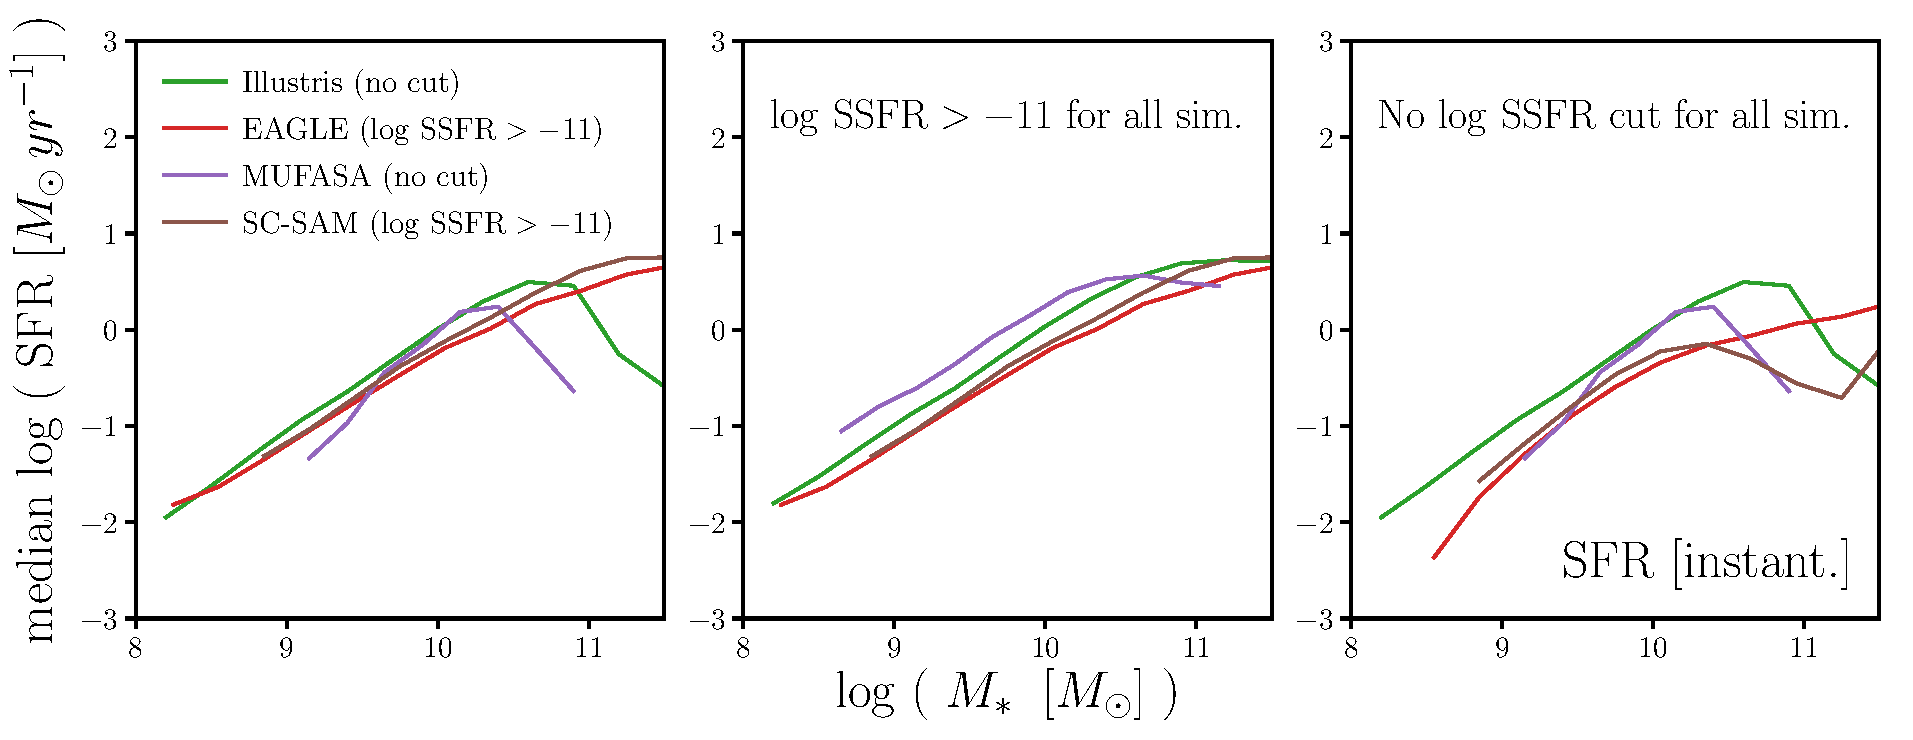
\includegraphics[width=0.75\textwidth]{Catalog_SFS_lit.pdf} 
\caption{\bf \color{red} The SFSs of Illustris, EAGLE, {\sc Mufasa}, 
and SC-SAM central galaxies, where we measure the SFSs using 
different methods as in Figure 5  of \cite{somerville2015} (left panel) 
and using the same methods (center and right panels). In the left panel, 
we measure the SFSs by taking the median SFR in  a $M_*$ bin with no 
selection cuts for Illustris and {\sc Mufasa} and by taking the median 
SFR after a SSFR > $10^{-11}\, \mathrm{yr}^{-1}$ cut for EAGLE and SC-SAM. 
In the center panel, we measure the SFSs by taking the median SFR after 
a SSFR > $10^{-11}\,\mathrm{yr}^{-1}$ cut for all four simulations. 
In the right panel, we measure the SFSs by taking the median SFR with 
no selection cuts for all four simulations. The difference among the 
panels illustrate that \emph{the agreement found in the left panel, 
and similarly in \cite{somerville2015}, is mainly driven by the 
difference in methods used to measure SFSs.}} 
\label{fig:likeSD14}
\end{center}
\end{figure*}
%%%%%%%%%%%%%%%%%%%%%%%%%%%%%%%%%%%%%%%%%%

In the left panel of Figure~\ref{fig:likeSD14} we reproduce the SFS comparison of 
\cite{somerville2015} Figure 5 for the simulations in Section~\ref{sec:galsims}
using different methods for measuring the SFS. For Illustris and EAGLE, we apply
the same methods as the SFSs in \cite{somerville2015}: 
the median SFR in a $M_*$ bin with no selection cut for Illustris (green) and 
with a SSFR > $10^{-11}\, \mathrm{yr}^{-1}$ cut for EAGLE~\citep[red;][]{schaye2015}. 
{\sc Mufasa} and the current version of SC-SAM did not exist and were not 
included in \cite{somerville2015}. Since we are illustrating how inconsistent 
SFS measurements can result in misleading agreement, for {\sc Mufasa} and 
SC-SAM we measure the median SFR with no selection cut and with a SSFR > 
$10^{-11}\, \mathrm{yr}^{-1}$ cut, respectively. As in Figure 5 of \cite{somerville2015}, 
we find good agreement among the SFSs of the simulations. 

{\bf \color{red} Instead of measuring the SFSs differently, if we measure the SFS 
by taking the median SFR after either a SSFR > $10^{-11}\, \mathrm{yr}^{-1}$ cut 
or  with no SSFR cut consistently for all the  simulations, we find discrepancies 
in the SFSs on the order of ${\sim}0.5\,\mathrm{dex}$ (center and right panels of \ref{fig:likeSD14}).
} 
This illustrates that the agreement found in 
\cite{somerville2015} is driven in large part by the difference in methods used to 
measure SFSs. 
{\bf \color{red}
Furthermore, the difference between the Illustris and {\sc Mufasa} SFSs in 
the panels illustrate how different SFS fitting methods, even when 
consistently applied, can alter the difference between SFSs. The difference 
between the Illustris and {\sc Mufasa} SFSs is significantly larger in the 
center panel when the SSFR > $10^{-11}\, \mathrm{yr}^{-1}$ cut is applied and 
galaxies with SFR below the resolution limit, which make up a larger fraction of the {\sc Mufasa} 
galaxies than the Illustris galaxies, are removed by the selection cut. In 
the center panel of Figure~\ref{fig:likeSD14}, we find consistency among the
slopes of the different SFSs. This consistency is a result of the hard selection 
cut, which biases the SFS slopes closer to the cut (SSFR = $10^{-11}\, \mathrm{yr}^{-1}$)
and thus to one another. These effects highlight the impact of hard selection scuts 
and the need for a consistent data-driven method for identifying the SFS that 
better account for intrinsically different SFR--$M_*$ distributions in the simulations.} 
%Therefore, Figure~\ref{fig:likeSD14} highlights the impact  of hard selection cuts and the importance of using a consistent data-driven  methodology for measuring the SFS. 

%Furthermore, Figure~\ref{fig:likeSD14} highlights the impact of hard selection cuts  and the importance of using a consistent methodology for measuring the SFS. 

%In this paper we perform a Gaussian Mixture Model fitting of the SFR-$M_{\star}$ plane and find almost an order of magnitude discrepancy in normalization of the Star Formation Sequence when described by the peak of our most dominant Gaussian component. This is seemingly in contrast to results from the literature that report agreement between simulations and observations ~\citep[\emph{e.g.}][]{ 
%somerville2015, genel2014, sparre2015, schaye2015, bluck2016, dave2016}. This apparent "disagreement" between our and previous results is mostly due to whether the authors applied a cut to select star-forming galaxies before fitting the SFS or not. Arguments can be found for both sides: fitting the SFS using only galaxies above a minimum sSFR or fitting the SFS using all galaxies. Additional disagreement exists in whether to use means, or medians, or when applying a cut-off what that should be. In Fig. \ref{fig:likeSD14} we show an identical figure to the comparison figure (Fig. 5) in \citet{somerville2015} where we apply almost exactly the same selection as the modelers did for that figure for Illustris and EAGLE (we chose a cut of sSFR > $-11$ yr$^{-1}$ instead of the sSFR > $-10.5$ yr$^{-1}$ used in \citet{schaye2015}). Both MUFASA and the current version of the SCSAM were not in existence at the time and for those we chose to either select star-forming galaxies (using a cut of sSFR > $-11$ yr$^{-1}$) or all galaxies, whichever fit best to the Illustris and EAGLE results. The caption of Fig. 5 in \citet{somerville2015} noted that "some of the modelers have applied a cut to select star forming galaxies, but some have not". As is shown in that figure and Fig. \ref{fig:likeSD14}, the simulations agree very well on the slope and normalization of the SFS. 
%However, when we choose to either select the star forming galaxies or all galaxies for all simulations the results are quite different. This can be seen in Fig. \ref{fig:medianSFall}. In both cases selecting the same sample of galaxies results in a disagreement in the normalization of the SFS of > 0.5 dex. This is the main driver of the disagreement that we found in this paper. Additional differences can arise in our method because a GMM models both the peak and the width of the SFS and is more sensitive to the position of the green valley with respect to the SFS. Additionally applying GMM results in intermediate or transitioning and starburst components when those populations are statistically significant. While we also use only central galaxies and apply a group finder to select those centrals, these effects are very minor. 

\section{Identifying the SFS using Gaussian Mixture Models} \label{app:gmm_pssfr}
In order to derive the best-fit GMM used for identifying the SFS in 
each $M_*$ bin, we compare GMM fits with $k\leq 3$ components using
their BICs (Section~\ref{sec:sfmsfit}). In Figures~\ref{fig:pssfr_gmm_inst} 
and~\ref{fig:pssfr_gmm_100myr}, we illustrate this comparison among the  
GMMs with $k=1, 2,$ and $3$ (blue, orange, and green) components fit
to the instantaneous SSFR distributions, $P(\log\,\mathrm{SSFR})$, of the 
Illustris, EAGLE, {\sc Mufasa}, and SC-SAM (top to bottom panels) centrals 
in three stellar mass bins: 
$9.2 <\log\,M_*<9.4$, $9.8 <\log\,M_*<10$, and $10.6 <\log\,M_*<10.8$ (left to right). 
The SSFR distributions in Figures~\ref{fig:pssfr_gmm_inst} 
and~\ref{fig:pssfr_gmm_100myr} are derived using instantaneous and 
$100\,\mathrm{Myr}$ SFRs respectively. Galaxies with unmeasurably low SFR %$\mathrm{SFR}{=}0$
are represented at the edge of the SSFR distributions with $\log\,\mathrm{SSFR}=-13.5$.
In each panel, we also present the BICs and plot every component of the 
GMM fits (dashed) in their respective colors. These figures illustrate
the advantages of the data-driven GMM based fitting and BIC based
model selection used in our SFS fitting.

%%%%%%%%%%%%%%%%%%%%%%%%%%%%%%%%%%%%%%%%%%
% Figure 
%%%%%%%%%%%%%%%%%%%%%%%%%%%%%%%%%%%%%%%%%%
\begin{figure*}
\begin{center}
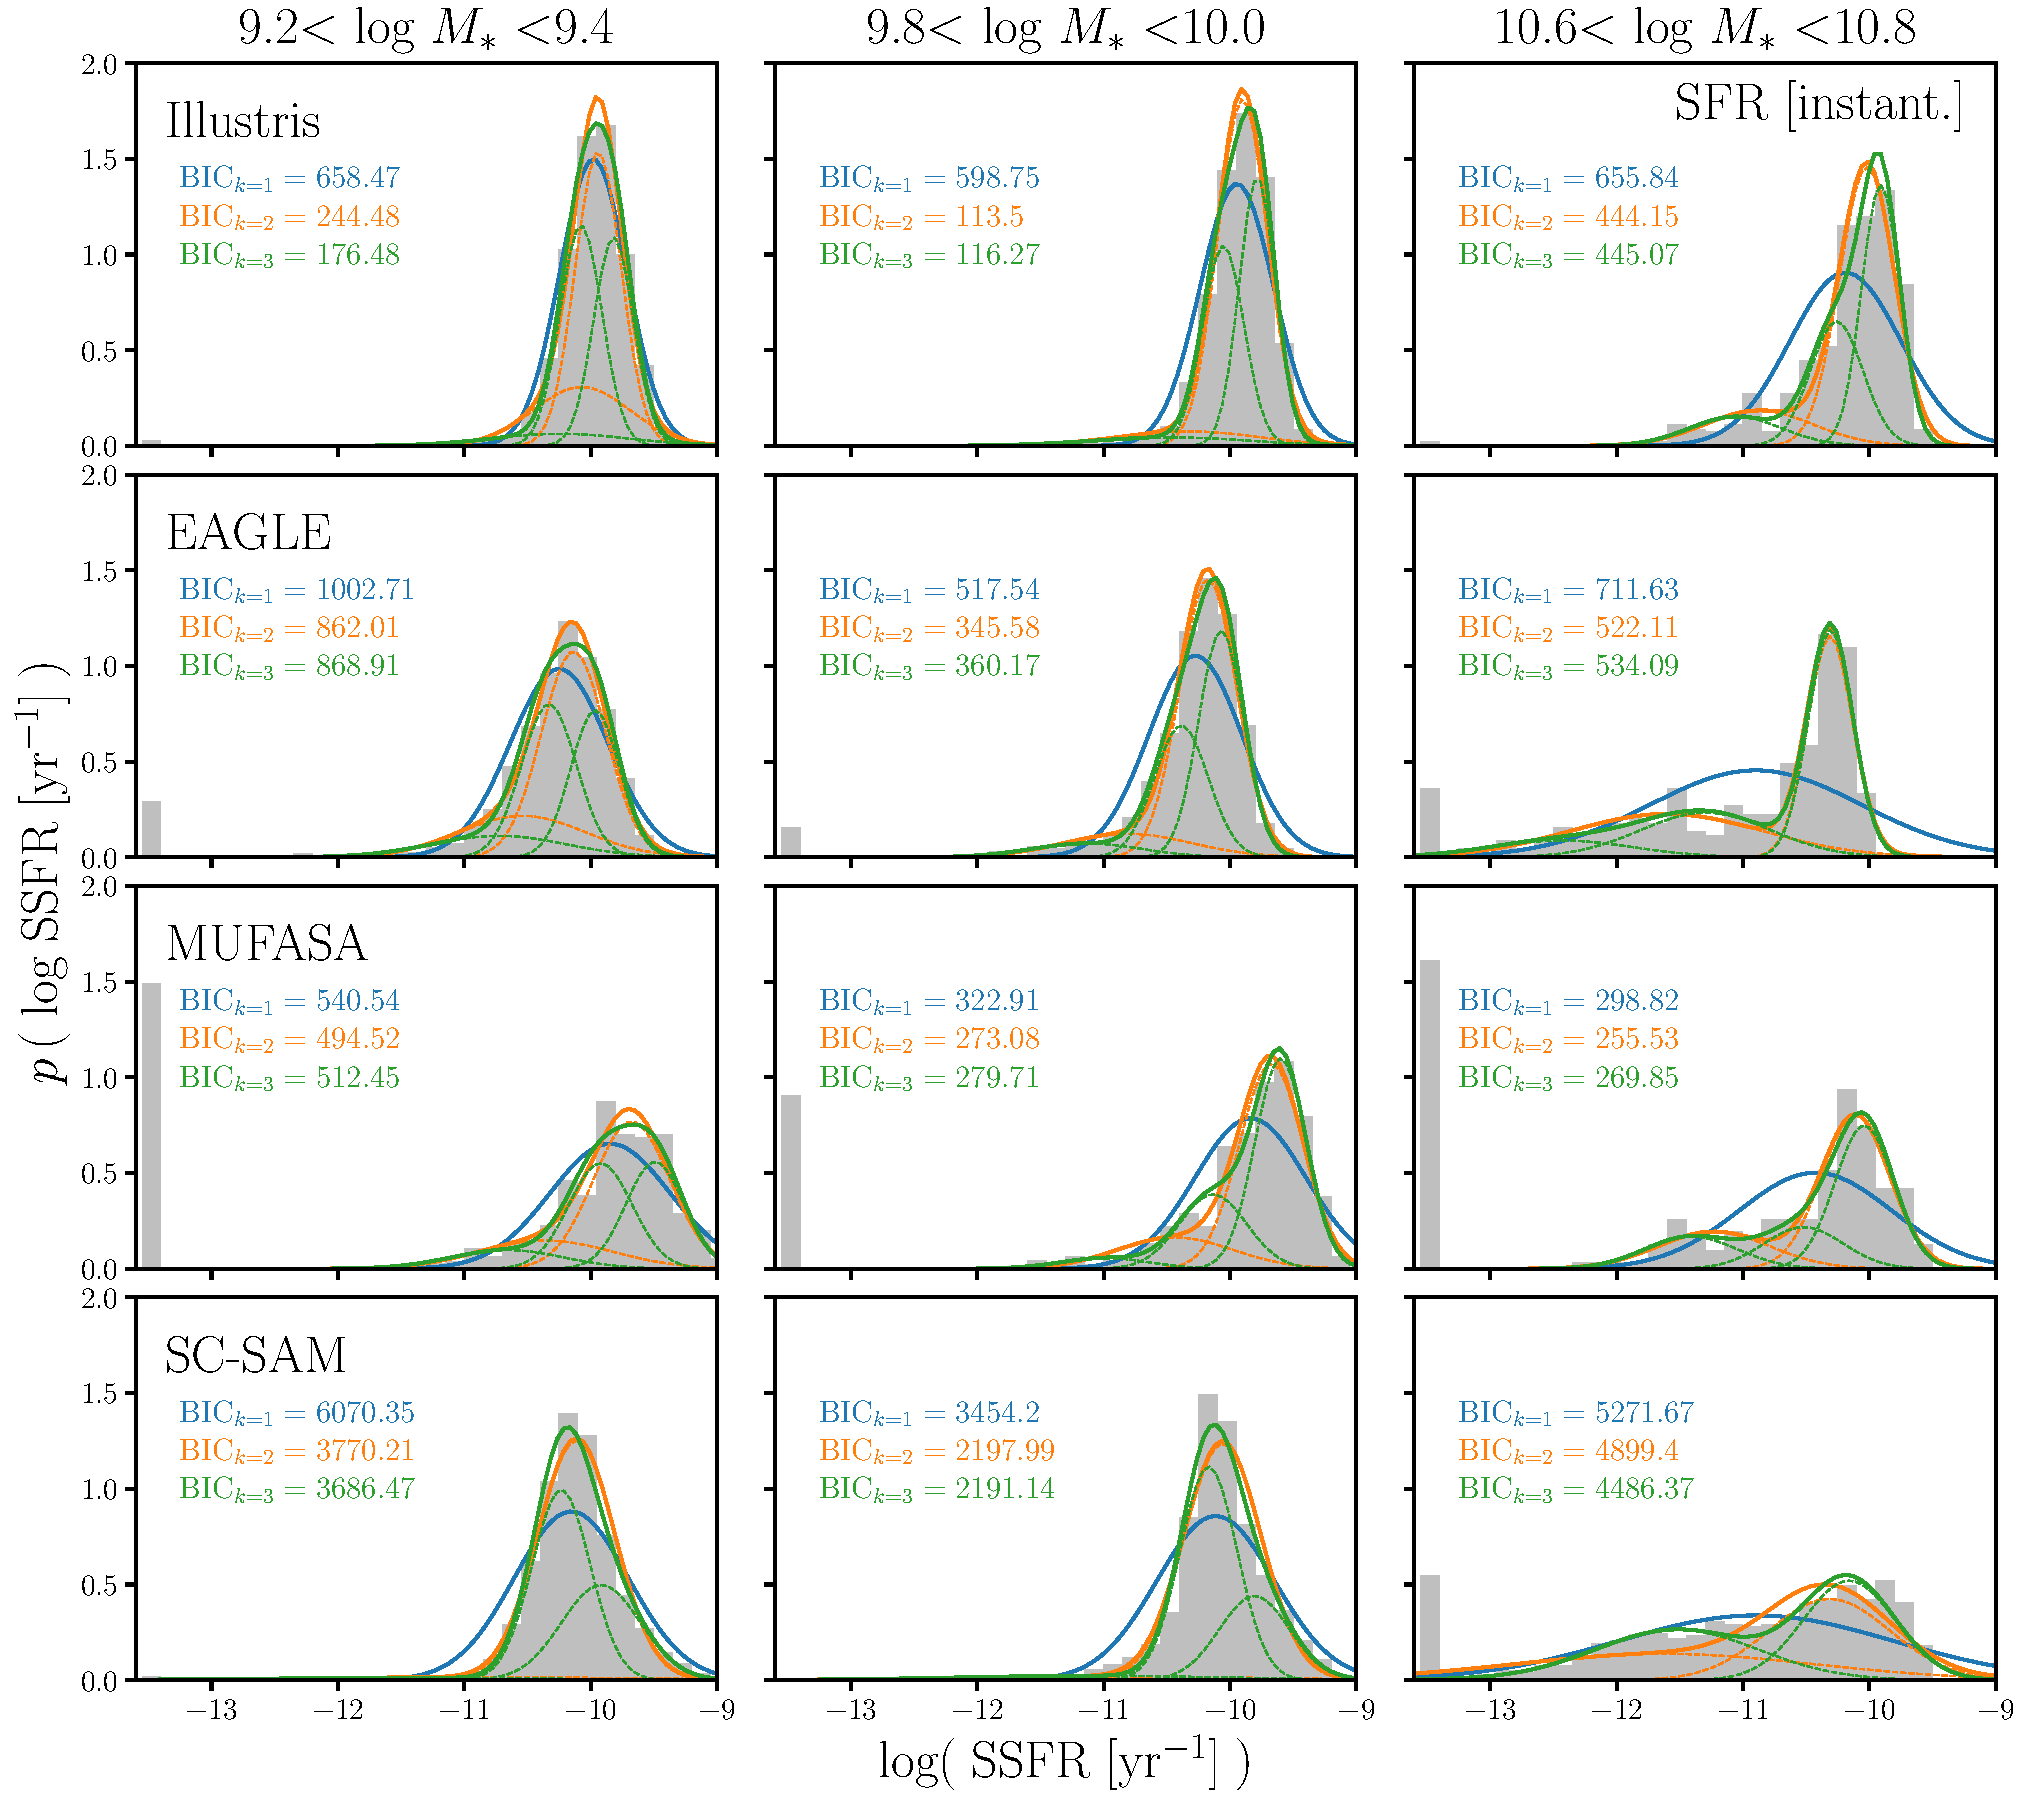
\includegraphics[width=0.95\textwidth]{Pssfr_GMMcomps_inst.pdf} 
\caption{GMMs with $k=1, 2,$ and $3$ (blue, orange, and green) components fit
to the instantaneous SSFR distributions, $P(\log\,\mathrm{SSFR})$, of the 
Illustris, EAGLE, {\sc Mufasa}, and SC-SAM (top to bottom panels) centrals 
in three stellar mass bins: $[9.2, 9.4]$, $[9.8, 10.]$, and $[10.6, 10.8]$ 
(left to right). We represent galaxies with unmeasurably low SFR in 
$P(\log\,\mathrm{SSFR})$s with $\log\,\mathrm{SSFR} = -13.5$. 
For every GMM fit, we plot each component in dash lines 
and list their BICs in the same color. In our SFS fitting, we select the 
GMM with the lowest BIC as the best-fit. This provides a \emph{data-driven 
way of accurately fitting the SSFR distribution while avoiding overfitting}.
} 
\label{fig:pssfr_gmm_inst}
\end{center}
\end{figure*}
%%%%%%%%%%%%%%%%%%%%%%%%%%%%%%%%%%%%%%%%%%
%%%%%%%%%%%%%%%%%%%%%%%%%%%%%%%%%%%%%%%%%%
% Figure 
%%%%%%%%%%%%%%%%%%%%%%%%%%%%%%%%%%%%%%%%%%
\begin{figure*}
\begin{center}
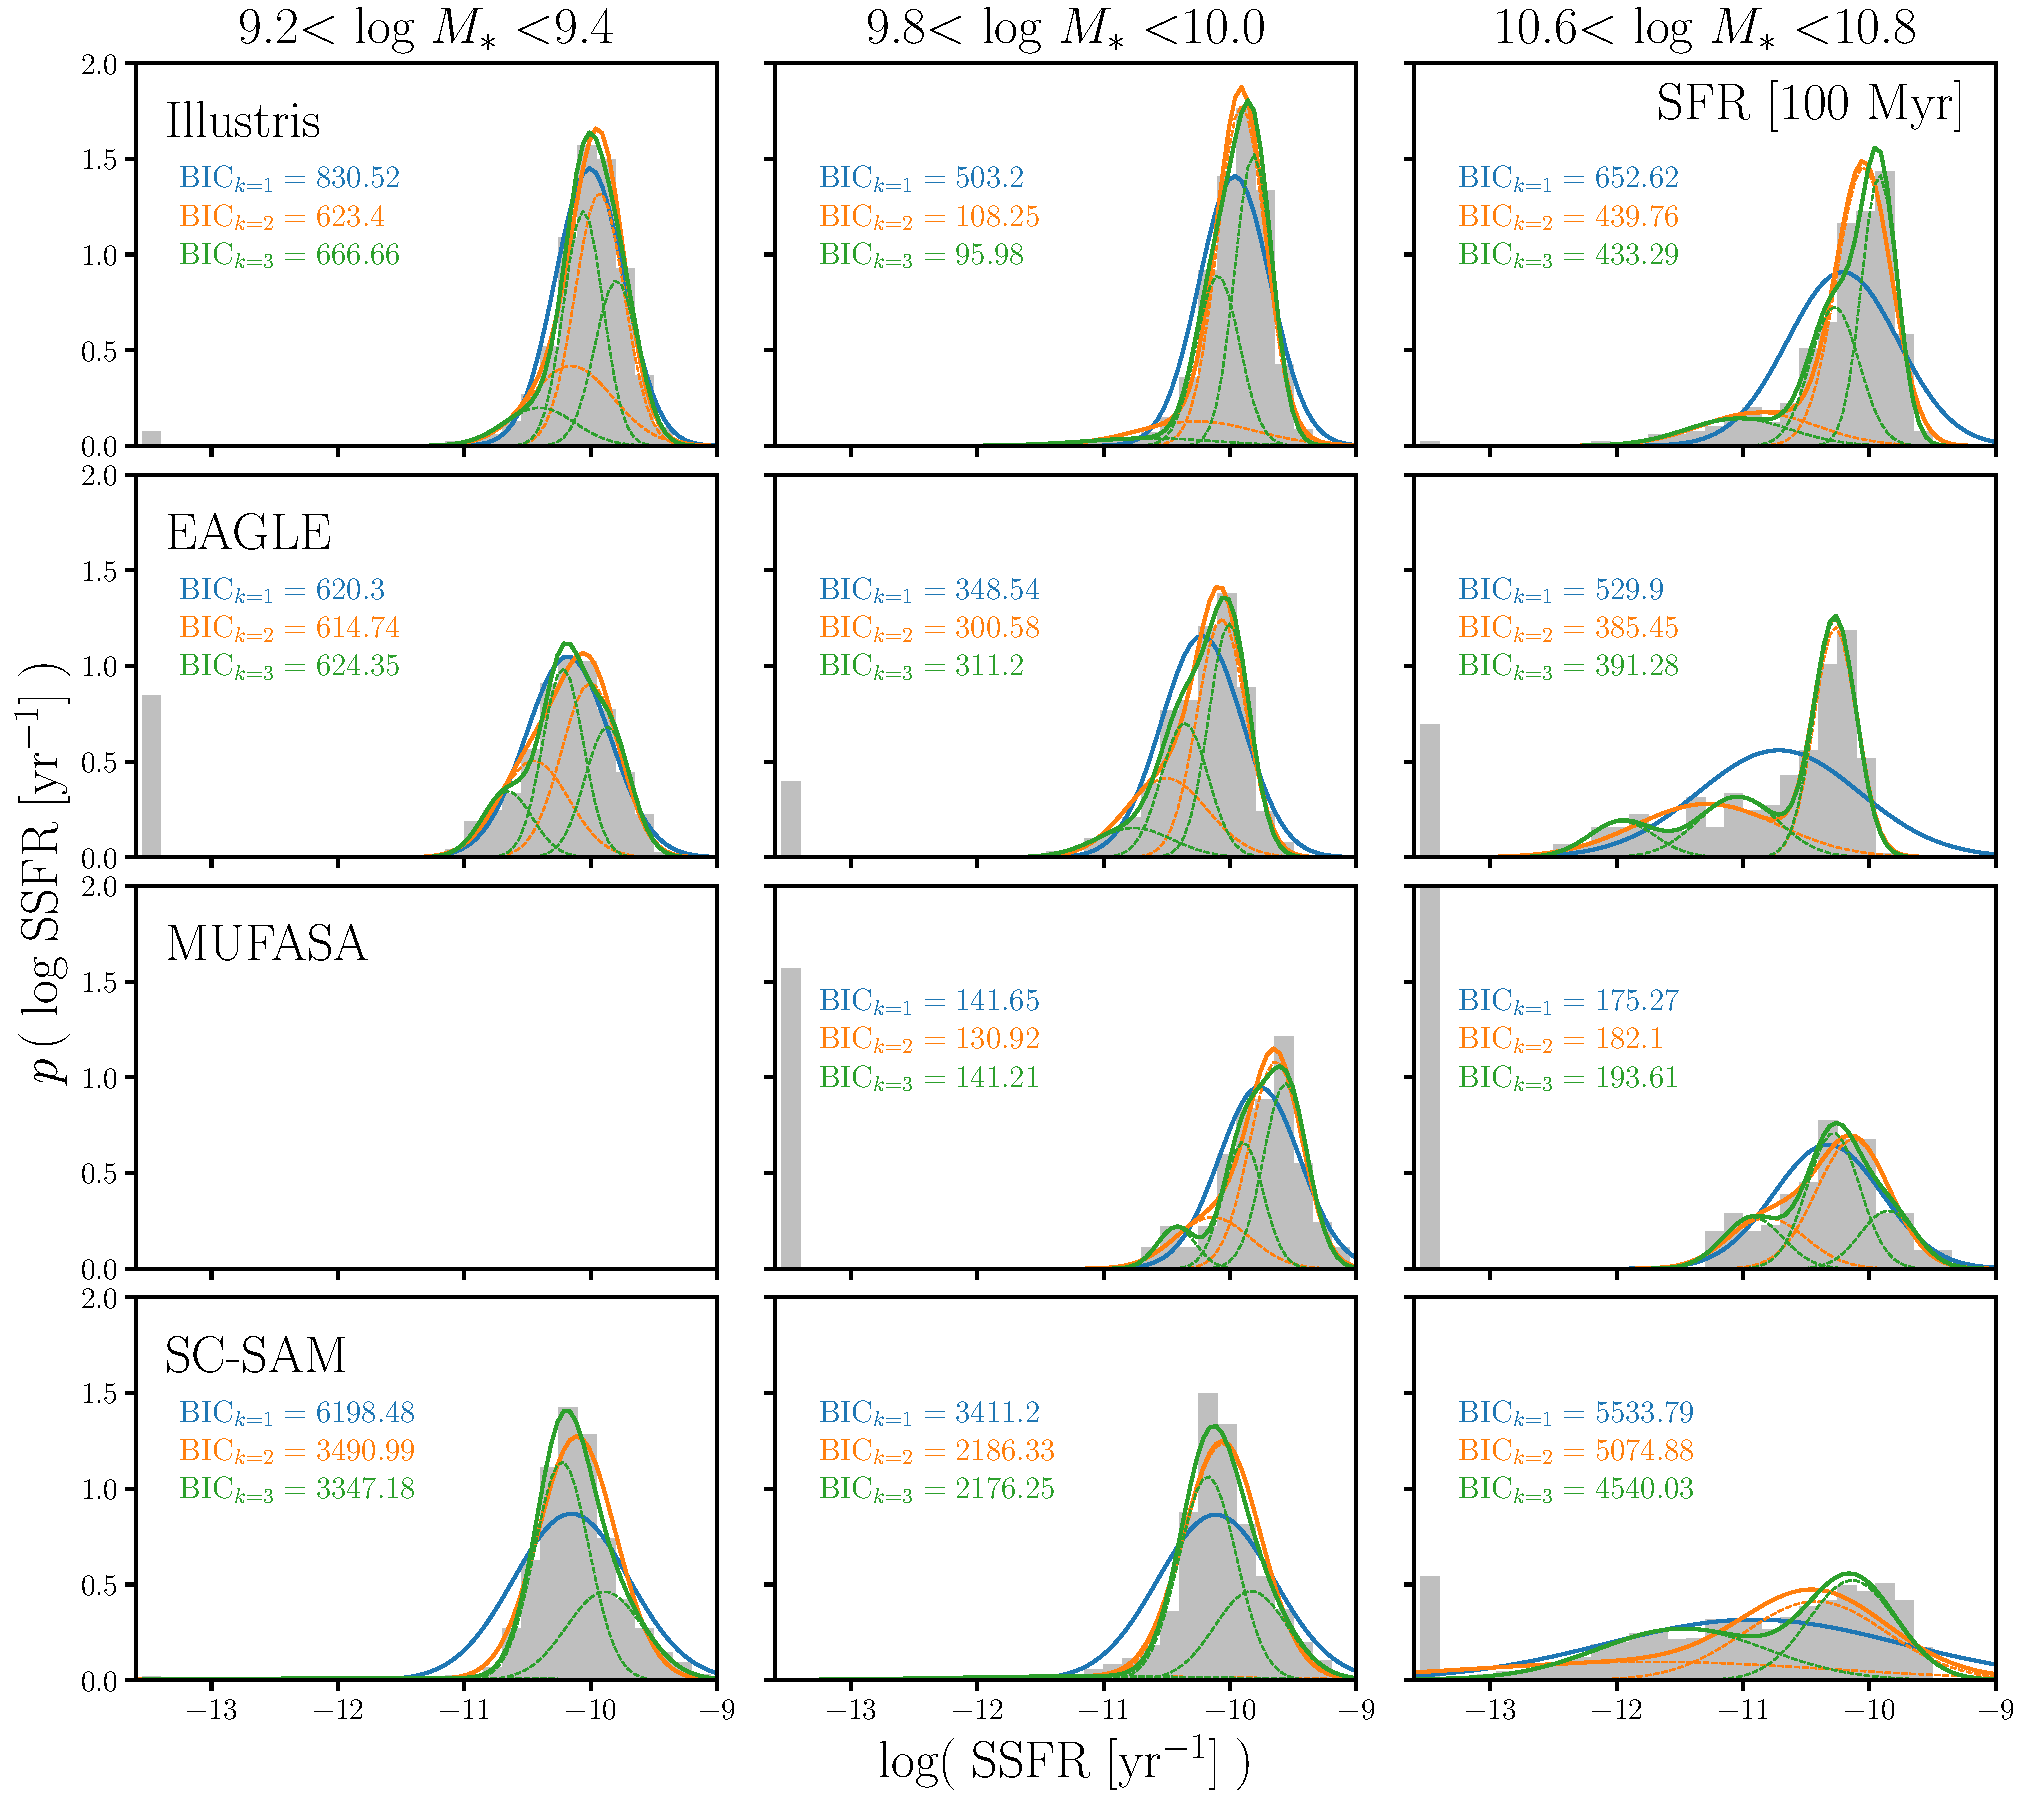
\includegraphics[width=0.8\textwidth]{Pssfr_GMMcomps_100myr.pdf} 
\caption{Same as Figure~\ref{fig:pssfr_gmm_inst} but for the $100\,\mathrm{Myr}$
SSFR distributions.} 
\label{fig:pssfr_gmm_100myr}
\end{center}
\end{figure*}
%%%%%%%%%%%%%%%%%%%%%%%%%%%%%%%%%%%%%%%%%%
For instance, in most of the highest $M_*$ bin (right panels in both figures) 
the $k=1$ GMM fits do not reflect the clearly bimodal SSFR distributions.
In these cases, the $\mathrm{BIC}_{k=1}$ is significantly larger than
$\mathrm{BIC}_{k=2}$ and $\mathrm{BIC}_{k=3}$, so our BIC based model 
selection favors GMMs with more than one component. In fact, GMMs with
more components are more flexible and generally can better fit the underlying 
distribution. However as the EAGLE and {\sc Mufasa} $9.8 <\log\,M_*<10$ 
bins of the figures illustrate, our BIC based model selection does not 
always favor the higher $k$ GMM fits. Although the $k=3$ GMMs have the 
lowest $\chi^2$ in these panels, because of the penalty term for the 
number of model parameters, our BIC criteria favors the $k=2$ GMMs.
According to the BICs, the $k=3$ GMMs in these panels overfit the 
SSFR distributions.
{\bf \color{red} 
The figures also illustrate that among the GMM fits with comparably 
low BICs, the dominant component that describe the star-forming portion 
of $P(\log\,\mathrm{SSFR})$ is {\em not} significantly impacted. Since 
this component is mainly identified as the SFS, our BIC based model
selection does not strongly impact the position and width of the SFS.  
}

%In a number of stellar mass bins, the best-fit GMMs have more than one 
%$\log\,\mathrm{SSFR} > -11$ components. In these cases the 
%$\log\,\mathrm{SSFR} > -11$ component with the highest weight is identified
%as the SFS component (Section~\ref{sec:sfmsfit}). 

From the best-fit GMMs, we identify the SFS components iteratively starting 
from the lowest $M_*$ bin as described in Section~\ref{sec:gmm}. We 
consider other components, depending on their mean, as low, intermediate, or high 
SF components in Section~\ref{sec:beyondsfms}. The SC-SAM in particular has 
high SF components at $M_* \lesssim 10^{10}M_\sun$ (bottom left and center 
panels of Figures~\ref{fig:pssfr_gmm_inst}  and~\ref{fig:pssfr_gmm_100myr}).
In these cases, the SSFR distribution is not well described by a single log-normal distribution.
{\bf \color{red}
Instead the distribution is significantly asymmetric with a 
heavier tail on the more star-forming end of the distribution. 
An extra component to account for the non-Gaussianity improves 
the fit more than the penalty term, giving us the high SF components.
Our method for identifying the SFS and other components using GMMs 
assumes that the components are Gaussian. However, from the data 
alone, it is impossible to determine the shape of the ``true'' 
galaxy sub-population distributions. While mixture models with 
non-Gaussian components can be used instead, without knowing the 
``true'' sub-populations, they will still require assumptions on 
the shape of the components. Therefore, in Section~\ref{sec:beyondsfms} 
when we discuss components besides the SFS (low, intermediate, and high), 
we distinguish between the components and the galaxy sub-populations 
commonly referred to in the literature (quiescent, transitioning and 
starburst). 
}

%So far we have assumed that one, two, or three populations would describe galaxies in the SFR--$M_*$ plane well. We have checked whether the possibility of adding more than three Gaussians in the GMM shows that more populations are present. This is the case only for the Santa Cruz semi-analytic model, where in a number of bins the presence of 4, 5, or (in one case) 6 Gaussians is preferred. In almost all cases the added Gaussians have low weight and form effectively additional intermediate populations. For both Illustris and EAGLE there is only one mass bin where a fourth population would be preferred. For all other mass bins in all the hydrodynamic simulations, and all mass bins in the SDSS 3 or less Gaussians are preferred.

%In addition to identifying the SFS, the GMM fitting method described above can  be extended to describe the entire SFR-$M_*$ relation using a two-dimensional  GMM. In Figure~\ref{fig:2dgmm}, we compare the instantaneous SFR to $M_*$ relation  of central galaxies in the EAGLE simulation with the best-fit two-dimensional GMM.  The over-plotted shaded ellipses represent the two-dimensional Gaussian components of the best-fit GMM. Overall the best-fit 2D GMM captures the features in the  EAGLE SFR-$M_*$ relation. It also provides a straightforward way of comparing  different SFR-$M_*$ relations. However, as Figure~\ref{fig:2dgmm} illustrates,  specifically identifying the SFS using the two-dimensional model is more  challenging. Therefore in this paper, we do not discuss the 2D GMM further. 
\section{Resolution Effects in Hydrodynamic Simulations} \label{app:zerosfr}
In our analysis, we consistently derive SFRs for all of the simulated
galaxies on two timescales: instantaneous and averaged over 
$100\,\mathrm{Myr}$ (Section~\ref{sec:galsims}). For the hydrodynamic 
simulations, SFR averaged over $100\,\mathrm{Myr}$ is derived using 
the formation times of the star particles in the simulation, which 
means that the mass and temporal resolutions of the simulations 
impact the $100\,\mathrm{Myr}$ SFR. In Illustris, EAGLE, and {\sc Mufasa},
their $100\,\mathrm{Myr}$ SFRs have resolutions of 
$\Delta_\mathrm{SFR} = 0.0126$, $0.018$, and $0.182\,M_\sun \mathrm{yr}^{-1}$, 
corresponding to baryon particle masses of $1.26 \times 10^6\ M_{\sun}$, 
$1.8 \times 10^6\ M_{\sun}$, and $1.82 \times 10^7\ M_{\sun}$, respectively. 
For SFR averaged over $10\,\mathrm{Myr}$, the $\Delta_\mathrm{SFR}$s would be 
10 times larger. Therefore, we instead use instantaneous SFRs to measure 
star formation on the shortest timescale.

%%%%%%%%%%%%%%%%%%%%%%%%%%%%%%%%%%%%%%%%%%
% Figure 
%%%%%%%%%%%%%%%%%%%%%%%%%%%%%%%%%%%%%%%%%%
\begin{figure*}
\begin{center}
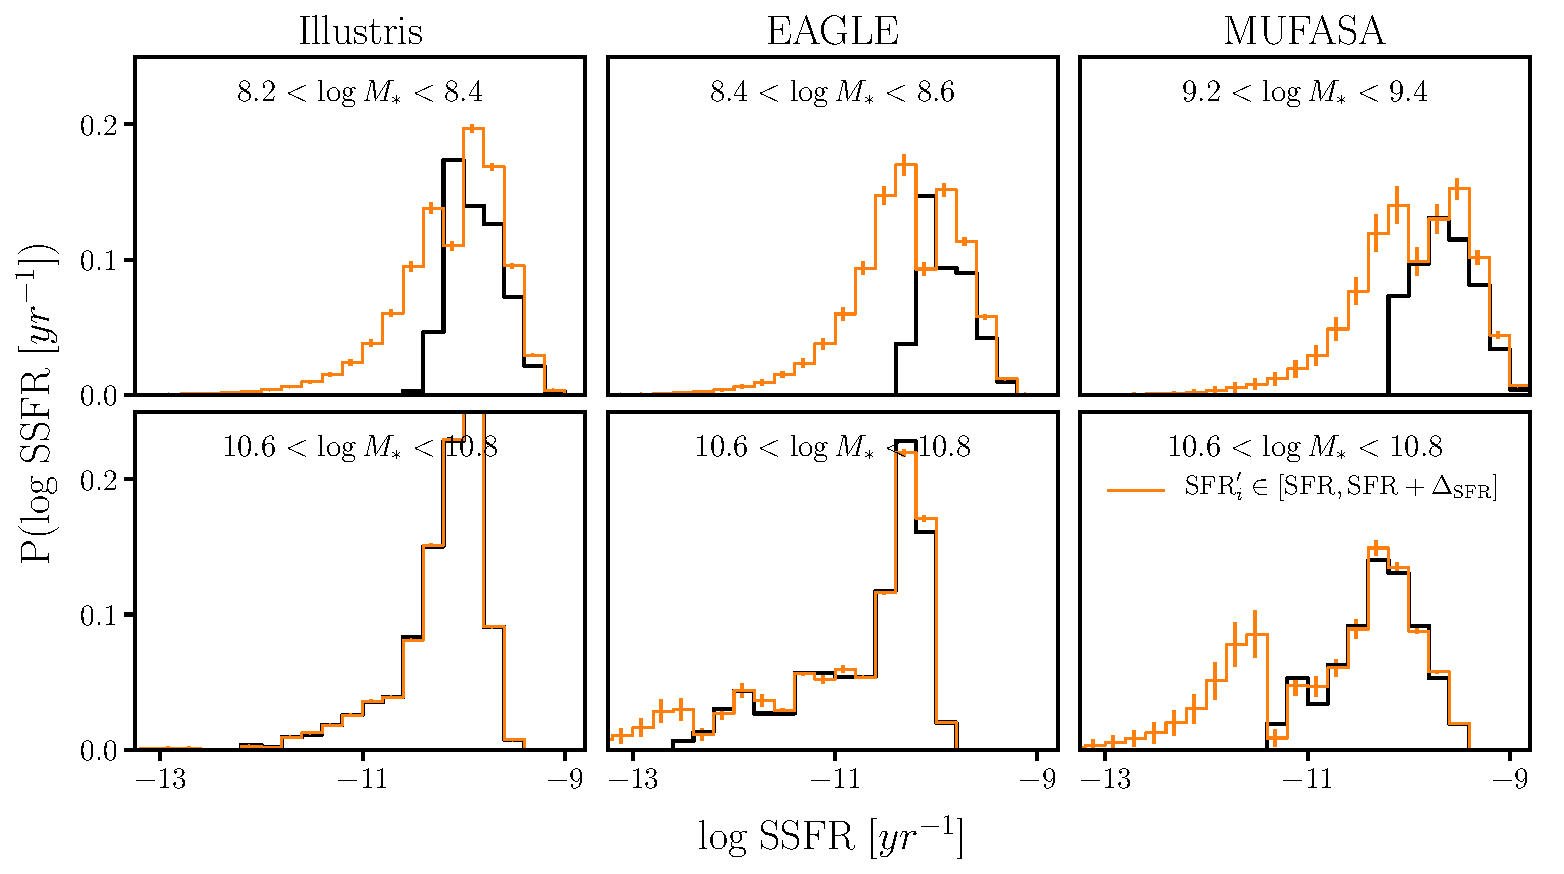
\includegraphics[width=0.7\textwidth]{Pssfr_res_impact.pdf} 
\caption{The impact of SFR resolution on the SSFR distribution, 
$P(\log\,\mathrm{SSFR})$, in two stellar mass bins of the hydrodynamic 
simulations:
Illustris (left), EAGLE (center), and {\sc Mufasa} (right). We plot the 
$P(\mathrm{SSFR})$ distributions using the $100\,\mathrm{Myr}$
SFRs \emph{with} resolution effects in black. These exclude galaxies with 
unmeasurably low SFRs. In orange, we plot the $P(\log\,\mathrm{SSFR})$ 
distributions where the SFRs of the galaxies
are sampled uniformly within the SFR resolution range 
($[\mathrm{SFR}_i, \mathrm{SFR}_i+\Delta_\mathrm{SFR}]$). The 
uncertainties for the orange $P(\mathrm{SSFR})$s are estimated from 
re-sampling the SFR of each galaxy based on the SFR resolution. 
At low stellar masses (top) the SFR resolution significantly impacts 
the star-forming end of $P(\mathrm{SSFR})$s. At higher stellar masses, 
although the SFR resolution impacts the $P(\mathrm{SSFR})$s, the effect 
is limited to below $\log\,\mathrm{SSFR} < -11$.
} 
\label{fig:sfrres_pssfr}
\end{center}
\end{figure*}
%%%%%%%%%%%%%%%%%%%%%%%%%%%%%%%%%%%%%%%%%%

% describe the impact of resolution effect more concretely 
For galaxies with high $100\,\mathrm{Myr}$ SFR, the resolution 
$\Delta_\mathrm{SFR}$ is relatively small compared to their SFRs and
therefore it does not have a significant impact. However for low SFR 
galaxies, the resolution effect is more significant. At the lowest SFR 
end, galaxies that, without the resolution effect, would have SFR ranging 
$0 < \mathrm{SFR} < \Delta_\mathrm{SFR}$, may have unmeasurably low SFR 
($\mathrm{SFR}{=}0$) with the resolution effect. These galaxies are thereby 
not included in the $\mathrm{SFR}$--$M_*$ plane or when we identify the SFS. In
Figure~\ref{fig:sfrres_pssfr}, we present the impact of excluding these
galaxies and the overall resolution effect on the $P(\log\,\mathrm{SSFR})$ 
distributions of the hydrodynamic simulations in two stellar mass bins. In 
black, we plot the $P(\log\,\mathrm{SSFR})$ distributions using the 
$100\,\mathrm{Myr}$ SFRs \emph{with} resolution effects
(\emph{excluding} galaxies with unmeasurably low SFR). In orange, we plot the 
$P(\log\,\mathrm{SSFR})$ distributions of \emph{all} galaxies where
$\mathrm{SFR}'_i$ of each galaxy sampled uniformly within the SFR resolution range, 
$[\mathrm{SFR}_i, \mathrm{SFR}_i+\Delta_\mathrm{SFR}]$. Uncertainties 
for the orange $P(\log\,\mathrm{SSFR})$s are derived from repeating this 
SFR sampling $100$ times. For the low $M_*$ bins (top), the SFR resolution 
affects the $P(\log\,\mathrm{SSFR})$s well above $\log\,\mathrm{SSFR}{=}{-}11.0$ 
on the star-forming end of the distribution. Meanwhile, the impact at higher
$M_*$ (bottom), is limited to the low SSFR end. 

%%%%%%%%%%%%%%%%%%%%%%%%%%%%%%%%%%%%%%%%%%
% Figure 
%%%%%%%%%%%%%%%%%%%%%%%%%%%%%%%%%%%%%%%%%%
\begin{figure*}
\begin{center}
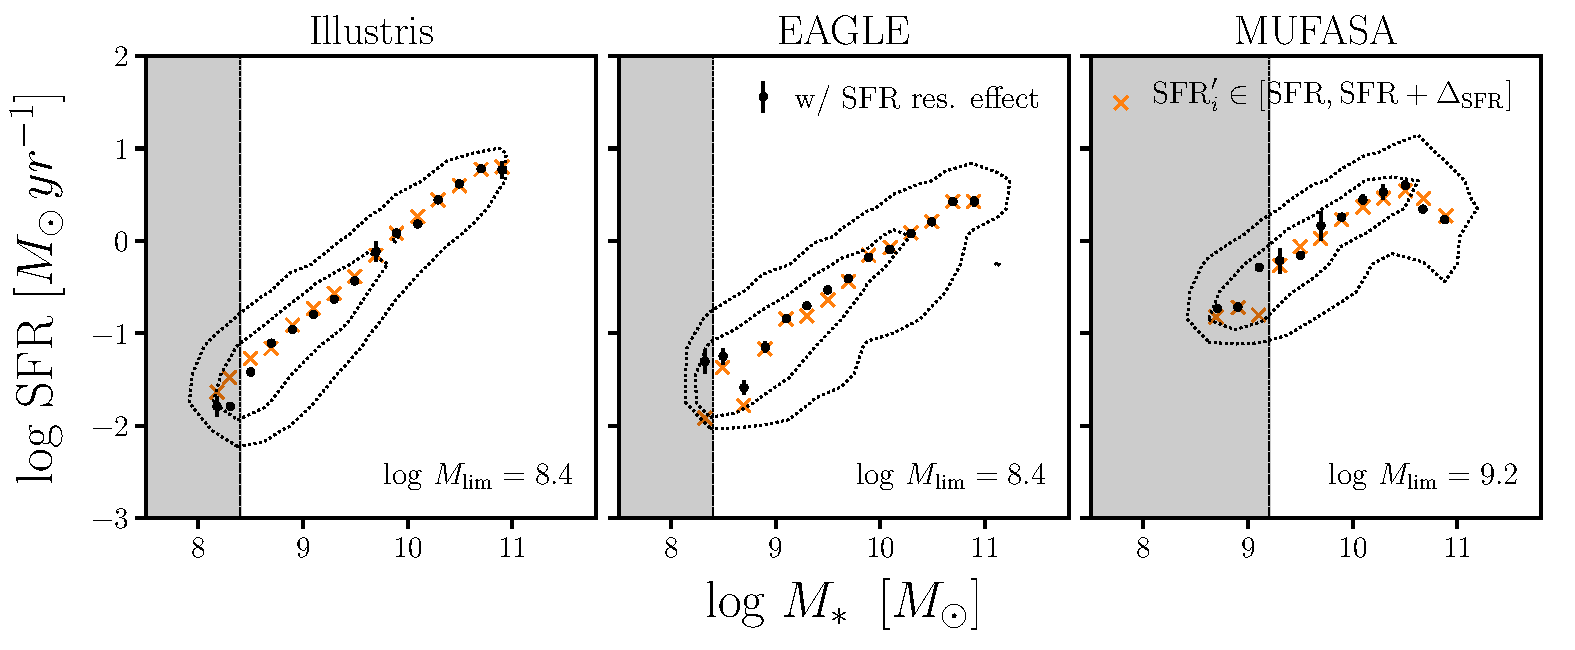
\includegraphics[width=0.75\textwidth]{Mlim_res_impact.pdf} 
\caption{The resolution effect of $100\,\mathrm{Myr}$ SFRs in the hydrodynamic 
simulations (Illustris, EAGLE, and {\sc Mufasa}) impact the identified SFSs 
at low stellar masses. In black we plot the best-fit SFS 
with the resolution effects. In orange we plot the best-fit SFS where 
the SFR for each galaxy is sampled uniformly within the resolution range: 
$\mathrm{SFR}_i^{\prime} \in [\mathrm{SFR}_i, \mathrm{SFR}_i +
\Delta_\mathrm{SFR}]$). Based on the discrepancy between the fits, we determine 
stellar mass limits above which the SFR resolution does {\em not} 
significantly impact ($< 0.2\,\mathrm{dex}$) the identified SFS. For Illustris, 
EAGLE, and {\sc Mufasa} this corresponds to $\log M_\mathrm{lim} = 8.4, 8.4$, 
and $9.2$, as shown in the gray shaded region.} 
\label{fig:mlim_res}
\end{center}
\end{figure*}
%%%%%%%%%%%%%%%%%%%%%%%%%%%%%%%%%%%%%%%%%%
In order to better quantify the impact of the SFR resolution effect
on our SFS fitting, in Figure~\ref{fig:mlim_res} we compare the SFS fits 
using $100\,\mathrm{Myr}$ SFRs \emph{with} resolution effects (black) to 
the SFS fits using $100\,\mathrm{Myr}$ SFRs sampled uniformly within the 
SFR resolution range (orange; 
$\mathrm{SFR}_i^{\prime} \in [\mathrm{SFR}_i, \mathrm{SFR}_i + \Delta_\mathrm{SFR}]$). 
The uncertainties of our SFS fits in black are calculated using bootstrap 
resampling (Section~\ref{sec:sfmsfit}). In agreement with 
Figure~\ref{fig:sfrres_pssfr}, we find that the SFR resolution 
significantly impacts the identified SFS at low $M_*$. Moreover, using the 
comparison of Figure~\ref{fig:mlim_res}, we determine the stellar mass 
limit above which the SFR resolution does {\em not} significantly impact 
the identified SFS --- \emph{i.e.} the shift in best-fit SFS is below 
$0.2\,\mathrm{dex}$. For Illustris, EAGLE, and {\sc Mufasa} we determine 
$\log M_\mathrm{lim} = 8.4, 8.4$, and  $9.2$, respectively. For EAGLE, 
where we have a higher resolution box ($8\times$ higher baryon mass 
resolution) available, we further confirm that the SFS is not significantly 
impacted above $\log M_\mathrm{lim}$.

%%%%%%%%%%%%%%%%%%%%%%%%%%%%%%%%%%%%%%%%%%
% Figure 
%%%%%%%%%%%%%%%%%%%%%%%%%%%%%%%%%%%%%%%%%%
\begin{figure*}
\begin{center}
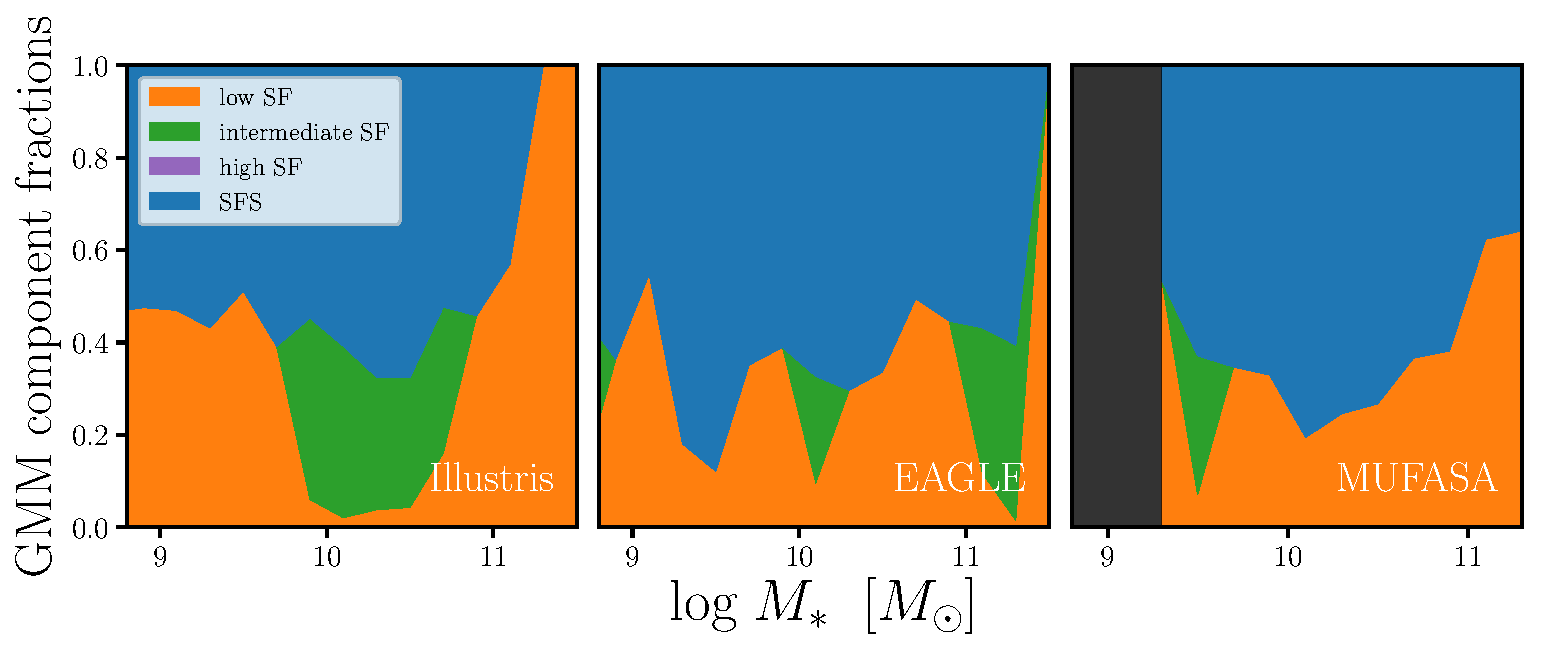
\includegraphics[width=0.7\textwidth]{GMMcomp_comp_res_impact.pdf}
\caption{Fractional contributions, $\pi_i$, of the best-fit GMM components 
from our method for the hydrodynamic simulations (Illustris, EAGLE, and 
{\sc Mufasa}) where we uniformly sample the $100\,\mathrm{Myr}$ SFRs within
the SFR resolution range --- $\mathrm{SFR}_i^{\prime} \in [\mathrm{SFR}_i, \mathrm{SFR}_i + 
\Delta_\mathrm{SFR}]$. Compared to Figure~\ref{fig:kandinsky}, we find SFR 
resolution has no significant impact on the qualitative results in Section~\ref{sec:beyondsfms}.} 
\label{fig:mlim_fcomp}
\end{center}
\end{figure*}
%%%%%%%%%%%%%%%%%%%%%%%%%%%%%%%%%%%%%%%%%%

In addition to its effect on the SFS fits, we also examine the impact of 
SFR resolution on our results regarding the non-SFS components of our GMM 
fitting (Figure~\ref{fig:kandinsky}). In 
Figure~\ref{fig:mlim_fcomp} we present the fraction contributions ($\pi_i$) 
of the best-fit components for the Illustris, EAGLE, and {\sc Mufasa} 
simulations, where we uniformly sample the SFRs within the SFR resolution 
range (same as above). Besides no longer having a component of galaxies 
with unmeasurably low SFRs due to the SFR sampling, we find no significant 
change from the $\pi_i$ of Figure~\ref{fig:kandinsky} and,  thus, the results of Section~\ref{sec:beyondsfms}. 

{\bf \color{red} 
In addition to its impact on the SFRs, the mass resolution of the hydrodynamic 
simulations also impact the stellar masses of the simulations. We note that the stellar mass functions differ with resolution as shown in \citet{schaye2015, genel2014, dave2016}. To determine
whether mass resolution has a significant impact on the identified
SFS, we compare the SFS identified from our EAGLE simulation 
(Section~\ref{sec:galsims}) to SFS identified from higher mass resolution 
L0025N0752 EAGLE simulation~\citep{schaye2015}. The L0025N0752 simulation
has baryonic mass resolution of $2.26 \times 10^5 M_\odot$ ($8 \times$ 
higher than our EAGLE simulation). From the comparison, we find that 
the SFS is underestimated near the mass resolution in our lower resolution 
EAGLE simulation. However, this impacts the SFS by less than 
$0.2\,\mathrm{dex}$. Although higher resolution simulations for Illustris 
are not available, we also compare the SFS identified from our Illustris 
simulations with SFSs identified from lower resolution Illustris simulations 
($8\times$ and $64\times$ lower resolutions) and find qualitatively 
consistent results. Therefore, we find that the effect of mass resolution 
on the stellar masses in hydrodynamic simulations does not significantly 
impact the SFS identified in the simulations, especially above the stellar 
mass  limits of our analysis.
}

\bibliographystyle{aasjournal}
\bibliography{paper1}
\end{document}



\begin{comment} 
## Referee Report 
#### Reviewer's Comments:
The paper 'IQ-Collaboratory 1.1: the Star-Forming Sequence of Simulated Central
Galaxies' by Hahn et al. compares the star-forming sequence (SFS) between
various simulations and SDSS. The key aspect of the comparison is the usage of
Gaussian Mixture Models to identify the SFS. The paper is written well, and the
results are definitely interesting and important for the community. I therefore
recommend this paper after some moderate revision (see below). 

#### Major comments:
---
M.1. [x][Chang] The authors discuss in Appendix C resolution questions regarding the SFR
estimates. However, also the stellar masses themselves will not be fully
converged for different resolution levels of the different simulations. How can
the authors compare stellar mass estimates from simulations with different mass
resolution? For example, a given simulation (e.g., EAGLE) will lead to different
stellar masses depending on the mass resolution. The same is true for the other
hydro simulations. So, how can the stellar mass of a galaxy be compared
between two simulations with different mass resolutions?

> In order to test the impact of mass resolution, we use a higher mass 
resolution EAGLE simulation and compare the identified SFSs. We find 
that the SFS is underestimated near the mass resolution limit
for lower resolution boxes. However, this is not a significant effect
and impacts the SFS by less than 0.2 dex. Although higher resolution 
Illustris simulations are not available, we use lower resolution 
Illustris simulations to conduct the same comparison and find consistent
results. Therefore, the impact of mass resolution on the stellar masses 
of hydro simulations does not significantly impact the identified SFSs,
especially above the stellar mass limits of our analysis. We discuss 
this comparison in Appendix C.  

M.2. [x][Chang] How sensitive is the identification of the SFS to the 
0.5 dex value for the difference between the mean values? Can the authors 
please demonstrate that this value does not affect the SFS identification 
in any significant way?

> We choose 0.5 dex in order to relax any assumptions on the slope
of the SFS and also avoid misclassifying the quiescent population 
as SFS at the high mass end. The SFS identification, however, is 
not significantly impacted by the difference between the mean values
within the range 0.2 - 0.8 dex. We include this discussion in Section 3. 

M.3. [x][Chang] I understand the advantages of the Gaussian Mixture Models. However, 
can the authors please clarify a few things: 
-Why shall we assume that the distribution of the different populations in the
Mstar - SFR plane are indeed Gaussian? How good is this approximation? Can the
authors please quantify non-Gaussian contributions?
-If k=3 is a good fit (based on the BIC), what does it physically mean to have
three components? The authors give some lose definition like low-SF, med-SF,
high-SF. But how certain can we be sure that these are real different
subpopulations?

> Our method of identifying the SFS and other components using GMMs, 
does not assume that the population as a whole is Gaussian. With GMMs, 
we determine the combination of Gaussians that best reproduce the
distribution of the population without any assumptions on the shape
of the distribution. As a result, any significant non-Gaussianities 
in the distribution would result in a GMM with extra components that
better match the non-Gaussianities in the distribution. This is the
case, for instance, in the SC-SAM logM_*=9.2-9.4 bins of Figures B.1. 
and B.2. (bottom left) where the best-fit GMM consists of two 
star-forming components rather than one. Although the components of 
the GMM are assumed to be Gaussians, from the data alone, it is 
impossible to determine whether the "true" distribution consists of 
two separate Gaussian sub-populations or a single non-Gaussian one. 
In principle we can use mixture models with non-Gaussian components,
but it will require assuming some other shape.

Similarly, the "true" sub-populations are not well defined from 
the data. We therefore avoid classifying the GMM components as 
star-forming, quiescent, transitioning, or star-burst populations 
from the literature and use more empirical definitions (e.g. low, 
med, and high-SF) populations. We clarify these points in Section 4.2. 
and Appendix B.  

M.4. [x][Tjitske] The authors compare SDSS centrals with simulation centrals. 
However, they measure the stellar mass of simulated galaxies using all 
star particles belonging to halos. It has been demonstrated multiple 
times in the past, that this will overestimate stellar masses significantly, 
especially towards the massive/bright end. I am therefore wondering how 
the SFS, which is a function of stellar mass, can be compared meaningfully 
between simulation and SDSS, if the the stellar masses are not handled 
equally.

> In Section 2. we describe how we derive stellar masses for the 
simulation in further detail and underline the caveats of comparing 
the stellar masses of simulation to observations. We also include 
that using total stellar masses within the halo or stellar masses 
within 70, 50, 30 kpc, does not impact the idenfified SFSs for the 
EAGLE simulation. We also mention that this effect will be explicitly 
addressed in the next paper of the series: Starkenburg et al. (in prep). 

M.5. [x][Chang] I understand that the authors mainly focused on the z=0 
analysis in their
work. However, it would be very useful to see how these simulations compare at
higher z. Can the authors please repeat their analysis for one or two more
redshifts and add these results? Do the different simulations predict different
redshift behavior for the best-fit SFS? I feel that a paper that is dedicated
to an SFS comparison should at least briefly also discuss some higher z
aspects. 

> A higher redshift (0.5 < z < 3) SFS comparison is currently in preparation as 
part of the IQ-Collaboratory series (Choi et al. in prep.) We mention this 
more clearly in Section 1. 

M.6. The authors find that the different simulations indeed show rather large
difference once analyzed within a common framework (GMM). They also state that
they can not go into the detailed causes for these differences in the paper,
what I understand given the complexity of such an endeavor. However, one
question could potentially be tackled: the SFS is a relation between stellar
masses and SFR. Can the authors try to disentangle whether the discrepancy
between the different simulations is caused by issues with the stellar masses
or more related to the actual star formation rates? For that it would be
interesting to plot, for example, the star formation rate and stellar masses
vs. halo mass. Can the authors try to gain some insights into this?

> In Section 4.1., in addition to the SFS, we compare the cosmic
star formation densities and stellar mass functions and find significant discrepancies 
in both. As a result we discussion in Section 4.1. that the difference
in SFS among the simulation is likely caused by differences in both 
properties as predicted by the different sub-grid prescriptions. 


#### Minor comments:
----

m.1. [x][Chang] Regarding the comparison in Appendix A: Can the authors add 
another panel to Fig. A1 where they show all simulations with no cut. How 
large are the differences then? Also, it seems that mainly the amplitude 
changes in the current right panel, but the slopes still seem to be consistent. 
Can the authors please mention this and comment on it? Why is the slope 
such a stable prediction in that case?

> We have added a panel to Fig. A1 with the SFS from the simulations with 
SSFR no cut. We discuss in Appendix A. the consistency of the SFS slopes 
in the middle panel and emphasize that imposing a hard $\log\,\mathrm{SSFR}$ 
cut forces consistency in the slopes and underline how this is another 
drawback of hard cuts. 

m.2. [x][Tjitske] Have the author tested measuring galactic properties 
(SFR and stellar masses) within radial cuts? How does this impact the SFS 
comparison?


m.3. [x][Chang] Can the authors please add some more background 
information about the Bayesian Information Criteria? This seems 
to be some crucial step to pick out the right k. So I wonder 
how certain this step is. What if it does not pick out the
right k, would it miss the SFS? 

> We have include extra background information on the BIC and 
discuss its advantages for model selection. We also discuss in 
Appendix B how Figures B.1. and B.2. illustrate how among GMMs
with similar BICs the k values does not significantly impact 
the position and variance of the SFS component. 

m.4. [x][Tjitske] Genel et al. recently had a paper on the the scatter of 
scaling relations being potentially be driven by chaotic effects. Can the 
authors comment on how sensitive the sigma comparison is to this?

> We have added the following sentences:
Additionally, \citet{genel2018} recently showed that chaotic effects can 
contribute to the overall scatter in the SFS. However, they note that this 
butterfly effect does not impact statistical properties of the ensemble 
of galaxies because the sensitivity of individual galaxy SFRs averages out. 
Since we derive $\sigma_\mathrm{SFS}$ from a large galaxy population, our 
measurements are likely unaffected. However, the different degree of the 
butterfly effect on different simulations may contribute the difference 
in $\sigma_\mathrm{SFS}$  among the simulations.


m.5. [x][Chang] As the authors state the scatter in the SFS is 
lower than the observational ~0.3 value. The authors give some 
possible explanation for this, like observational errors and
missing burstiness of the simulation results. Can the authors 
try to quantify those roughly and give some rough numbers? For 
example, Sparre performed some re-simulations of Illustris galaxies 
and found more bursty behavior with higher resolution. 

> We have included observational errors estimated for the SFRs 
of the NYU-VAGC (~0.031 dex) and also specific quote the 
contribution to the scatter from burstiness listed in 
Sparre et al. (2017): 0.10 - 0.17 dex. 

m.6. [x][Tjiske] For the calculation of the instant. SFR: Which gas 
is considered for this? All gas gravitationally bound to the halo?

> We have added in Section 2 that all gas gravitationally 
bound to the subhalo are included in the instantaneous
SFR.

m.7. [x][Tjitske] It would be nice to add a simulation table to the 
paper summarizing the key numerical parameters (e.g., mass resolution, softening, etc.). 

> We included a table summarizing the key parameters of the simulations 
(mass resolution, volume, softening lengths) and properties that we cite 
in the paper: (completeness of group finder, cosmic SFR density, etc.)

m.8. [x][Chang] The draft currently lacks any more detailed discussion 
of the discrepancies found for the SFS fits. It would be nice to add 
least add a short discussion trying to shed a bit light on the 
question why different simulations predict different SFS fits
and why those differ from SDSS.

> See response to earlier comment above.  

m.9. [x] [Chang] Regarding the third bullet point of the conclusions: 
Based on Fig. 9 I would think that Illustirs shows at least some 
stellar mass dependence of the quiescent fraction and also has 
(similar to the SC-SAM and SDSS) some small contribution of low 
mass star forming galaxies. That should be mentioned here.

> We estimate the quiescent fraction using all components below 
the SFS and galaxies with unmeasurably low SFRs (green, orange, 
and red). With the intermediate component (green) included in the
quiescent fraction, we find little stellar mass dependence. We
clarify our quiescent fraction definition in the third bullet 
point. 
\end{comment} 
